\documentclass[nostrict]{szablonPG}

\usepackage{listing_schemat}
\usepackage{tikz}
\usepackage{placeins} 
\usetikzlibrary{matrix,chains,positioning,decorations.pathreplacing,arrows}

\begin{document}

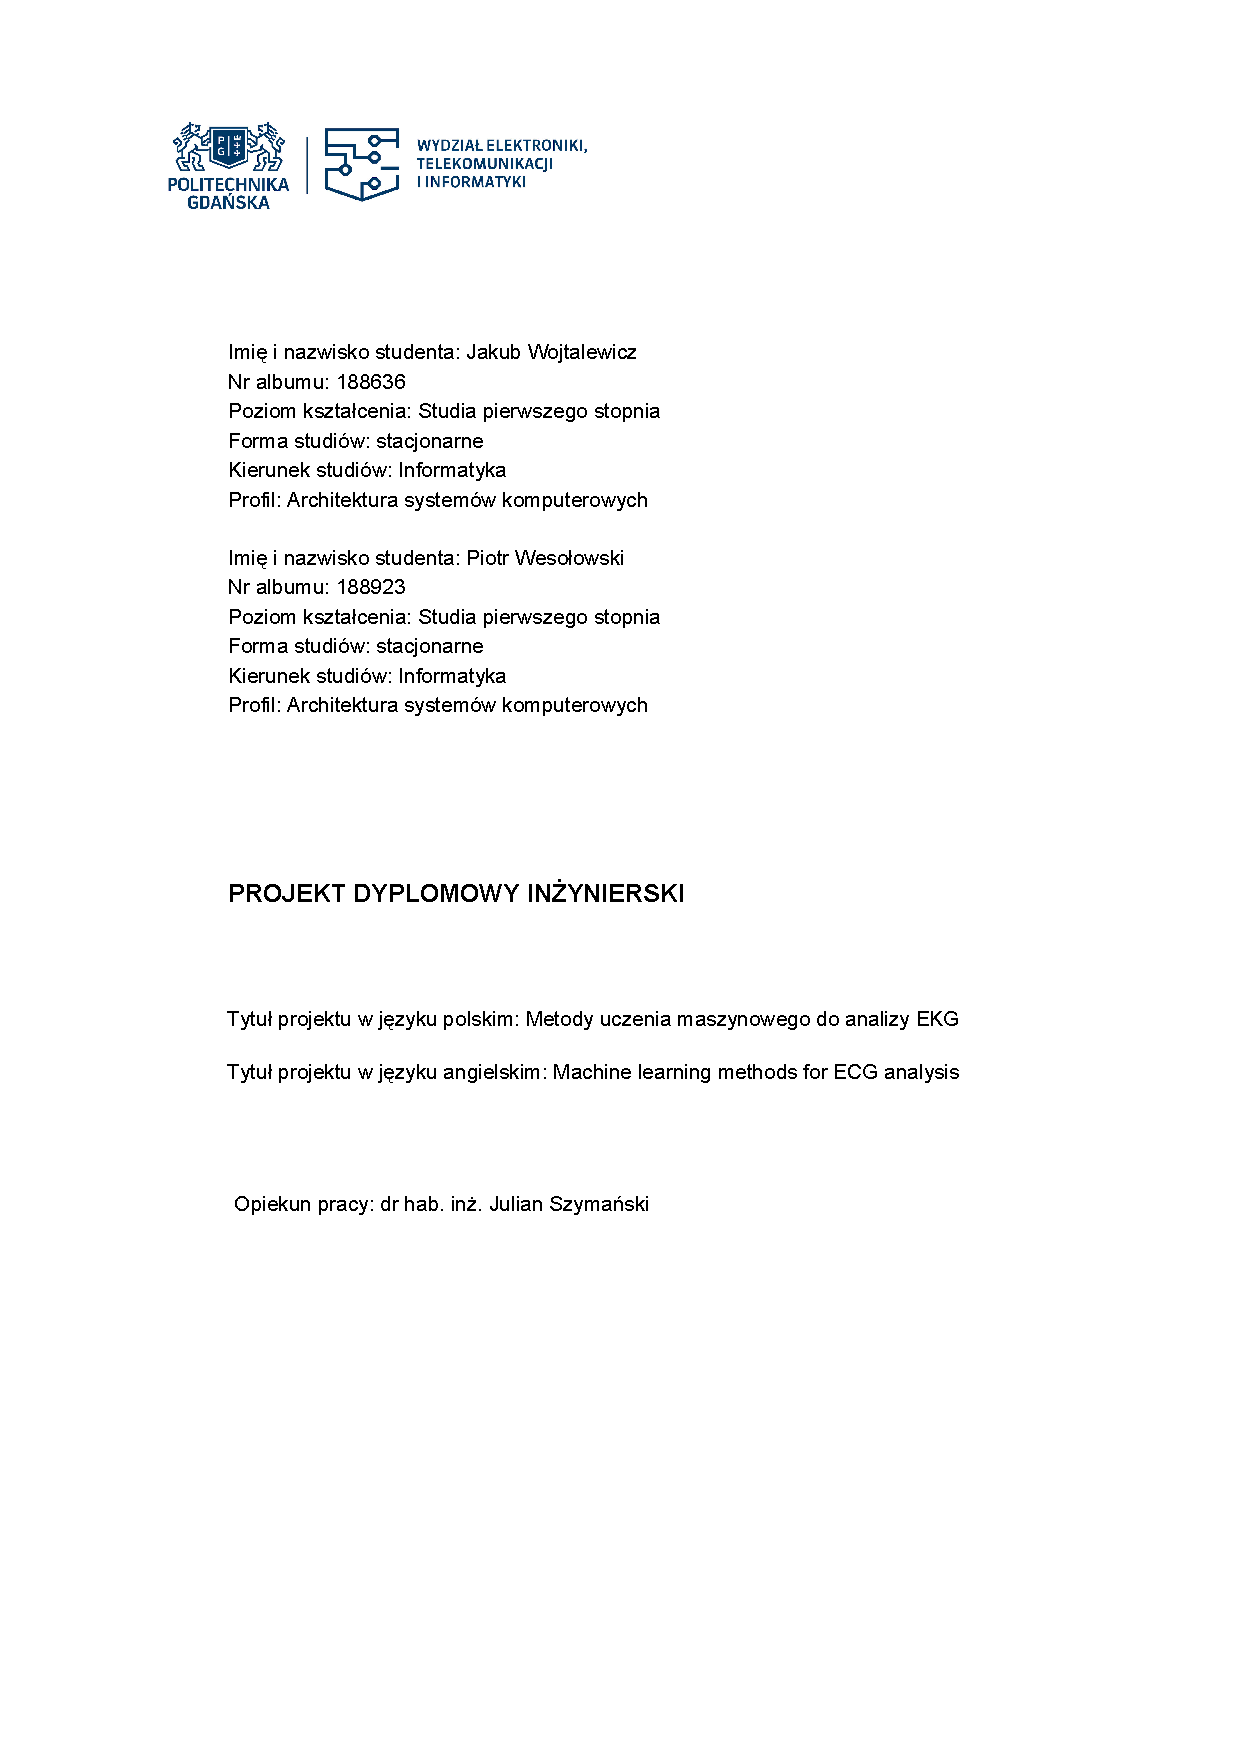
\includepdf{meta/StronaTytulowa.pdf}
% \chapter*{Streszczenie}
\indent Lorem Lorem ipsum dolor sit amet, consectetur adipiscing elit. Vivamus elementum arcu nec blandit aliquam. Integer eros dolor, molestie eget dictum quis, luctus sit amet sapien. Proin dignissim felis in ornare volutpat. Morbi vulputate rutrum efficitur. Ut vehicula vehicula metus, et iaculis tortor mattis vel. Nam blandit, arcu quis ultricies blandit, libero ante commodo augue, in accumsan dui leo at orci. Phasellus in augue et velit pulvinar malesuada ut et sem. Nulla vehicula nibh eu odio sollicitudin sagittis. Praesent condimentum semper neque, tincidunt luctus nisl scelerisque sed. Orci varius natoque penatibus et magnis dis parturient montes, nascetur ridiculus mus. 
\vspace{0.5cm}\newline
\textbf{S�owa kluczowe:} lorem ipsum, dolor sit amet, consectetur adipiscing\vspace{0.5cm}

\noindent \textbf{Dziedzina nauki i techniki, zgodnie z wymogami OECD:} nauki in�ynieryjne i techniczne, robotyka i automatyka

% \chapter*{Abstract \small{(author: Piotr Wesołowski)}}
\indent The engineering thesis presents a system for analyzing ECG signals using machine learning methods, focusing on heart rate variability (HRV) and the respiratory sinus arrhythmia (RSA) effect. The project is based on real-time data processing using the Polar H10 sensor and a dedicated application that enables the acquisition of ECG signals transmitted via Bluetooth. The system also supports the analysis of complete signal datasets loaded from files, allowing for comprehensive investigation of data dependencies.

The system implements various data analysis techniques, each requiring the prior identification of characteristic peaks in the ECG signal using a custom-developed algorithm. Based on the detected peaks, intervals between them were calculated, forming the foundation for further analysis. The primary analysis, performed in the time domain, allowed for the calculation of several key metrics based on these intervals. These intervals were also utilized in frequency and time-frequency analyses. Advanced mathematical transformations, such as the Fast Fourier Transform and wavelet analysis, were applied in these methods. The results of the analyses related to heart rate variability are presented as numerical values of key metrics and their time-varying characteristics on clear visual graphs.

The thesis compares the effectiveness of a traditional algorithm for R-peak detection with a machine learning-based algorithm. The applied neural networks achieved high accuracy in detecting characteristic peaks in the ECG signal and predicting various heart rate variability metrics based on them. An innovative approach was developed, enabling the prediction of HRV and RSA parameters directly from the entire ECG signal, representing a significant extension of the traditional RR-interval-based approach.

The thesis experimentally examined the impact of breathing patterns on RSA and analyzed the diurnal variability of heart activity by comparing differences between daytime and nighttime. A qualitative analysis of the developed neural network models was also conducted, highlighting their strengths, potential development directions, and possible applications in biomedical data analysis.

The system and methods presented in this thesis constitute a comprehensive platform for ECG analysis, with potential applications in scientific research and medical diagnostics.
\vspace{0.5cm}\newline
\textbf{Keywords:} Machine learning, EKG, HRV, RSA, Polar H10, end-to-end analysis \vspace{0.5cm}

\tableofcontents

\chapter{Wprowadzenie i cel pracy \small(autor: Piotr Weso�owski)}
Elektrokardiografia (EKG) to kluczowe narz�dzie diagnostyczne w analizie pracy serca, pozwalaj�ce na wykrywanie wielu nieprawid�owo�ci, b�d�cych jedn� z g��wnych przyczyn zgon�w na �wiecie \cite{Coronado-CVD-Global}. Poprawna analiza sygna�u EKG jest zadaniem niezwykle skomplikowanym i mimo licznych bada� w tym zakresie wci�� rozwijane s� nowe metody i podej�cia. Dzi�ki cyfrowemu zapisowi sygna�u serca mo�na stosowa� zaawansowane metody przetwarzania danych w analizie czasowej, cz�stotliwo�ciowej i nieliniowej. Rozwi�zanie to pozwala dostrzec r�nice, kt�re mog� pozosta� niewykryte podczas wizualnej analizy sygna�u przedstawionego na tradycyjnym wykresie na papierze milimetrowym.

Nowoczesne techniki analizy, takie jak eksploracja danych (data mining), pozwalaj� na uproszczenie monitorowania pracy serca w por�wnaniu z tradycyjnymi metodami. Z kolei metody uczenia maszynowego umo�liwiaj� wzrost efektywno�ci analizy sygna��w zaszumionych, kt�re stanowi� nieod��czny element d�u�szych rejestracji sygna�u. Podej�cie to eliminuje konieczno�� r�cznej korekcji, co jest czasoch�onne w klasycznych podej�ciach. Szczeg�lnym ich przyk�adem s� rozwi�zania end-to-end, oparte na analizie ca�ego sygna�u, kt�re pozwalaj� na tworzenie uniwersalnych modeli niezale�nie od aktualnie rozpatrywanego problemu. Tego rodzaju podej�cie wci�� nie jest zbyt szeroko opisane w literaturze naukowej, co stwarza przestrze� dla nowych bada� w tym zakresie.

W niniejszej pracy skupiono si� na wykorzystaniu zaawansowanych metod analitycznych, w tym sieci neuronowych, do analizy sygna�u EKG. G��wnym celem by�o opracowanie algorytmu umo�liwiaj�cego w czasie rzeczywistym wykrywanie kluczowych wzorc�w (np. za�amk�w R) oraz obliczanie wska�nik�w zmienno�ci rytmu serca (HRV) i analizy arytmii oddechowej (RSA). Opracowanie takiego rozwi�zania pozwala na kompleksow� i precyzyjn� analiz� sygna�u EKG zar�wno w badaniach naukowych, jak i w codziennej praktyce klinicznej.

\chapter{Podstawy teoretyczne}
Rozdzia� ten stanowi wprowadzenie teoretyczne do tematyki pracy, omawiaj�c
podstawowe poj�cia i kluczowe aspekty zwi�zane z analiz� sygna��w EKG, kt�re s�
istotne dla zrozumienia dalszych cz�ci opracowania. Przedstawiono tutaj og�lne za�o�enia dzia�ania elektrokardiografii, opis kluczowych sk�adowych sygna�u EKG oraz podstawowe parametry wykorzystywane w analizie zmienno�ci rytmu serca. Dokonano r�wnie� przegl�du metod uczenia maszynowego wykorzystywych w literaturze
naukowej do analizy sygna��w EKG.

\section{Elektrokardiografia \small{(autor: Jakub Wojtalewicz)}}

Elektrokardiografia, w skr�cie EKG, to badanie polegaj�ce na rejestracji
aktywno�ci elektrycznej serca. Zazwyczaj przyjmuje form� graficznego wykresu,
przedstawiaj�cego zmiany potencja��w elektrycznych serca w czasie
\cite{Lilly-Pathophysiology}. Rejestracja odbywa sie za pomoc� elektrod 
umieszczonych na ciele pacjenta w okre�lonych miejscach, takich jak klatka
piersiowa oraz ko�czyny, co pozwala na wychwycenie sygna��w bioelektrycznych
generowanych przez mi�sie� sercowy podczas jego pracy \cite{Romano-ECG}.

Badanie EKG jest istotnym narz�dziem diagnostycznym w medycynie przez swoj�
nieinwazyjno�� oraz pr�dko�� wykonania. Umo�liwia wykwalifikowanym lekarzom
ocen� stanu uk�adu sercowo-naczyniowego pacjenta oraz rozpoznanie wyst�puj�cych
nieprawid�owo�ci, kt�re mog� by� spowodowane wszelakimi schorzeniami
\cite{Malik-HRV}.

\section{Sk�adowe sygna�u EKG \small{(autor: Jakub Wojtalewicz)}}

% Sygna� EKG sk�ada si� z cyklicznie powtarzaj�cych si� fal i segment�w, kt�re odzwierciedlaj� r�ne fazy pracy serca. Cykl serca zaczyna sie za�amkiem P, odpowiadaj�cym za depolaryzacj� przedsionk�w serca, prowadz�cej do ich skurczu. Po nim nast�puje kompleks QRS, kt�ry jest odpowiedzialny za depolaryzacj� kom�r serca - kluczowego momentu skurczu mi�nia. Kompleks sk�ada sie z trzech fal: za�amka Q - pierwszego negatywnego w kompleksie - przedstawiaj�cego rozchodzenie si� impulsu elektrycznego w przegrodzie mi�dzykomorowej. Po nim nast�puje za�amek R - dodatni, zazwyczaj najbadziej widoczny komponent kompleksu - odzwierciedlaj�cy g�own� faz� depolaryzacji, kiedy wi�kszo�c masy mi�sniowej kom�r jest pobudzana do skurczu. Kompleks ko�czy kolejny za�amek negatywny S, reprezentuj�cy ko�cow� faz� depolaryzacji - na wykresie charakteryzuje go spadek poni�ej linii izoelektrycznej, bazowej wykresu. 

Sygna� EKG sk�ada si� z cyklicznie powtarzaj�cych si� fal i segment�w, kt�re
odzwierciedlaj� r�ne fazy pracy serca. Typowo segmenty te s� oznaczane kolejno
jako \textbf{P-QRS-T} Rys. \ref{fig/ekgGraph}. Cykl serca rozpoczyna si�
za�amkiem P, kt�ry odpowiada za depolaryzacj� przedsionk�w, prowadz�c� do ich
skurczu. Nast�pnie wyst�puje kompleks QRS, odpowiedzialny za depolaryzacj�
kom�r serca � kluczowy moment skurczu mi�nia sercowego. Kompleks ten sk�ada
si� z trzech fal:

\begin{itemize}
    \item \textbf{Za�amek Q} to pierwszy negatywny za�amek w kompleksie, kt�ry odzwierciedla pocz�tkow� faz� rozchodzenia si� impulsu elektrycznego przez przegrod� mi�dzykomorow�.
    \item \textbf{Za�amek R} jest dodatni i najcz�ciej najwi�kszy w ca�ym kompleksie. Reprezentuje g��wn� faz� depolaryzacji kom�r, kiedy wi�kszo�� masy mi�niowej zostaje pobudzona do skurczu.
    \item \textbf{Za�amek S} to kolejny negatywny za�amek, kt�ry zamyka kompleks QRS i reprezentuje ko�cow� faz� depolaryzacji kom�r, widoczn� jako spadek wykresu poni�ej linii izoelektrycznej.
\end{itemize}

Po kompleksie QRS pojawia si� za�amek T, kt�ry obrazuje repolaryzacj� kom�r,
czyli powr�t mi�nia sercowego do stanu spoczynkowego po skurczu. Za�amek T
jest zwykle dodatni i mniej wyra�ny ni� za�amek R, lecz jego kszta�t, czas
trwania oraz amplituda maj� istotne znaczenie diagnostyczne. Nieprawid�owo�ci w
za�amku T mog� wskazywa� na problemy takie jak niedokrwienie mi�nia sercowego,
zaburzenia elektrolitowe lub inne patologie repolaryzacyjne.

Ca�y cykl serca przedstawiony w sygnale EKG odzwierciedla skoordynowane zmiany
elektryczne zachodz�ce w sercu, dostarczaj�c szczeg�owych informacji o jego
funkcjonowaniu. Ka�dy komponent ma kluczowe znaczenie diagnostyczne,
umo�liwiaj�c ocen� stanu uk�adu sercowo-naczyniowego oraz identyfikacj�
r�norodnych zaburze� i patologii sercowych \cite{Romano-ECG}.

\begin{figure}[ht]
    \centering
    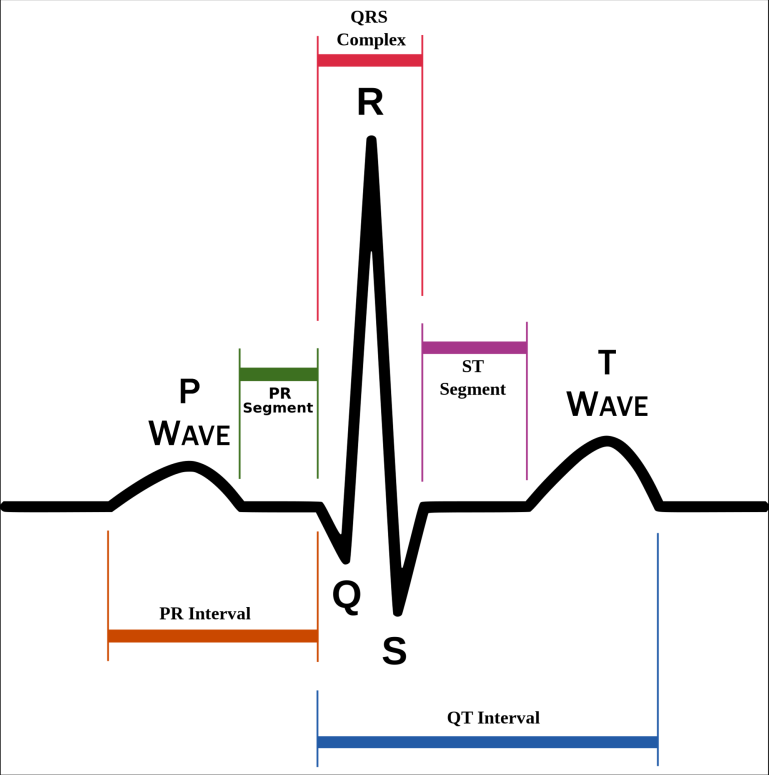
\includegraphics[scale=0.25]{Rysunki/Normal-ECG-signal-with-his-different-features.png}
    \caption{Normalny sygna� EKG z jego cechami.}
    \caption*{�r�d�o:  \url{https://www.researchgate.net/figure/Normal-ECG-signal-with-his-different-features_fig1_299575422} [Data uzyskania dost�pu 02.11.2024]}
    \label{fig/ekgGraph}
\end{figure}

\section{Charakterystyki sygna�u EKG \small{(autor: Piotr Weso�owski)}}\label{MiaryHRV}

Podczas analizy sygna�u EKG wyr�ni� mo�na wiele charakterystyk, kt�re
dostarczaj� szczeg�owych informacji o pracy serca i kondycji uk�adu
sercowo-naczyniowego badanej osoby.

\subsection{Odst�py RR i puls}

Jednym z kluczowych parametr�w opisuj�cych sygna� EKG jest czas pomi�dzy kolejnymi szczytami za�amk�w R, wyra�any w milisekundach (ms). Parametr ten nazywany jest \textit{odst�pem RR} (ang. \textit{RR interval}). W literaturze wyst�puje r�wnie� okre�lenie \textit{odst�p NN} (ang. \textit{NN interval}), kt�re odnosi si� do odst�p�w pomi�dzy kolejnymi za�amkami R, ale z uwzgl�dnieniem wy��cznie rytmu prawid�owego, pozbawionego artefakt�w i zak��ce� (ang. \textit{normal-to-normal}). Chocia� w praktyce oba terminy bywaj� u�ywane zamiennie, w analizach dotycz�cych pracy serca kluczowe jest, aby uwzgl�dnia� jedynie prawid�owy rytm, wolny od znacz�cych zak��ce� i artefakt�w. Jego analiza pozwala bezpo�rednio okre�li� inn� istotn� metryk�, jak� jest puls, czyli \textit{HR} (ang. \textit{heart rate}), kt�ry oznacza liczb� uderze� serca na minut�. Ka�demu skurczowi serca towarzyszy charakterystyczny wzrost potencja�u elektrycznego, rejestrowany jako szczyt $R$ na wykresie EKG \cite{Zhan-RWave}.

Chwilowe t�tno w chwili \( t_{R_n} \), czyli w momencie wyst�pienia \( n \)-tego szczytu \( R \), mo�na wyrazi� za pomoc� wzoru:

\begin{equation}  
    HR_n = \frac{60}{t_{R_n} - t_{R_{n-1}}}
\end{equation}

gdzie:

\begin{itemize}
    \item \( t_{R_n} \) to czas wyst�pienia \( n \)-tego szczytu \( R \),
    \item \( t_{R_{n-1}} \) to czas wyst�pienia poprzedniego szczytu \( R \),
    \item wynik \( HR_n \) wyra�ony jest w uderzeniach na minut� (bpm, \textit{beats per minute}).\\
\end{itemize}



Je�li jednak chcieliby�my przybli�y� warto�� t�tna w dowolnym punkcie pomi�dzy szczytami, nale�a�oby t� warto�� odpowiednio ekstrapolowa�.

Wielko�� r�nic pomi�dzy kolejnymi odst�pami RR (tzw. \textit{RR variability}) jest kolejnym kluczowym wska�nikiem pracy serca. Analiza tych r�nic, wykorzystuj�c miary czasowe i cz�stotliwo�ciowe, jest podstaw� do okre�lenia zmienno�ci rytmu serca, szeroko opisywanej w dalszej cz�ci tej pracy.


\subsection{Analiza w domenie czasowej}

Metody analizy czasowej opieraj� si� na bezpo�rednim pomiarze odst�p�w RR w sygnale EKG, kt�re reprezentuj� czas mi�dzy kolejnymi skurczami serca. Poni�ej przedstawiono podstawowe miary analizy czasowej:

\subsubsection{SDNN} \label{SDNN}
{SDNN} (ang. \textit{Standard Deviation of NN intervals}), czyli odchylenie standardowe wszystkich odst�p�w RR w badanym okresie, jest jedn� z podstawowych miar zmienno�ci rytmu serca. Warto�� SDNN odzwierciedla ca�kowit� zmienno�� sygna�u rytmu serca, poniewa� wariancja sygna�u, b�d�ca kwadratem odchylenia standardowego, jest r�wna sumie mocy w ca�ym zakresie cz�stotliwo�ci \cite{Saul1988}. SDNN jest prost� miar� do obliczenia, jednak nie jest dobrze zdefiniowan� zmienn� statystyczn�, poniewa� jej warto�� zale�y od d�ugo�ci badania. Wielko�� SDNN wzrasta wraz z czasem trwania rejestracji, dlatego por�wnywanie wynik�w mi�dzy badaniami o r�nej d�ugo�ci wymaga wcze�niejszej normalizacji do okre�lonych okres�w, np. do nominalnych zapis�w 24-godzinnych lub kr�tkoterminowych trwaj�cych 5 minut.

\begin{equation}
  \text{SDNN} = \sqrt{\frac{1}{N-1} \sum_{i=1}^{N} \left( RR_i - \overline{RR} \right)^2}
\end{equation}

gdzie:

\begin{itemize}
  \item \(RR_i\) to kolejne odst�py RR (czas mi�dzy kolejnymi uderzeniami serca),
  \item \(\overline{RR}\) to �rednia warto�� odst�p�w RR,
  \item \(N\) to liczba wszystkich pomiar�w odst�p�w RR, czyli liczba zmierzonych interwa��w RR w analizowanym okresie czasu.\\
\end{itemize}

\subsubsection{RMSSD}
{RMSSD} (ang. \textit{Root Mean Square of Successive Differences}), czyli pierwiastek ze �redniej kwadratowej r�nic pomi�dzy kolejnymi odst�pami RR, jest miar� szczeg�lnie u�yteczn� w ocenie kr�tkoterminowych waha� rytmu serca i  dosy� precyzyjnie wskazuje na aktywno�� przywsp�czuln� uk�adu nerwowego \cite{Schneider-PTSD}. Dzi�ki temu jest mniej podatne na wp�yw d�ugoterminowych fluktuacji oraz artefakt�w, co czyni je jedn� z najcz�ciej stosowanych miar kr�tkoterminowej zmienno�ci rytmu serca.
\begin{equation}
  \text{RMSSD} = \sqrt{\frac{1}{N-1} \sum_{i=1}^{N-1} \left( RR_{i+1} - RR_i \right)^2}
\end{equation}


gdzie:

\begin{itemize}
  \item \(RR_i\) i \(RR_{i+1}\) to kolejne odst�py RR (czas mi�dzy kolejnymi uderzeniami serca),
  \item \(N\) to liczba pomiar�w odst�p�w RR u�ywanych do obliczenia RMSSD, czyli liczba interwa��w RR uwzgl�dniona w analizowanym okresie czasu (zwykle w analizie 5-minutowej lub d�u�szej).
\end{itemize}

\subsubsection{NN50 i pNN50}
{NN50} (ang. \textit{Number of NN intervals differing by more than 50 ms}) to liczba odst�p�w RR, dla kt�rych r�nica pomi�dzy kolejnymi warto�ciami przekracza 50 ms. Jest to miara czasowa, kt�ra pozwala na ocen� kr�tkoterminowych waha� rytmu serca:
\begin{equation}
  \text{NN50} = \sum_{i=1}^{N-1} \mathbf{1} \left( |RR_{i+1} - RR_i| > 50 \, \text{ms} \right)
\end{equation}

gdzie:

\begin{itemize}
  \item \(RR_i\) i \(RR_{i+1}\) to kolejne odst�py RR (czas mi�dzy kolejnymi uderzeniami serca),
  \item \(\mathbf{1} \left( \cdot \right)\) to funkcja wska�nikowa, kt�ra przyjmuje warto�� 1, je�li warunek w nawiasie jest spe�niony (czyli r�nica mi�dzy kolejnymi odst�pami RR jest wi�ksza ni� 50 ms), a 0 w przeciwnym przypadku,
  \item \(N\) to liczba pomiar�w odst�p�w RR u�ywanych do obliczenia NN50, czyli liczba interwa��w RR w analizowanym okresie czasu.\\
\end{itemize}

Nast�pnie, {PNN50} (ang. \textit{Proportion of NN50 intervals to the total number of NN intervals}) to procent tych r�nic w stosunku do ca�kowitej liczby odst�p�w RR:

\begin{equation}
  \text{pNN50} = \frac{\text{NN50}}{N-1} \times 100
\end{equation}

gdzie:

\begin{itemize}
  \item \(N-1\) to liczba par odst�p�w RR (czyli r�nic mi�dzy kolejnymi odst�pami),
  \item \(\text{NN50}\) to liczba par odst�p�w RR, kt�rych r�nica jest wi�ksza ni� 50 ms.\\
\end{itemize}

pNN50 jest silnie skorelowana z RMSSD \cite{Malik-HRV}, jednak�e to ta druga miara jest cz�ciej u�ywana w nomenklaturze do oceny kr�tkoterminowych zmienno�ci
\subsubsection{SDANN}
{SDANN} (ang. \textit{Standard Deviation of the Averages of NN intervals}), czyli odchylenie standardowe �rednich odst�p�w NN obliczonych dla kr�tkich segment�w czasowych, takich jak 5-minutowe odcinki, jest miar� d�ugoterminowej zmienno�ci rytmu serca. Proces obliczania SDANN polega na podzieleniu ca�ego okresu rejestracji, np. 24-godzinnego, na kr�tsze segmenty (np. 5-minutowe), a nast�pnie obliczeniu �rednich odst�p�w NN dla ka�dego z nich. Odchylenie standardowe tych �rednich warto�ci jest finaln� warto�ci� SDANN, co czyni t� miar� szczeg�lnie przydatn� w analizie d�ugoterminowych zmian rytmu serca, takich jak r�nice mi�dzy dniem a noc�.
\begin{equation}
  \text{SDANN} = \sqrt{\frac{1}{M-1} \sum_{j=1}^{M} \left( \overline{NN}_j - \overline{\overline{NN}} \right)^2}
\end{equation}

gdzie:

\begin{itemize}
  \item \(M\) to liczba segment�w czasowych, w kt�rych analizowane s� odst�py NN. Na przyk�ad, je�li dane s� podzielone na segmenty 5-minutowe, to \(M\) to liczba tych segment�w,
  \item \(\overline{NN}_j\) to �rednia warto�� odst�p�w NN w \(j\)-tym segmencie czasowym,
  \item \(\overline{\overline{NN}}\) to �rednia wszystkich �rednich, czyli �rednia z \(\overline{NN}_j\) dla wszystkich segment�w.
\end{itemize}

\subsubsection{SDNN Index}
SDNN Index jest �redni� warto�ci� odchylenia standardowego odst�p�w NN dla wszystkich 5-minutowych segment�w ca�ego okresu rejestracji. R�ni si� on od SDANN tym, �e odnosi si� do kr�tkoterminowej zmienno�ci rytmu serca w obr�bie poszczeg�lnych segment�w. Ta miara jest u�ywana do oceny bardziej szczeg�owych zmian w rytmie serca w kr�tszych przedzia�ach czasowych.
\begin{equation}
  \text{SDNN Index} = \frac{1}{M} \sum_{j=1}^{M} \sqrt{\frac{1}{N_j-1} \sum_{i=1}^{N_j} \left( RR_{i,j} - \overline{RR}_j \right)^2}
\end{equation}

gdzie:

\begin{itemize}
  \item \(M\) to liczba segment�w czasowych, w kt�rych dane s� podzielone,
  \item \(N_j\) to liczba odst�p�w RR w \(j\)-tym segmencie, czyli liczba interwa��w RR, kt�re zosta�y zmierzone w \(j\)-tym segmencie,
  \item \(\overline{RR}_j\) to �rednia warto�� odst�p�w RR w \(j\)-tym segmencie.
\end{itemize}


\subsection{Analiza w domenie cz�stotliwo�ciowej}

Analiza cz�stotliwo�ciowa pozwala przekszta�ci� sygna� z dziedziny czasu na dziedzin� cz�stotliwo�ci, co umo�liwia ocen� mocy sygna�u w r�nych pasmach. Kluczowym narz�dziem tej analizy jest transformacja Fouriera, kt�ra identyfikuje obecne w sygnale cz�stotliwo�ci oraz przypisan� im moc. Dok�adna dekompozycja sygna�u jest operacj� bardzo z�o�on� obliczeniowo i czasowo, dlatego w praktyce stosuje si� {FFT} (ang. \textit{Fast Fourier Transform}), czyli szybk� transformacj� Fouriera, kt�ra umo�liwia efektywn� analiz� mocy widmowej ({PSD} (ang. \textit{Power Spectral Density})), nale�y jednak pami�ta� �e uzyskany w ten spos�b wynik to jedynie oszacowanie rzeczywistej mocy. Analiza ta zak�ada stacjonarno�� sygna�u w badanym przedziale czasowym, co mo�e by� problematyczne w przypadku sygna��w biologicznych, takich jak rytm serca czy oddech. Z tego powodu FFT najlepiej sprawdza si� w badaniach, gdzie sygna�y s� wzgl�dnie stabilne, np. podczas spokojnego oddychania. W sytuacjach, gdy wyst�puj� zmiany w rytmie oddechowym i t�tnie (np. w wyniku dzia�ania stresora), analiza FFT mo�e wykaza� umiarkowan� moc w szerokim zakresie cz�stotliwo�ci, co utrudnia identyfikacj� dominuj�cych pasm. Dlatego analizy cz�stotliwo�ciowe s� najcz�ciej wykonywane na sygna�ach trwaj�cych oko�o 5 minut \cite{Malik-HRV}.
\begin{equation}  
  \text{PSD}(f) = \left| \int_{-\infty}^{\infty} x(t) e^{-j 2 \pi f t} dt \right|^2
\end{equation}

gdzie:

\begin{itemize}
  \item \(\text{PSD}(f)\) to g�sto�� widmowa mocy sygna�u \(x(t)\) w funkcji cz�stotliwo�ci \(f\),
  \item \(x(t)\) to sygna� w dziedzinie czasu,
  \item \(e^{-j 2 \pi f t}\) to funkcja wyk�adnicza, kt�ra reprezentuje transformacj� Fouriera,
  \item \(\int_{-\infty}^{\infty} x(t) e^{-j 2 \pi f t} dt\) to transformata Fouriera sygna�u \(x(t)\) w dziedzinie cz�stotliwo�ci.\\
\end{itemize}

Moc sygna�u w danym pa�mie cz�stotliwo�ci oblicza si� jako:

\begin{equation}
  \text{Moc w pa�mie} = \int_{f_{\text{min}}}^{f_{\text{max}}} \text{PSD}(f) df
\end{equation}

gdzie:

\begin{itemize}
  \item \(f_{\text{min}}\) i \(f_{\text{max}}\) to granice cz�stotliwo�ci, kt�re definiuj� pasmo, w kt�rym obliczana jest moc sygna�u,
  \item \(\text{PSD}(f)\) to warto�� g�sto�ci widmowej mocy w cz�stotliwo�ci \(f\),
  \item ca�kowanie po \(f\) w granicach \(f_{\text{min}}\) i \(f_{\text{max}}\) pozwala na obliczenie ca�kowitej mocy w danym pa�mie.\\
\end{itemize}

Powszechnie analizowane pasma to \cite{Malik-HRV}:

\begin{itemize}
    \item \textbf{ULF} (ang. \textit{Ultra Low Frequency}) (<0.003 Hz): Odzwierciedla mechanizmy hormonalne oraz inne wolnozmienne procesy fizjologiczne.
    \item \textbf{VLF} (ang. \textit{Very Low Frequency}) (0.003�0.04 Hz): Zwi�zane z procesami termoregulacji i innymi mechanizmami o niskiej cz�stotliwo�ci.
    \item \textbf{LF} (ang. \textit{Low Frequency}) (0.04�0.15 Hz): Odzwierciedla aktywno�� wsp�czuln� i przywsp�czuln� oraz barorefleksj� kt�ra odpowiada za utrzymanie ci�nienia krwi na sta�ym poziomie.
    \item \textbf{HF} (ang. \textit{High Frequency}) (0.15�0.4 Hz): Powi�zane z rytmem oddechowym i aktywno�ci� przywsp�czuln�, szczeg�lnie widoczne u zdrowych os�b.
    \item \textbf{UHF} (ang. \textit{Ultra High Frequency}) (> 0.4 Hz):  Rzadko analizowane, mo�e obejmowa� szybkie zmiany fizjologiczne, ale tak�e zak��cenia i artefakty zwi�zane z pomiarem.\\
\end{itemize}

W analizie cz�stotliwo�ciowej stosuje si� r�wnie� wska�niki znormalizowane, takie jak \textit{LF norm} i \textit{HF norm}, kt�re pozwalaj� oceni� moc w poszczeg�lnych pasmach w odniesieniu do ca�kowitej mocy sygna�u:

\begin{equation}
  \text{LF}_{\text{norm}} = \frac{\text{LF}}{\text{LF} + \text{HF}} \cdot 100, \quad
  \text{HF}_{\text{norm}} = \frac{\text{HF}}{\text{LF} + \text{HF}} \cdot 100\\
\end{equation}


Dodatkowo, wska�nik \textit{LF/HF} jest powszechnie stosowany jako miara r�wnowagi mi�dzy uk�adem wsp�czulnym a przywsp�czulnym, cho� jego interpretacja mo�e by� niejednoznaczna:

\begin{equation}
  \text{LF/HF} = \frac{\text{LF}}{\text{HF}}
\end{equation}

gdzie:
\begin{itemize}
    \item LF � moc w niskich cz�stotliwo�ciach (Low Frequency),
    \item HF � moc w wysokich cz�stotliwo�ciach (High Frequency),
    \item $\text{LF} + \text{HF}$ � ca�kowita moc sygna�u w analizowanych pasmach.
\end{itemize}

\subsection{Analiza w dziedzinie czasowo-cz�stotliwo�ciowej}

Analiza czasowo-cz�stotliwo�ciowa pozwala na jednoczesne okre�lenie mocy sygna�u w wybranych pasmach cz�stotliwo�ci i ich zmian w czasie. W przeciwie�stwie do klasycznej analizy cz�stotliwo�ciowej, kt�ra zak�ada stacjonarno�� sygna�u, analiza czasowo-cz�stotliwo�ciowa uwzgl�dnia zmienno�� sygna�u w czasie \cite{Boashash1992}.

\begin{equation}
  W_x(a, b) = \int_{-\infty}^{\infty} x(t) \psi^* \left( \frac{t-b}{a} \right) dt
\end{equation}

gdzie:

\begin{itemize}
  \item \( x(t) \) to sygna� w dziedzinie czasu, kt�ry jest analizowany,
  \item \( \psi(t) \) to funkcja falki (ang. wavelet), kt�ra jest podstawow� funkcj� w analizie falkowej,
  \item \( a \) to skala, kt�ra kontroluje rozci�gni�cie lub kompresj� funkcji falki w czasie,
  \item \( b \) to przesuni�cie czasowe, kt�re okre�la, w kt�rym punkcie czasowym funkcja falki jest analizowana,
  \item \( \psi^* \) to sprz�enie zespolone funkcji falki.\\
\end{itemize}

W sytuacjach, w kt�rych rytm serca i oddechu zmieniaj� si� w czasie, przydatnym narz�dziem jest analiza falkowa, np. z u�yciem falki Morleta. Pozwala ona analizowa� sygna� jednocze�nie w domenie czasowej i cz�stotliwo�ciowej, co umo�liwia �ledzenie, jak zmienia si� moc w okre�lonych cz�stotliwo�ciach w czasie. W tym celu wykorzystuje zestaw funkcji zwanych falami, kt�re s� odpowiednio przesuwane oraz skalowane (�ciskane lub rozci�gane), aby dopasowa� je do analizy kr�tkotrwa�ych zjawisk o wysokiej cz�stotliwo�ci lub d�ugotrwa�ych zjawisk o niskiej cz�stotliwo�ci. Dzi�ki temu mo�na oceni� aktywno�� uk�ad�w regulacyjnych (np. przywsp�czulnego) w okre�lonych przedzia�ach czasowych, np oddzielnie dla relaksu, stresu, aktywno�ci fizycznej czy �wicze� oddechowych \cite{Boashash1992}.


Wyniki analizy falkowej s� cz�sto przedstawiane na skalogramie czyli  graficznej reprezentacji mocy sygna�u w zale�no�ci od czasu i cz�stotliwo�ci. Przedstawia on zmiany mocy w formie kolorowego wykresu, gdzie o� X reprezentuje czas, o� Y � cz�stotliwo��, a kolory � moc sygna�u.

\begin{equation}
  S(a, b) = |W_x(a, b)|^2
\end{equation}

gdzie:

\begin{itemize}
  \item \( S(a, b) \) to skalogram, kt�ry przedstawia intensywno�� sygna�u \( x(t) \) w funkcji skali \( a \) i przesuni�cia \( b \),
  \item \( W_x(a, b) \) to wsp�czynnik transformacji falkowej dla danej skali \( a \) i przesuni�cia \( b \),
  \item \( |W_x(a, b)|^2 \) to kwadrat modu�u wsp�czynnika transformacji, kt�ry reprezentuje intensywno�� sygna�u na okre�lonej skali i w okre�lonym czasie.
\end{itemize}

\section{HRV \small{(autor: Piotr Weso�owski)}}
\subsection{Wprowadzenie}
{HRV} (ang. \textit{Heart Rate Variability}) oznacza zmienno�� rytmu pracy serca, czyli r�nice w czasie pomi�dzy kolejnymi szczytami R w sygnale EKG. Za jej pomoc� mo�na okre�li�, jak serce reaguje na r�ne warunki, takie jak stres, aktywno�� fizyczna czy zmiany w oddychaniu. Warto�� t� mo�na analizowa� za pomoc� metod czasowych, cz�stotliwo�ciowych, czasowo-cz�stotliwo�ciowych, a tak�e geometrycznych (te ostatnie nie s� rozwijane w niniejszej pracy). Dob�r konkretnej metody analizy zale�y od charakterystyki badania, takiej jak czas jego trwania, stacjonarno�� rytmu serca czy wp�yw stresor�w. Znaczenie i interpretacja uzyskanych wynik�w s� istotne dla oceny pracy serca i cz�sto bardziej z�o�one, ni� si� powszechnie uwa�a, co mo�e prowadzi� do b��dnych wniosk�w.

\subsection{Podzia� miar HRV}
Do oceny HRV mo�na wykorzysta� miary podzielone na dwie grupy w zale�no�ci od rodzaju danych s�u��cych do ich oblicze� \cite{Malik-HRV}:

\subsection*{Miary oparte na bezpo�rednich d�ugo�ciach odst�p�w RR}
\begin{itemize}
    \item \textbf{S�u��ce do og�lnej oceny zmienno�ci rytmu serca:}
    \begin{itemize}
        \item SDNN,
        \item r�nica mi�dzy najd�u�szym a najkr�tszym odst�pem RR.
    \end{itemize}
    \item \textbf{S�u��ce do oceny d�ugoterminowych zmienno�ci HRV, wynikaj�cych m.in. z r�nic podczas cyklu dobowego czy aktywno�ci fizycznej:}
    \begin{itemize}
        \item SDANN.
    \end{itemize}
\end{itemize}

\subsection*{Miary oparte na r�nicach mi�dzy kolejnymi odst�pami RR}
\begin{itemize}
    \item \textbf{S�u��ce do oceny kr�tkoterminowych zmienno�ci HRV, cz�sto u�ywane do oceny aktywno�ci przywsp�czulnej:}
    \begin{itemize}
        \item RMSSD,
        \item SDNN Index,
        \item pNN50.
    \end{itemize}
\end{itemize}


\subsection{Analiza cz�stotliwo�ciowa HRV}
Do analizy cz�stotliwo�ciowej HRV wykorzystuje si� nast�puj�ce wska�niki \cite{Malik-HRV}:
\begin{itemize}
    \item \textbf{Moc w pa�mie HF (wysokiej cz�stotliwo�ci):} Silnie skorelowana z aktywno�ci� uk�adu przywsp�czulnego. Zazwyczaj wzrasta w wyniku kontrolowanego oddychania oraz pod wp�ywem takich czynnik�w jak stymulacja narz�du r�wnowagi czy stymulacja twarzy zimnem. HF mo�e by� r�wnie� modyfikowane przez rytm oddechowy, co wymaga jego kontroli w trakcie badania.
    \item \textbf{Moc w pa�mie LF (niskiej cz�stotliwo�ci):} Cz�sto uznawana za marker aktywno�ci wsp�czulnej, cho� wi�kszo�� badaczy uwa�a, �e odzwierciedla wp�yw obu uk�ad�w autonomicznych. Jej warto�� wzrasta m.in. w wyniku stresu, wysi�ku fizycznego, a tak�e przy zmianie pozycji na stoj�c� lub bardziej pionow�. Interpretacja LF wymaga ostro�no�ci, poniewa� mo�e by� podatna na zak��cenia niefizjologiczne, takie jak artefakty ruchowe.
\end{itemize}

\subsection{Normalizacja i wska�niki dodatkowe}
Moc w okre�lonym pa�mie zale�y od d�ugo�ci rejestrowanego sygna�u. Dlatego, opr�cz zalecanej d�ugo�ci badania wynosz�cej 5 minut, stosuje si� wska�niki w jednostkach znormalizowanych [nu.].
Wska�niki te s� bardziej wiarygodne przy umiarkowanych lub wysokich warto�ciach ca�kowitej mocy HRV ({TP}, ang. Total Power), kt�ra odzwierciedla og�ln� zmienno�� rytmu serca. W stanach obni�onej zmienno�ci rytmu serca, takich jak silny stres, choroby czy zaawansowany wiek, interpretacja tych wska�nik�w mo�e prowadzi� do b��dnych wniosk�w. Stosunek LF/HF jest cz�sto wykorzystywany jako wska�nik r�wnowagi mi�dzy aktywno�ci� uk�adu wsp�czulnego i przywsp�czulnego, jednak jego wysokie warto�ci mog� wynika� zar�wno ze zwi�kszonej aktywno�ci wsp�czulnej, jak i os�abienia aktywno�ci przywsp�czulnej \cite{Malik-HRV}.

\subsection{Analiza d�ugoterminowa}

W badaniach trwaj�cych 24 godziny, kt�re umo�liwiaj� ocen� HRV w ci�gu ca�ej doby, wiele zmiennych z dziedziny czasu i cz�stotliwo�ci jest ze sob� skorelowanych. Je�li nie zamierzamy stosowa� dodatkowych miar, takich jak nachylenie log-log skalogramu w analizie spektralnej, wyniki pomiar�w z dziedziny czasu s� niemal to�same z wynikami z analizy cz�stotliwo�ciowej. Jednocze�nie s� one �atwiejsze do uzyskania i interpretacji. 

Nale�y jednak pami�ta�, �e metody czasowe lepiej sprawdzaj� si� w analizie d�ugoterminowych rejestracji ze wzgl�du na brak stabilno�ci sygna�u w ca�ym zakresie, podczas gdy metody cz�stotliwo�ciowe s� bardziej odpowiednie do oceny kr�tkoterminowych zmienno�ci rytmu serca \cite{Malik-HRV}.

\subsection{Artefakty i jako�� sygna�u}

HRV jest bardzo wra�liwe na artefakty w zapisie EKG (np. b��dy detekcji R-R lub ruch pacjenta). Dlatego kluczowym etapem analizy jest usuni�cie artefakt�w oraz weryfikacja poprawno�ci detekcji szczyt�w R w sygnale EKG, co pozwala unikn�� zniekszta�cenia wynik�w.

\subsection{Zale�no�� HRV od czynnik�w demograficznych i zdrowotnych}

Warto podkre�li�, �e HRV silnie zale�y od takich czynnik�w jak wiek, p�e� czy stan zdrowia. Na przyk�ad og�lna zmienno�� HRV (\textit{SDNN}) spada z wiekiem, a r�nice mi�dzy p�ciami mog� wynika� z odmiennej aktywno�ci uk�adu autonomicznego. Interpretacja wynik�w powinna zawsze uwzgl�dnia� te konteksty \cite{Malik-HRV}.

\subsection{Interpretacja wynik�w}
W celu rzetelnej oceny zmienno�ci rytmu serca w dziedzinie czasu nale�y interpretowa� jednocze�nie wyniki opisuj�ce og�ln� zmienno�� (np. SDNN) oraz sk�adniki kr�tkoterminowe i d�ugoterminowe (odpowiednio RMSSD i SDANN). Analogicznie, w analizie cz�stotliwo�ciowej oraz czasowo-cz�stotliwo�ciowej kluczowe znaczenie maj� miary mocy w r�nych pasmach widmowych (np. HF i LF). Nic nie stoi na przeszkodzie, aby analizowa� poszczeg�lne sk�adniki z perspektywy r�nych metod.

Wy�sze warto�ci zar�wno metryk czasowych, jak i cz�stotliwo�ciowych (np. moc w analizowanych pasmach) wskazuj� na wy�sze og�lne HRV, co zazwyczaj jest uwa�ane za korzystne dla zdrowia. Nale�y jednak pami�ta�, �e kluczowe dla oceny zdrowotnej zmienno�ci rytmu serca jest proporcja sk�adnik�w odpowiadaj�cych r�nym mechanizmom regulacyjnym.

O ile wysokie warto�ci HRV s� og�lnie pozytywne, to ich zdrowotne znaczenie wzrasta, gdy wynikaj� z wysokiej mocy w pa�mie HF, co wskazuje na prawid�owe i intensywne dzia�anie uk�adu przywsp�czulnego. Taka sytuacja zwykle jest zwi�zana z regularnym oddechem lub efektywnymi reakcjami relaksacyjnymi.

Z kolei w badaniach, w kt�rych og�lna zmienno�� rytmu serca (np. SDNN lub ca�kowita moc) jest wysoka, ale dominuje wp�yw pasma LF, mo�e to oznacza�, �e rytm serca jest zmienny g��wnie z powodu zwi�kszonej aktywno�ci wsp�czulnej. Taka sytuacja mo�e by� zwi�zana ze stresem, przeci��eniem organizmu lub nawet stanami patologicznymi, takimi jak arytmie \cite{Malik-HRV}.
\subsection{Podsumowanie}

Nale�y pami�ta�, �e HRV mierzy zmienno�� rytmu pracy serca, a nie jego �redni poziom. Zgodnie z obecn� wiedz� medyczn�, w�a�ciwa ocena HRV jest trudna, lecz mo�e znacznie przyczyni� si� do lepszego zrozumienia mechanizm�w reguluj�cych rytm serca oraz ich powi�za� z procesami fizjologicznymi i stanami chorobowymi. 

Badanie HRV, zw�aszcza jego d�ugookresowych fluktuacji, stanowi cenny wska�nik stanu zdrowia w wielu zaburzeniach. Na przyk�ad po zawale mi�nia sercowego pozwala z wysok� dok�adno�ci� oszacowa� przewidywany czas prze�ycia, niezale�nie od innych parametr�w \cite{Kleiger-HRV-Mortality}.


\section{RSA \small{(autor: Piotr Weso�owski)}}



{RSA} (ang. \textit{Respiratory Sinus Arrhythmia}) to zjawisko polegaj�ce na cyklicznych i skorelowanych z cyklami oddechowymi zmianach w cz�stotliwo�ci rytmu serca. Wynika ono z interakcji mi�dzy uk�adem oddechowym, kr��eniowym i nerwowym \cite{Hayano1996}.

\subsection{Mechanizm RSA}

Podczas wdechu przepona kurczy si� i przesuwa w d�, co zwi�ksza obj�to�� klatki piersiowej i powoduje spadek ci�nienia wewn�trzklatkowego. Obni�one ci�nienie u�atwia powr�t �ylny do serca oraz obj�to�� wyrzutow�, a jednocze�nie powoduje zmniejszenie aktywno�ci nerwu b��dnego (przywsp�czulnego), co prowadzi do wzrostu cz�sto�ci rytmu serca.

Podczas wydechu przepona rozlu�nia si� i wraca w g�r�, zmniejszaj�c obj�to�� klatki piersiowej. To powoduje wzrost ci�nienia wewn�trzklatkowego, co zmniejsza powr�t �ylny i obj�to�� wyrzutow� serca. W tym samym czasie wzrasta aktywno�� nerwu b��dnego, co skutkuje spowolnieniem rytmu serca.

Te zmiany s� dodatkowo modulowane przez mechanizm barorefleksji, kt�ry odpowiada za utrzymanie stabilno�ci ci�nienia t�tniczego. Dodatkowo, zmienno�� rytmu serca podczas oddychania mo�e optymalizowa� wymian� gazow� w p�ucach, synchronizuj�c przep�yw krwi z absorpcj� tlenu i usuwaniem dwutlenku w�gla \cite{Porges-RSA}.

\subsection{Pomiar RSA}

Efekt RSA mo�na mierzy� na r�ne sposoby, w zale�no�ci od warunk�w przeprowadzanych bada�. W ocenie jego si�y stosuje si� analiz� czasow� (np. RMSSD), cz�stotliwo�ciow� (np. FFT) lub czasowo-cz�stotliwo�ciow� (np. analiz� falkow�). Analizy cz�stotliwo�ciowe oraz czasowo-cz�stotliwo�ciowe s� szczeg�lnie zalecane, poniewa� umo�liwiaj� skuteczn� ocen� RSA w r�nych warunkach.


\subsection {Analiza czasowa}

 W kontek�cie RSA najwi�ksz� korelacj� wykazuje RMSSD, poniewa� mierzy kr�tkoterminow� zmienno�� rytmu serca, g��wnie zwi�zan� z aktywno�ci� przywsp�czuln�. Wska�nik SDNN, kt�ry uwzgl�dnia wp�yw zar�wno uk�adu wsp�czulnego, jak i przywsp�czulnego, lepiej odzwierciedla ca�kowit� zmienno�� rytmu serca.

 \subsection{Analiza cz�stotliwo�ciowa}

 Analizuj�c wielko�� efektu RSA metodami cz�stotliwo�ciowymi, kluczowym parametrem jest moc w pa�mie HF (0.15�0.4 Hz), kt�ra odzwierciedla zmienno�� odcink�w RR wynikaj�c� z oddechu o cz�stotliwo�ci typowej dla zdrowej osoby, mieszcz�cej si� w tym zakresie. Wysoka moc w tym zakresie wskazuje na silny wp�yw uk�adu przywsp�czulnego oraz wyra�ny efekt sinusowej arytmii oddechowej. Dodatkowo warto uwzgl�dni� znormalizowan� moc HF, kt�ra pozwala oceni� wzgl�dny udzia� tego pasma w ca�kowitej zmienno�ci rytmu serca, oraz stosunek LF/HF. Niski stosunek LF/HF jest typowy dla wysokiego RSA, co wskazuje na dominacj� przywsp�czuln� nad wsp�czuln� aktywno�ci� w regulacji rytmu serca.
 
 \subsection{Analiza czasowo cz�stotliwo�ciowa}
 Analiza czasowo-cz�stotliwo�ciowa pozwala na dodatkowe uwzgl�dnienie dynamiki zmian w czasie. Dzi�ki tej metodzie mo�liwe jest obserwowanie efektu RSA w konkretnych przedzia�ach czasu, co jest szczeg�lnie przydatne w niestacjonarnych warunkach badania, takich jak zmieniaj�cy si� rytm oddechowy, nag�e zmiany aktywno�ci fizycznej lub emocjonalne reakcje stresowe. W takich przypadkach tradycyjna analiza cz�stotliwo�ciowa mog�aby pokaza� wzrost og�lnej mocy w pa�mie LF, co mog�oby maskowa� rzeczywisty wp�yw efektu RSA. Analiza czasowo-cz�stotliwo�ciowa umo�liwia precyzyjne zlokalizowanie wzrostu mocy HF w odpowiednich momentach i lepsze odwzorowanie dynamicznych zmian rytmu serca.

\subsection {RSA a rytm oddechowy}

Jako �e zjawisko RSA polega na dostosowywaniu si� rytmu serca do rytmu oddechowego, mo�na obliczy� wsp�czynnik korelacji pomi�dzy zmienno�ci� rytmu serca a zmienno�ci� rytmu oddechowego. Wymaga to jednak zastosowania narz�dzi takich jak spirometr czy pletzymograf, kt�re precyzyjnie okre�laj� obj�to�� oddechow� i tempo oddechu. W niniejszej pracy nie u�ywano takich urz�dze� � tempo oddechu by�o kontrolowane za pomoc� stopera.

W takich sytuacjach, gdy badanie nie posiada bezpo�redniego pomiaru oddechu przy pomocy wy�ej wymienionych narz�dzi, rytm oddechowy mo�e zosta� estymowany na podstawie tachogramu, czyli wykresu przedstawiaj�cego zmian� cz�stotliwo�ci skurcz�w serca w czasie. W przypadku rytmu serca o cz�stotliwo�ci zbli�onej do rytmu oddechowego, momenty pocz�tku wdechu mo�na aproksymowa� jako lokalne minima na wykresie t�tna, a momenty pocz�tku wydechu - jako lokalne maksima.
Pozwala to obliczy� �redni� r�nic� w odst�pach RR pomi�dzy wdechem a wydechem i u�ywa� ich jako wska�nik�w RSA - RSA Index. Im bardziej wyra�ne jest zjawisko RSA, tym dok�adniej mo�na okre�li� jego wielko�� \cite{Berntson-RSA}.


\subsection {Zale�no�� RSA od cz�stotliwo�ci oddech�w}

W badaniach  \cite{Bartsch-PhaseTransitions}, wykazano, �e efekt RSA jest maksymalny dla cz�stotliwo�ci 6 oddech�w na minut� (0.1 Hz), co odpowiada cyklowi oddechowemu trwaj�cemu 10 sekund (5 sekund wdech, 5 sekund wydech). Takie tempo oddychania powoduje rezonans w uk�adzie sercowo-naczyniowym, wynikaj�cy z synchronizacji rytmu oddechowego z naturalnymi oscylacjami ci�nienia krwi w pa�mie LF (\textasciitilde 0.1 Hz), kt�re s� regulowane przez barorefleksj�. Ten rezonans wzmacnia efekt RSA, czyni�c go bardziej wyra�nym.


\subsection {Problemy w interpretacji RSA w analizie FFT}

Przy cz�stotliwo�ci oddechu \textasciitilde 0.1 Hz, si�a efektu RSA uwidacznia si�, jako wzrost mocy w pa�mie LF, a nie w HF, co wynika z ustalonych granic pasm. HF obejmuje zakres od 0.15 do 0.4 Hz, odpowiadaj�cy cz�stotliwo�ci oddechu dla zdrowej osoby - 12�20 oddech�w na minut� (0.2 - 0.33 Hz). W takich przypadkach stosowanie wska�nika LF/HF mo�e by� myl�ce i wymaga dodatkowej analizy czasowej lub uwzgl�dnienia innych mechanizm�w, takich jak oscylacja barorefleksyjna, kt�re r�wnie� przyczyniaj� si� do zwi�kszenia mocy w tym przedziale cz�stotliwo�ci.

\subsection {Wysokie RSA jako wska�nik zdrowia i adaptacyjno�ci}

Wysokie RSA jest uwa�ane za istotny marker zdrowia uk�adu sercowo-naczyniowego i autonomicznego. Wyra�ne RSA �wiadczy o zdolno�ci organizmu do efektywnego reagowania na zmieniaj�ce si� warunki �rodowiskowe, co odzwierciedla dobr� r�wnowag� mi�dzy uk�adem wsp�czulnym a przywsp�czulnym. Os�abienie RSA mo�e by� zwi�zane z r�nymi czynnikami, takimi jak stres, starzenie si�, choroby uk�adu kr��enia, cukrzyca, czy obci��enia psychiczne.
Efekt RSA jest najbardziej widoczny u m�odych, zdrowych os�b, co wynika z wy�szej aktywno�ci nerwu b��dnego. Z wiekiem RSA stopniowo maleje, co jest naturalnym procesem zwi�zanym ze spadkiem zdolno�ci adaptacyjnych uk�adu autonomicznego. Wyra�ne r�nice w sile RSA mo�na r�wnie� zaobserwowa� u os�b aktywnych fizycznie � silniejsze RSA u takich os�b wskazuje na lepsz� regulacj� autonomiczn� oraz zdolno�� organizmu do utrzymania homeostazy.
W kontek�cie og�lnej zmienno�ci rytmu serca (HRV), RSA odgrywa kluczow� rol�, szczeg�lnie u os�b o dobrej kondycji fizycznej. Zmienno�� rytmu serca wywo�ana oddechem jest jednym z g��wnych parametr�w HRV, kt�ry umo�liwia ocen� zdolno�ci adaptacyjnych organizmu oraz wp�ywu czynnik�w zewn�trznych, takich jak stres czy trening fizyczny \cite{Porges-RSA}.

\section{Metody u�redniania sygna��w \small{(autor: Piotr Weso�owski)}}

�rednia krocz�ca to metoda statystyczna wykorzystywana do u�redniania warto�ci pr�bek sygna�u w czasie, szczeg�lnie przydatna do prezentowania zmienno�ci w d�u�szej perspektywie czasowej. Istotnym parametrem wp�ywaj�cym na charakterystyk� �redniej krocz�cej jest d�ugo�� okna u�redniania, kt�ra bezpo�rednio determinuje stopie� wyg�adzenia sygna�u. Im d�u�sze okno, tym bardziej u�rednione s� dane, ale kosztem szczeg�owo�ci w kr�tkoterminowych zmianach.\\

\subsection{Typy �rednich krocz�cych}

�rednia krocz�ca mo�e by� podzielona na dwa g��wne typy:
\begin{itemize}
    \item \textbf{�rednia krocz�ca prosta (historyczna):} Uwzgl�dnia jedynie dane wcze�niejsze wzgl�dem aktualnego punktu. Jest szczeg�lnie przydatna w przypadku analizy danych w czasie rzeczywistym, gdzie przysz�e pr�bki s� nieznane.
    \item \textbf{�rednia krocz�ca centralna:} Wykorzystywana do analizy danych w pe�ni dost�pnych (np. po zako�czeniu akwizycji). Uwzgl�dnia dane z obu stron analizowanego punktu, tj. pr�bki z lewej i prawej strony. Dzi�ki symetrycznemu dzia�aniu, �rednia centralna nie wykazuje efektu przesuni�cia (ang. \textit{lag}).\\
\end{itemize}

\subsection{Mechanizm dzia�ania �redniej krocz�cej}

�rednia krocz�ca polega na zastosowaniu filtra, kt�ry okre�la wagi przypisane poszczeg�lnym pr�bkom w oknie u�redniania, a nast�pnie na wykonaniu operacji konwolucji sygna�u z tym filtrem, czyli operacji polegaj�cej na sumowaniu iloczyn�w wag filtra i odpowiadaj�cych im pr�bek sygna�u w ka�dym kroku. Wyb�r odpowiednich wag zale�y od rodzaju zastosowanej �redniej. Najcz�ciej stosowane s� nast�puj�ce typy filtr�w:

\subsubsection{Rodzaje filtr�w stosowanych w �rednich krocz�cych}
\begin{itemize}
    \item \textbf{Prosta (jednorodna):} Wszystkie pr�bki w oknie u�redniania maj� t� sam� wag�. Je�li d�ugo�� okna wynosi $n$, ka�da pr�bka w oknie ma wag� $1/n$. Jest to podstawowa metoda, odpowiednia do sygna��w o umiarkowanej zmienno�ci i w przypadku mniej krytycznych zastosowa�.
    \item \textbf{Liniowa:} Wagi w oknie u�redniania zmniejszaj� si� liniowo wraz z odleg�o�ci� od centralnej pr�bki. Jest to u�yteczne w przypadkach, gdy pr�bki bli�sze analizowanemu punktowi powinny mie� wi�kszy wp�yw na wynik.
    \item \textbf{Gaussowska:} \label{gauss} Wagi s� obliczane na podstawie rozk�adu normalnego (gaussowskiego). Jest najlepsza w przypadku dynamicznych sygna��w lub danych, gdzie wa�ne jest uzyskanie naturalnego wyg�adzenia. Warto�� wagi dla pr�bki $x_i$ zale�y od odleg�o�ci od centralnej pr�bki $x_c$ i jest wyra�ona wzorem:
    \begin{equation}
      w_i = \frac{1}{\sqrt{2\pi}\sigma} \cdot e^{-\frac{(x_i - x_c)^2}{2\sigma^2}}
    \end{equation}
    gdzie:
    \begin{itemize}
        \item $\sigma$ to odchylenie standardowe okre�laj�ce szeroko�� rozk�adu,
        \item $x_i$ to odleg�o�� pr�bki od �rodka okna.
    \end{itemize}
\end{itemize}


W projekcie zdecydowano si� na zastosowanie �redniej gaussowskiej, poniewa� najlepiej nadaje si� ona do analizy sygna��w takich jak EKG, gdzie zmienno�� sygna�u ma kluczowe znaczenie, a jednocze�nie wymagane jest p�ynne odwzorowanie globalnych trend�w.

\subsection{�rednia gaussowska � przyk�ad obliczenia}

W praktycznych implementacjach �redniej Gaussowskiej wsp�czynnik \( \frac{1}{\sqrt{2\pi}\sigma} \) nie jest jawnie uwzgl�dniany, poniewa� wagi s� normalizowane po obliczeniu. Normalizacja sprawia, �e suma wag wynosi 1, co osi�ga ten sam efekt, jaki zapewnia�by ten wsp�czynnik. W efekcie u�ywamy uproszczonego wzoru:
\begin{equation}
w_i' = e^{-\frac{(x_i - x_c)^2}{2\sigma^2}}
\end{equation}
a nast�pnie normalizujemy wszystkie \( w_i' \), aby uzyska� ko�cowe wagi.

\subsubsection{Przyk�ad}
Za��my:
\begin{itemize}
    \item Sygna�: \([3, 5, 8, 6, 4, 7]\)
    \item D�ugo�� okna: \(n = 3\)
    \item Odchylenie standardowe: \(\sigma = n / 4 = 0.75\)
\end{itemize}

\subsubsection{Krok 1: Obliczenie wag gaussowskich}
Dla �rodka okna (\(x_c\)) na pozycji \(i = 1\) (�rodek okna):
\[
w_0 = e^{-\frac{(0 - 1)^2}{2 \cdot 0.75^2}} = e^{-\frac{1}{1.125}} \approx 0.472
\]
Podobnie obliczamy \(w_1\) i \(w_2\).

Lista wag przed normalizacj�:
\[
w = [0.472, 1.0, 0.472]
\]

Normalizujemy, dziel�c przez sum� wag (\(1.944\)):
\[
w = \left[\frac{0.472}{1.944}, \frac{1.0}{1.944}, \frac{0.472}{1.944}\right] \approx [0.243, 0.514, 0.243]
\]

\subsubsection{Krok 2: Konwolucja sygna�u z wagami}
Dla przyk�adu obliczmy �redni� dla punktu \(x_3 = 8\) (okno: \([5, 8, 6]\)):
\[
y_3 = 5 \cdot 0.243 + 8 \cdot 0.514 + 6 \cdot 0.243 = 1.215 + 4.112 + 1.458 \approx 6.785
\]

\subsubsection{Wynik ko�cowy}
Podobnie obliczamy dla wszystkich punkt�w, stosuj�c te same wagi, a tak prezentuje si� wynikowy sygna�:  
\[
\text{Sygna� u�redniony} \approx [3.299, 5.243, 6.785, 6.0, 5.215, 4.57]
\]

\section{Metody uczenia maszynowego do analizy EKG \small{(Jakub Wojtalewicz)}}

Ten podrozdzia� ma na celu dodanie kontekstu do metod zastosowanych w
niniejszej pracy. Opisuje rodzaje problem�w, kt�re rozwi�zywano przy pomocy
uczenia maszynowego we wszelakich �r�d�ach naukowych.
\subsection{Rozpoznawanie arytmii}
Wsp�czesna diagnostyka serca coraz cz�ciej korzysta z nowoczesnych metod
analizy sygna��w EKG, aby szybko i dok�adnie wykrywa� arytmie oraz inne
problemy z rytmem serca. Wa�n� rol� w tym procesie odgrywaj� techniki uczenia
maszynowego, kt�re automatyzuj� analiz� i zwi�kszaj� jej skuteczno��

Do rozpoznawania arytmii wykorzystuje si� szeroki zakres metod uczenia
maszynowego, obejmuj�cych zar�wno klasyczne podej�cia uczenia nadzorowanego,
jak i techniki uczenia nienadzorowanego. W�r�d klasycznych algorytm�w
nadzorowanych popularne s� SVM (Support Vector Machines), KNN (K-Nearest
Neighbors), klasyfikatory Bayesowskie, drzewa decyzyjne oraz lasy losowe.
Metody uczenia nienadzorowanego r�wnie� odgrywaj� istotn� rol�, wspieraj�c
proces eksploracji danych i in�ynierii cech, co mo�e znacz�co poprawi�
skuteczno�� modeli klasyfikacyjnych. W tym zakresie stosuje si� algorytmy takie
jak K-means, fuzzy c-means clustering, grupowanie hierarchiczne oraz Gaussian
Mixture Models. Ponadto coraz cz�ciej wykorzystuje si� g��bokie sieci
neuronowe, w tym splotowe sieci neuronowe (CNN) oraz sieci LSTM
(Long Short-Term Memory) \cite{Kavya-shockableArthytmiaDetection}.

Ribeiro i wsp�autorzy \cite{ribeiro2020automatic} opracowali g��bok� sie�
neuronow� (Deep Neural Network, DNN) do automatycznej klasyfikacji nieprawid�owo�ci w kr�tkotrwa�ych
(7-10 s), 12-odprowadzeniowych zapisach EKG. Algorytm zosta� wytrenowany na
zbiorze danych obejmuj�cym ponad 2,3 miliona zapis�w EKG. Architektura DNN
opiera�a si� na sieci rezydualnej przystosowanej do analizy sygna��w
jednowymiarowych, z warstwami konwolucyjnymi i po��czeniami skip dla
zwi�kszenia efektywno�ci treningu.

DNN zosta�a wytrenowana do wykrywania sze�ciu nieprawid�owo�ci: bloku
przedsionkowo-komorowego I stopnia, bloku prawej odnogi p�czka Hisa, bloku
lewej odnogi p�czka Hisa, bradykardii zatokowej, migotania przedsionk�w oraz
tachykardii zatokowej. Model osi�gn�� wysokie wyniki F1 (powy�ej 80\%) oraz
specyficzno�� (>99\%) dla ka�dej z klas, dor�wnuj�c lub przewy�szaj�c wydajno��
rezydent�w kardiologii i student�w medycyny.

Praca pokazuje potencja� DNN do nauki end-to-end, gdzie klasyfikacja odbywa si�
bezpo�rednio na podstawie surowych sygna��w EKG, bez konieczno�ci r�cznego
wyodr�bniania cech. Podkre�lono r�wnie� znaczenie du�ych, odpowiednio
oznaczonych zbior�w danych dla trenowania modeli oraz korzy�ci wynikaj�ce z
zastosowania g��bokiego uczenia w dok�adnej i skalowalnej interpretacji EKG w
praktyce klinicznej, zw�aszcza na obszarach z ograniczonym dost�pem do
specjalist�w. \\

Metod� klasyfikacji, nie opart� o sieci neuronowe przedstawiono w publikacji
\cite{Morteza-RandomForest}. Autorzy zaproponowali hybrydowy algorytm,
umo�liwiaj�cy przypisanie sygna�u do jednej z czterech klas: migotania
przedsionk�w (AF), normalnego rytmu zatokowego, innych rytm�w lub sygna��w zbyt
zak��conych do analizy. Proces ten opiera� si� na wykorzystaniu klasyfikatora
opartego o las losowy (Random Forest) zar�wno do selekcji cech, jak i do
finalnej klasyfikacji, co pozwoli�o na efektywne przetwarzanie i analiz� du�ej
liczby parametr�w.

W pocz�tkowej fazie sygna� EKG by� poddawany wst�pnemu przetworzeniu,
obejmuj�cego odszumianie i usuni�cie przesuni�cia bazowego. Nast�pnie
wyodr�bniono 491 cech opisuj�cych w�a�ciwo�ci sygna�u w domenach czasowej,
cz�stotliwo�ciowej, czasowo-cz�stotliwo�ciowej oraz przestrzeni fazowej.
Kolejnym etapem by�o wy�onienie najistotniejszych cech, kt�r� zosta�o
przeprowadzone za pomoc� Random Forest, na podstawie oceny ich wp�ywu na
zmniejszanie entropii w modelu. W ten spos�b uzyskano zbi�r 150 najbardziej
znacz�cych cech.

Ostateczna klasyfikacja odbywa�a si� r�wnie� za pomoc� Random Forest z 500
drzewami decyzyjnymi, z wykorzystaniem techniki baggingu oraz losowego wyboru
cech w w�z�ach, co zwi�ksza�o odporno�� na przeuczenie i poprawia�o stabilno��
predykcji. Algorytm osi�gn�� skuteczno�� 82,6\% na niezale�nym zbiorze
testowym, co zapewni�o mu ex aequo pierwsze miejsce w PhysioNet/Computing in
Cardiology Challenge 2017
\cite{Morteza-RandomForest}\cite{PhysioNet-Challange2017}.

\subsection{Wykrywanie sczyt�w R}
Wykrywanie szczyt�w R w sygnale EKG to kluczowy etap analizy, na podstawie
kt�rego obliczane s� istotne parametry pracy serca. Tradycyjne metody, takie
jak algorytm Pan-Tompkins, mimo swojej popularno�ci, cz�sto okazuj� si� podatne
na szumy i zak��cenia w sygnale, co ogranicza ich skuteczno�� w trudnych
warunkach. W odpowiedzi na te wyzwania coraz cz�ciej stosuje si� metody
uczenia maszynowego, takie jak splotowe sieci neuronowe (CNN) czy sieci LSTM
(Long Short-Term Memory), kt�re s� bardziej odporne na zak��cenia i lepiej
radz� sobie z analiz� z�o�onych wzorc�w sygna�u.

Przyk�ad zastosowania sieci LSTM w detekcji szczyt�w R przedstawiono w pracy
\cite{JUHO-LSTM}. Zaprezentowany model sk�ada� si� z dw�ch warstw
dwukierunkowych LSTM, kt�re wykorzystywa�y tangens hiperboliczny jako funkcje
aktywacji oraz warstwy g�stej z funkcj� sigmoid, generuj�c� prawdopodobie�stwo,
�e dany punkt w czasie to szczyt R. Do trenowania wykorzystano zbi�r danych
MIT-BIH Arrhythmia Database oraz MIT-BIH Noise Stress Test Database,
rozszerzaj�c zbi�r danych poprzez dodawanie realistycznych zak��ce�, takich jak
dryf linii bazowej czy artefakty mi�niowe. Model by� trenowany z u�yciem
optymalizatora Adam i funkcji strat binarnej entropii krzy�owej, na ponad 1,5
miliona przyk�ad�w.

Po odpowiednim odfiltrowaniu punkt�w o niskim prawdopodobie�swie, podej�cie
LSTM osi�gn�o wysokie wyniki, osi�gaj�c wyniik F1 na poziomie znacznie powy�ej
0.90, nawet przy niskim stosunku sygna�u do szumu (SNR 0.1). Zaproponowane
rozwi�zanie wykaza�o sie lepszymi rezultatami ni� tradycyjne metody nie
korzystaj�ce z dorobku uczenia maszynowego (Hamilton, Christov, Engzee,
Pan-Tomkins). Autorzy wskazali plany na rozwini�cie owej architektury do modelu
end-to-end.

W pracy \cite{MUzairZahid-UNET} autorzy przedstawili model wykorzystuj�cy
jednowymiarowe sieci splotowe, o architekturze UNet. Rozwi�zanie bazowa�o na
strukturze kodera-dekodera z po��czeniami typu skip connections. Model sk�ada�
si� z sze�ciu warstw kodera, odpowiedzialnych za ekstrakcj� cech sygna�u EKG za
pomoc� konwolucji i downsamplingu, oraz sze�ciu warstw dekodera, kt�re
rekonstruowa�y cechy przy u�yciu odwrotnej konwolucji i upsamplingu. Po��czenia
skip mi�dzy odpowiadaj�cymi sobie warstwami kodera i dekodera pozwala�y na
efektywne przenoszenie informacji pomi�dzy warstwami. Do trenowania sieci u�yto
takich zbior�w danych jak MIT-BIH oraz China Physiological Signal Challenge
2020 database (CPSC-DB), kt�re r�wnie� celowo zaszumiano, dodaj�c do nich dryf
linii bazowej oraz zak��cenia ruchowe z bazy Noise Stress Test Database
(NST-DB).

Ko�cowym wynikiem dzia�ania modelu by�a jednowymiarowa mapa prawdopodobie�stwa,
podobna do tej generowanej przez model oparty na LSTM, przedstawiony wcze�niej.
Po odpowiednim przetworzeniu wyj�cia, model osi�ga� wyniki F1 na poziomie
przekraczaj�cym 0.99, przewy�szaj�c inne metody por�wnane w badaniu.

\subsection{Przewidywanie poziomu elektrolit�w we krwi}
Analiza sygna�u EKG dostarcza informacji nie tylko o pracy serca, ale tak�e o
og�lnym stanie zdrowia pacjenta, w tym o poziomach elektrolit�w i innych
substancji we krwi. Nowoczesne metody oparte na uczeniu maszynowym, zw�aszcza
g��bokie sieci neuronowe (DNN), umo�liwiaj� przewidywanie st�e� elektrolit�w,
takich jak potas, wap� czy s�d, oraz biomarker�w, takich jak kreatynina, na
podstawie danych EKG.

Temat ten by� przedmiotem szczeg�owych bada� opisanych w pracy
\cite{Bachmann-electrolyte_prediction}, gdzie autorzy wykorzystali DNN oparty
na architekturze ResNet. Model regresji bezpo�redniej wytrenowano na ponad 290
000 nagraniach EKG powi�zanych z wynikami bada� krwi, zebranych w szwedzkich
szpitalach. DNN osi�gn�� lepsze wyniki ni� klasyczne metody uczenia
maszynowego, takie jak Random Forest czy Gradient Boost. Najlepsze wyniki
uzyskano dla potasu, z korelacj� Pearsona 0,58�0,60, natomiast dla wapnia i
sodu skuteczno�� by�a ni�sza, co mo�e wynika� z subtelniejszych zmian w EKG i
w�szego zakresu warto�ci tych parametr�w.

Mimo przewagi nad tradycyjnymi metodami uczenia maszynowego, model nie osi�gn��
dok�adno�ci pozwalaj�cej zast�pi� badania laboratoryjne. Autorzy widz� jednak
potencja� zastosowania w telemedycynie, szczeg�lnie w karetkach lub odleg�ych
lokalizacjach bez dost�pu do analiz krwi.

% Analiza sygna�u EKG mo�e dostarczy� informacji nie tylko o pracy serca, ale
% r�wnie� o og�lnym stanie zdrowia pacjenta, w tym o poziomie elektrolit�w we
% krwi. Nowoczesne metody oparte na uczeniu maszynowym, w szczeg�lno�ci g��bokie
% sieci neuronowe, umo�liwiaj� przewidywanie st�e� takich elektrolit�w jak
% potas, wap� czy s�d na podstawie danych EKG.

% Przyk�adem miar, kt�re mog� by� przewidywane na podstawie analizy wykresu EKG,
% jest st�enie elektrolit�w we krwi, takich jak potas, wap� czy s�d, a tak�e
% st�enie kreatyniny. Temat ten by� przedmiotem szczeg�owych bada� opisanych w
% pracy \cite{Bachmann-electrolyte_prediction}, gdzie autorzy wykorzystali
% g��bokie sieci neuronowe (DNN), opieraj�c swoje rozwi�zanie na architekturze
% ResNet.

% Model regresji bezpo�redniej wytrenowano na ponad 290 000 nagraniach EKG
% powi�zanych z wynikami bada� krwi, zebranych w szwedzkich szpitalach. DNN
% osi�gn�� lepsze wyniki ni� klasyczne metody uczenia maszynowego, takie jak
% Random Forest czy Gradient Boost. Najlepsze okaza�y sie wyniki dla potasu, z
% korelacj� Pearsona 0,58�0,60, niestety w przypadku innych elektrolit�w, takich
% jak wap� czy s�d, skuteczno�� by�a ni�sza, co mo�e wynika� z subtelniejszych
% zmian w EKG i w�szego zakresu warto�ci tych parametr�w.

% Mimo przewagi nad tradycyjnymi metodami uczenia maszynowego, model nie osi�gn��
% dok�adno�ci pozwalaj�cej zast�pi� badania laboratoryjne. Autorzy widz� jednak
% potencja� zastosowania w telemedycynie, szczeg�lnie w karetkach lub odleg�ych
% lokalizacjach bez dost�pu do analiz krwi.

\subsection{Wykrywanie COVID-19}
Pandemia COVID-19 wywo�a�a globalne wyzwania w diagnostyce i zarz�dzaniu
zdrowiem publicznym. Tradycyjne metody diagnostyczne, takie jak testy PCR, cho�
dok�adne, s� czasoch�onne i wymagaj� dost�pu do zaawansowanej infrastruktury. W
odpowiedzi na te ograniczenia coraz wi�ksze zainteresowanie budzi zastosowanie
metod uczenia maszynowego, kt�re pozwalaj� na szybk� i skuteczn� analiz� du�ych
zbior�w danych medycznych.

Temat zastosowania uczenia maszynowego do diagnozy COVID-19 poruszyli autorzy
publikacji \cite{Irungu-EcgCovid}. Zastosowali oni takie algorytmy jak KNN
(K-Nearest Neighbors), SVM (Support Vector Machine) oraz las losowy (Random
Forest) do budowy modeli klasyfikacyjnych. Zastosowanie tych algorytm�w
wymaga�o wcze�niejszego usuni�cia zak��ce� z sygna�u EKG i wyodrebnienia cech w
domenach takich jak czasowa, czestotliwosciowa czy czasowo-czestotliwosciowa.

Modele wykaza�y si� wysok� skuteczno�ci� w wykrywaniu COVID-19, osi�gaj�c
dok�adno�� klasyfikacji na poziomie: 97.09\% dla Random Forest, 96.51\% dla SVM
oraz 95.34\% dla algorytmu KNN. Autorzy podkre�lili potencja� wykorzystania
takich rozwi�za� w diagnostyce COVID-19 poza �rodowiskiem klinicznym,
szczeg�lnie przy u�yciu jednoodprowadzeniowych urz�dze� noszonych do
monitorowania pracy serca.

Rozwi�zanie typu end-to-end, niewymagaj�ce wcze�niejszego wyodrebniania cech z
sygna�u EKG przedstawiono w pracy \cite{SAKR2023324}. Autorzy opracowali trzy
r�ne modele oparte na konwolucyjnych sieciach neuronowych (CNN) w celu oceny
ich wydajno�ci w klasyfikacji sygna��w EKG i wybrali najbardziej obiecuj�cy z
nich. Modele te pracowa�y w trybie end-to-end, co oznacza�o, �e obrazy EKG by�y
bezpo�rednio podawane do sieci bez konieczno�ci stosowania dodatkowych etap�w
przetwarzania wst�pnego. Aby zapewni� sp�jno�� danych wej�ciowych, ka�dy obraz
by� przeskalowywany do rozmiaru 180x180 pikseli przed wprowadzeniem do sieci.

Pierwszy model sk�ada� si� z czterech warstw splotowych, z kt�rych ka�da by�a
zako�czona operacj� max pooling. Po warstwach splotowych zastosowano warstw�
flatten, kt�ra przekszta�ca dane do jednowymiarowego wektora, oraz dwie warstwy
g�ste, kt�re realizowa�y klasyfikacj�. Drugi model zawiera� sze�� warstw
splotowych, przy czym pierwsza warstwa splotowa nie by�a po��czona z operacj�
max pooling. W trzecim modelu r�wnie� zastosowano sze�� warstw splotowych,
jednak operacja max pooling by�a wykonywana dopiero od trzeciej warstwy.
Dodatkowo, po warstwie flatten zastosowano warstw� dropout, aby ograniczy�
ryzyko nadmiernego dopasowania.

Najlepsze wyniki osi�gn�� drugi model, uzyskuj�c dok�adno��, precyzj�, czu�o��
i wynik F1 na poziomie r�wnym 98,81\% dla ka�dej z wymienionych miar. Model ten
zosta� oceniony r�wnie� przy u�yciu walidacji krzy�owej na zbiorze
zniekszta�conym przez szum gaussowski, osi�gaj�c �redni� dok�adno�� 98,49\% w
5-fold cross-validation i 94,91\% w 10-fold cross-validation, co wskazuje na
niewielki wp�yw szumu na skuteczno��. Dzi�ki wysokiej efektywno�ci i odporno�ci
na zak��cenia, drugi model zosta� uznany za najbardziej obiecuj�ce narz�dzie do
analizy sygna��w EKG w diagnostyce COVID-19.

\subsection{Metody uczenia maszynowego do analizy HRV}
Miary HRV stanowi� skuteczne narz�dzie do oceny pracy serca, poziomu stresu
oraz og�lnego stanu zdrowia badanej osoby. Obliczane s� na podstawie uprzednio
wyznaczonych odst�p�w RR, z wykorzystaniem metod analizy czasowej oraz
przekszta�ce� z zakresu analizy cz�stotliwo�ciowej. Przegl�d literatury
wskazuje, �e trudno znale�� dobrze udokumentowane badania, kt�re precyzyjnie
przewiduj� warto�ci miar HRV bezpo�rednio na podstawie sygna�u EKG przy u�yciu
algorytm�w uczenia maszynowego, poniewa� podej�cie to wci�� jest rzadko
stosowane. Klasyczne metody obliczeniowe s� natomiast zdecydowanie dok�adne i
niemal wy��cznie one znajduj� zastosowanie w analizie HRV.

EKG, HRV i uczenie maszynowe wsp�dzia�aj� w spos�b po�redni. Algorytmy uczenia
maszynowego mog� by� stosowane do wykrywania szczyt�w w sygnale EKG, co stanowi
pierwszy krok w procesie obliczania wska�nik�w HRV klasycznymi metodami. Z
kolei HRV, wyznaczane w ten spos�b, pe�ni istotn� rol� jako kluczowa cecha
wej�ciowa w zaawansowanych analizach, takich jak diagnozowanie chor�b serca czy
ocena stresu. Dzi�ki temu uczenie maszynowe znajduje szerokie zastosowanie w
analizach opartych na HRV, co podkre�la jego znaczenie w interdyscyplinarnych
badaniach i zastosowaniach klinicznych.

Jednym z takich przyk�ad�w, gdzie metryki HRV s�u�� jako parametry wej�ciowe
jest model klasyfikujacy poziom stresu, l�ku i depresji zaprezentowany w
\cite{Coutts-HRV}. W pracy zaproponowano sieci neuronowe do rozwi�zania tego
problemu. Modele sklada�y si� z warstwy LSTM, wartstwy w pe�ni po��czonej oraz
funkcji aktywacji sigmoid. Wykorzystano trzy podej�cia: standardowe trenowanie
modelu, pretrenowanie na po��czeniu danych dziennych i nocnych oraz metod�
"hot-spot", gdzie usuni�to dane z nisk� dok�adno�ci�.

Dane nocne osi�ga�y wy�sz� dok�adno�� klasyfikacji (do 85\%) ni� dzienne,
dzi�ki mniejszemu wp�ywowi aktywno�ci fizycznej. Analiza w dziedzinie
cz�stotliwo�ci przewy�sza�a t� w dziedzinie czasu, co potwierdza korzy�ci
zaawansowanego przetwarzania sygna��w. Pretrenowanie modeli zwi�kszy�o
dok�adno�� o 6,9\%, a metoda "hot-spot" poprawia�a wyniki w wybranych
przypadkach. Wyniki dowodz�, �e modele LSTM skutecznie prognozuj� stres, l�k i
depresj� na podstawie HRV, osi�gaj�c wyniki por�wnywalne z wcze�niejszymi
badaniami, nawet przy kr�tszych oknach danych.

Istniej� jednak prace, kt�re w kontek�cie metod opartych na sztucznej
inteligencji skutecznie wyznaczaj� miary HRV z innych sygna��w, takich jak PPG
(fotopletyzmografia)\cite{Gudny-ppgHRV}, lub analizuj� zmienno�� rytmu serca na
podstawie obraz�w twarzy w podczerwieni.

Ostatni z przytoczonych wy�ej przyk�ad�w, zaczerpni�to z \cite{andrea-termo}. W
badaniu zastosowano algorytm regresji wektor�w no�nych (SVR) do przewidywania
parametr�w HRV na podstawie danych termowizyjnych twarzy. Analizie poddano
zmiany temperatury sk�ry w kluczowych obszarach twarzy, takich jak glabella
(obszar mi�dzy brwiami), czubek nosa i nozdrza. Na ich podstawie wyodr�bniono
cechy, takie jak entropia pr�bkowa (SampEn), odchylenie standardowe oraz
g�sto�� mocy widmowej (PSD) w r�nych zakresach cz�stotliwo�ci.

Algorytm umo�liwi� oszacowanie wa�nych miar HRV, takich jak RMSSD, SDNN, pNN50,
LF/HF, odst�py RR oraz �rednie t�tno (HR). Wyniki pokaza�y, �e model dobrze
przewidywa� parametry HR, RR, TINN i pNN50, osi�gaj�c wysok� korelacj� (r >
0.7) z rzeczywistymi warto�ciami. Dla pozosta�ych miar uzyskano s�absze wyniki
(r mi�dzy 0,44 a 0,58).

Badanie wykaza�o, �e algorytmy uczenia maszynowego mog� skutecznie analizowa�
niekt�re metryki HRV na podstawie danych termowizyjnych. Ich zastosowanie mo�e
by� szczeg�lnie przydatne w warunkach, gdzie tradycyjne metody pomiaru s�
trudne do zastosowania, takich jak s�abe o�wietlenie.

W pracy \cite{Gudny-ppgHRV} opisano wykorzystanie sieci neuronowych LSTM do
analizy sygna��w PPG i danych ruchowych w celu przewidywania parametr�w HRV
oraz rozpoznawania aktywno�ci fizycznych. Modele te korzysta�y z danych
obejmuj�cych sygna�y fotopletyzmograficzne, akcelerometryczne i �yroskopowe,
kt�re wcze�niej zosta�y przefiltrowane w celu usuni�cia zak��ce� i szum�w.

Najlepszy model osi�gn�� dok�adno�� 93,76\% w wykrywaniu szczyt�w w sygnale
PPG, co pozwoli�o na dok�adne wyznaczenie miar HRV. Badanie pokaza�o, �e metody
oparte na g��bokim uczeniu mog� skutecznie analizowa� HRV, szczeg�lnie w
sytuacjach, gdzie tradycyjne metody, takie jak EKG, s� trudne do zastosowania,
na przyk�ad podczas ruchu.

\subsection{Metody uczenia maszynowego do analizy RSA}
Nowoczesne metody analizy, takie jak uczenie maszynowe, mog� znacz�co
przyczyni� si� do lepszego zrozumienia zjawiska RSA, kt�re pomimo wieloletnich
bada� wci�� budzi liczne pytania \cite{Morales-RSASVM}. Dzi�ki ich
wykorzystaniu mo�liwe jest odkrycie nowych wzorc�w i mechanizm�w stoj�cych za
tym zjawiskiem.

Autorzy publikacji \cite{Morales-RSASVM} podj�li pr�b� zbadania zale�no�ci
mi�dzy RSA a HRV, wykorzystuj�c metody uczenia maszynowego. Zastosowali model
SVM (Support Vector Machine) do przewidywania przysz�ych warto�ci HRV na
podstawie sygna��w oddechowych, co pozwoli�o na ocen� wp�ywu oddechu na
zmienno�� rytmu serca. Dzi�ki zastosowaniu dw�ch funkcji j�dra � liniowego i
radialnego (RBF) � model umo�liwi� analiz� zar�wno prostych (liniowych), jak i
bardziej z�o�onych (nieliniowych) zale�no�ci. Wyniki wykaza�y, �e RSA w
badanych przypadkach opiera� si� g��wnie na mechanizmach liniowych, a wp�yw
komponent�w nieliniowych by� ma�o znacz�cy. Oznacza to, �e wi�kszo�� zmian w
rytmie serca mo�na wyja�ni� bez odwo�ywania si� do bardziej z�o�onych
interakcji mi�dzy oddechem a HRV.

Inne podej�cie do analizy RSA z wykorzystaniem metod uczenia maszynowego
zosta�o przedstawione w pracy \cite{Lahr-RSA}. Autorzy zastosowali algorytm
drzew decyzyjnych CART (Classification and Regression Tree), kt�ry pozwoli� na
hierarchiczne uporz�dkowanie czynnik�w wp�ywaj�cych na wyst�powanie RSA oraz
okre�lenie ich znaczenia.

Analiza wykaza�a, �e wiek by� najwa�niejszym czynnikiem determinuj�cym RSA.
Osoby powy�ej 41 roku �ycia charakteryzowa�y si� wyra�nie ni�szym poziomem RSA
w por�wnaniu z m�odszymi jednostkami, co wskazuje na istotny wp�yw procesu
starzenia si� na efekt RSA. W dalszych podzia�ach drzewa decyzyjnego istotnymi
zmiennymi okaza�y si� spo�ycie sodu, t�tno (HR) oraz p�e�. Wyniki te sugeruj�,
�e na efekt RSA maj� wp�yw zar�wno czynniki biologiczne, jak i elementy stylu
�ycia. Podej�cie to pokazuje, �e algorytmy uczenia maszynowego mog� by� pomocne
w analizie z�o�onych zale�no�ci biologicznych, wspieraj�c tworzenie
dok�adniejszych metod diagnostycznych i prewencyjnych.

% Drzewa decyzyjne pomog�y tak�e zobrazowa�, w jakispos�b r�ne poziomy tych zmiennych wp�ywaj� na wyst�powanie RSA.

W artykule \cite{Morales_RSASVM_2} uczenie maszynowe wykorzystano do oceny
r�nych metod mierzenia si�y zjawiska RSA, stosuj�c modele regresji oparte na
SVM (Support Vector Machines). Modele te trenowano na danych symulacyjnych, w
kt�rych precyzyjnie kontrolowano si�� sprz�enia kardiorespiracyjnego,
reprezentowan� przez przyj�ty parametr $\beta_R$. Proces treningu mia� na celu
nauczenie modeli zale�no�ci mi�dzy wynikami r�nych metod pomiaru RSA a
kontrolowanym parametrem $\beta_R$.

Sygna�y symulacyjne generowano na podstawie wzoru przedstawionego w publikacji,
gdzie parametr $\beta_R$ kontrolowa� si�� sprz�enia kardiorespiracyjnego.
Nast�pnie obliczano wyniki r�nych metod analizy RSA na podstawie tych danych,
co pozwoli�o modelom nauczy� si� zale�no�ci mi�dzy wynikami analiz a
rzeczywist� warto�ci� $\beta_R$. W celu zapewnienie wysokiej dok�adno�ci
przewidywa� oraz unikni�cia przeuczonia, trening przeprowadzno przy u�yciu
10-krotnej walidacji krzy�owej. Skuteczno�� modeli oceniano na podstawie b��du
�redniokwadratowego (MSE), co pozwoli�o na obiektywn� ocen� zdolno�ci r�nych
metod do odwzorowania si�y sprz�enia RSA.

Tak wytrenowane modele pos�u�y�y do okre�lenia sprz�enia kardiorespiracyjnego
w danych rzeczywistych, gdzie jego warto�� by�a nieznana. Ocen� jako�ci
przewidywa� oparto na kilku kryteriach. Pierwszym by�y warto��i MSE uzyskane w
symulacjach, gdzie prawdziwe warto�ci sprz�enia by�y znane. Drugim by�o
por�wnanie wynik�w z oczekiwanymi trendami w danych rzeczywistych, takimi jak
zmiany RSA w zale�no�ci od faz snu. Dodatkowo por�wnywano zbie�no�� wynik�w
r�nych metod, co pozwoli�o zidentyfikowa� te, kt�re charakteryzowa�y si�
najwi�ksz� precyzj� i stabilno�ci�.

Ca�y ten proces by� niezb�dny, poniewa� r�ne metody mierzenia RSA pierwotnie
operowa�y w r�nych jednostkach i skalach. Skalowanie ich na wsp�ln� miar� za
pomoc� modeli regresji pozwoli�o na obiektywne por�wnanie skuteczno�ci ka�dej z
nich oraz ocen� ich przydatno�ci w rzeczywistym zastosowaniu. Analiza wykaza�a,
�e najlepsze wyniki w odzwierciedlaniu si�y RSA uzyska�y metody oparte na
analizie entropii (Cross Entropy), sp�jno�ci czasowo-cz�stotliwo�ciowej
(Time-Frequency Coherence) oraz projekcjach w podprzestrzeni (Subspace
Projections), kt�re wykaza�y si� wysok� precyzj� i odporno�ci� na zmienno��
sygna��w oddechowych.

% Modele te by�y trenowane przy u�yciu 10-krotnej walidacji krzy�owej na dancyh
% symulacyjnych, w kt�rych dok�adnie kontrolowano si�� sprz�enia
% kardiorespiracyjnego za pomoca przyj�tego parametru., s�u�y�y do oceny r�nych
% metod i dok�adno�ci przewidywan pod wzgl�dem MSE (Mean Squared Error). Pozniej
% w prawdziwych testach porownano ich zgodnosc ze soba. pierwotnie by�y wyra�one
% w r�nych jednostkach i skalach. Takie podej�cie by�o niezb�dne do obiektywnego
% por�wnania skuteczno�ci poszczeg�lnych metod. Analiza wykaza�a, �e najlepsze
% wyniki w odzwierciedlaniu si�y RSA uzyska�y metody oparte na analizie entropii
% (Cross Entropy), sp�jno�ci czasowo-cz�stotliwo�ciowej (Time-Frequency
% Coherence) oraz projekcjach w podprzestrzeni (Subspace Projections), kt�re
% wykaza�y si� wysok� precyzj� i odporno�ci� na zmienno�� sygna��w oddechowych.

\chapter{Akwizycja danych}

\section{Wprowadzenie \small{(autor: Piotr Weso�owski)}}
W niniejszej pracy zdecydowano si� na wykorzystanie czujnika Polar H10 ze wzgl�du na jego udokumentowan� dok�adno�� w rejestrowaniu sygna�u EKG  \cite{Gilgen-Ammann-RR}. Urz�dzenie zapewnia cz�stotliwo�� pr�bkowania na poziomie 130 Hz, co jest warto�ci� wystarczaj�c� do analiz sygna�u EKG, takich jak wykrywanie szczyt�w R. Dodatkow� zalet� jest prostota u�ytkowania � wystarczy jeden pas zak�adany na klatk� piersiow�, co sprawia, �e urz�dzenie jest wygodniejsze w u�yciu ni� profesjonalne systemy, takie jak Holter, wymagaj�ce wielu odprowadze� i bardziej z�o�onej interpretacji wynik�w.
Na Rys. \ref{fig/polarh10} przedstawiono wygl�d czujnika Polar H10.

\begin{figure}[ht]
    \centering
    
\includegraphics[scale=0.15]{Rysunki/polarh10.png}
    \caption{Nadajnik na klatk� pierisow� Polar H10.}
    \caption*{�r�d�o:  \url{https://www.polar.com/pl/sensors/h10-heart-rate-sensor} [Data uzyskania dost�pu 10.12.2024]}
    \label{fig/polarh10}
\end{figure}

Polar H10 oferuje r�wnie� otwarty kod �r�d�owy aplikacji do ��czenia z urz�dzeniem mobilnym, co pozwala na �atwe u�ycie najwa�niejszych funkcjonalno�ci we w�asnej aplikacji. Zestaw narz�dzi wykorzystywanych przez programist�w do tworzenia aplikacji (\textit{SDK} (ang. \textit{Software Development Kit})) oraz regu� i protoko��w umo�liwiaj�cych wsp�dzia�anie r�nych komponent�w (\textit{API} (ang. \textit{Application Programming Interface})) jest bardzo dobrze udokumentowany i udost�pniony  na licencji umo�liwiaj�cej wykorzystanie zar�wno do cel�w prywatnych, jak i komercyjnych \cite{Polar-BLE-SDK}.

\section{Optymalizacja miejsca mocowania czujnika \small{(autor: Piotr Weso�owski)}}
W ramach bada� eksperymentalnych wyznaczono optymalne miejsce na ciele do zamocowania czujnika Polar H10 oraz zoptymalizowano spos�b jego u�o�enia. Zgodnie z zaleceniami producenta \cite{Polar-HR-FAQ}, prawid�owe umieszczenie czujnika jest kwesti� indywidualn� i mo�e zale�e� od czynnik�w takich jak: kszta�t klatki piersiowej, anatomiczne po�o�enia serca czy poziomu tkanki t�uszczowej. Miejsce mocowania zosta�o dobrane w taki spos�b, aby rejestrowany sygna� mo�liwie najbardziej przypomina� wzorcowy wykres EKG, z wyra�nie widocznymi za�amkami P, Q, R, S, T, stabiln� warto�ci� linii izoelektrycznej oraz ich prawid�owymi proporcjami.
Nale�y r�wnie� pami�ta� o odpowiedniej orientacji czujnika w pionie, aby unikn�� generowania danych o przeciwnym potencjale z powodu trzymania czujnika obr�conego �do g�ry nogami�. Dodatkowe kryteria obejmowa�y minimalizacj� szum�w oraz maksymalizacj� potencja�u elektrycznego, co zwi�ksza�o dominacj� sygna�u wzgl�dem ewentualnych zak��ce�.

\subsection{Szczeg�y Praktyczne}
Dla osoby badanej na potrzeby tej pracy rejestrator znajdowa� si� na wysoko�ci mostka, pod lewym wi�kszym mi�niem piersiowym. Producent zaleca dodatkowe nawil�enie elektrod wod�, a tak�e podkre�la, �e naturalnie wyst�puj�cy podczas �wicze� pot mo�e korzystnie wp�yn�� na przewodnictwo elektryczne ze wzgl�du na zawarto�� soli \cite{Polar-HR-FAQ}. W zwi�zku z tym, w niniejszej pracy elektrody oraz sk�ra by�y nawil�ane roztworem wodnym z dodatkiem soli.

\section{Przygotowanie zbioru danych do analizy EKG \small{(autor: Piotr Weso�owski)}}
Na potrzeby testowania aplikacji stworzonej w ramach niniejszej pracy, a tak�e w celach treningowych i walidacyjnych modeli neuronowych, konieczne by�o zgromadzenie reprezentatywnej pr�by danych. W tym celu przeprowadzono szereg pomiar�w, w wyniku kt�rych uzyskano zbi�r obejmuj�cy ponad 50 godzin sygna��w EKG, z czego wi�kszo�� stanowi�y kilkugodzinne pomiary, w tym dwa ca�odobowe. Ponadto zarejestrowano ponad 5 godzin kr�tszych bada�, trwaj�cych od kilku do kilkunastu minut, kt�re charakteryzowa�y si� du�� r�norodno�ci�. Zebrane dane r�ni�y si� w zale�no�ci od takich czynnik�w jak tempo i regularno�� oddechu, pozycja cia�a (pionowa lub pozioma), momenty wysi�ku fizycznego i zwi�zany z nimi wzrost t�tna, lokalizacja czujnika, a tak�e obecno�� zak��ce�, w tym celowych, wywo�anych gwa�townymi ruchami mi�ni lub wprowadzeniem dodatkowej rezystancji mi�dzy elektrodami a sk�r�.

\section{Aplikacje i Protok� BLE \small{(autor: Piotr Weso�owski)}}
Obecnie (stan na 10.12.2024) dost�pne s� aplikacje umo�liwiaj�ce po��czenie z czujnikiem Polar H10,
kt�re mo�na pobra� z oficjalnych �r�de� dla urz�dze� mobilnych. Aplikacje te,
takie jak Polar Beat od producenta czy ECG Logger for Polar H10 od zewn�trznych
tw�rc�w, pozwalaj� na korzystanie z protoko�u BLE (Bluetooth Low Energy) do
��czenia si� z czujnikiem oraz wy�wietlanie i analiz� danych przesy�anych
zgodnie z API udost�pnionym przez firm� Polar. W ramach niniejszej pracy
opracowano dedykowan� aplikacj� mobiln� w j�zyku Kotlin, kt�ra korzysta z
funkcji udost�pnionych przez producenta w celu pozyskiwania danych EKG do
dalszego przetwarzania. Aplikacja umo�liwia wprowadzanie takich danych, jak:
identyfikator czujnika EKG, adres IP serwera docelowego, na kt�ry przesy�ane
b�d� pobrane dane, oraz nazw� pliku przeznaczonego do zapisu rejestrowanych
danych. Dane te s� przechowywane w pami�ci urz�dzenia. Na Rys. \ref{subfig:1} przedstawiono wygl�d menu g��wnego zaimplementowanej aplikacji, a na Rys. \ref{subfig:1} efekt dzia�ania funkcjonalno�ci wy�wietlania sygna�u EKG w formie wykresu w czasie rzeczywistym.

\begin{figure}[h!]
    \centering
    \subfloat[Menu g��wne\label{subfig:1}]
    {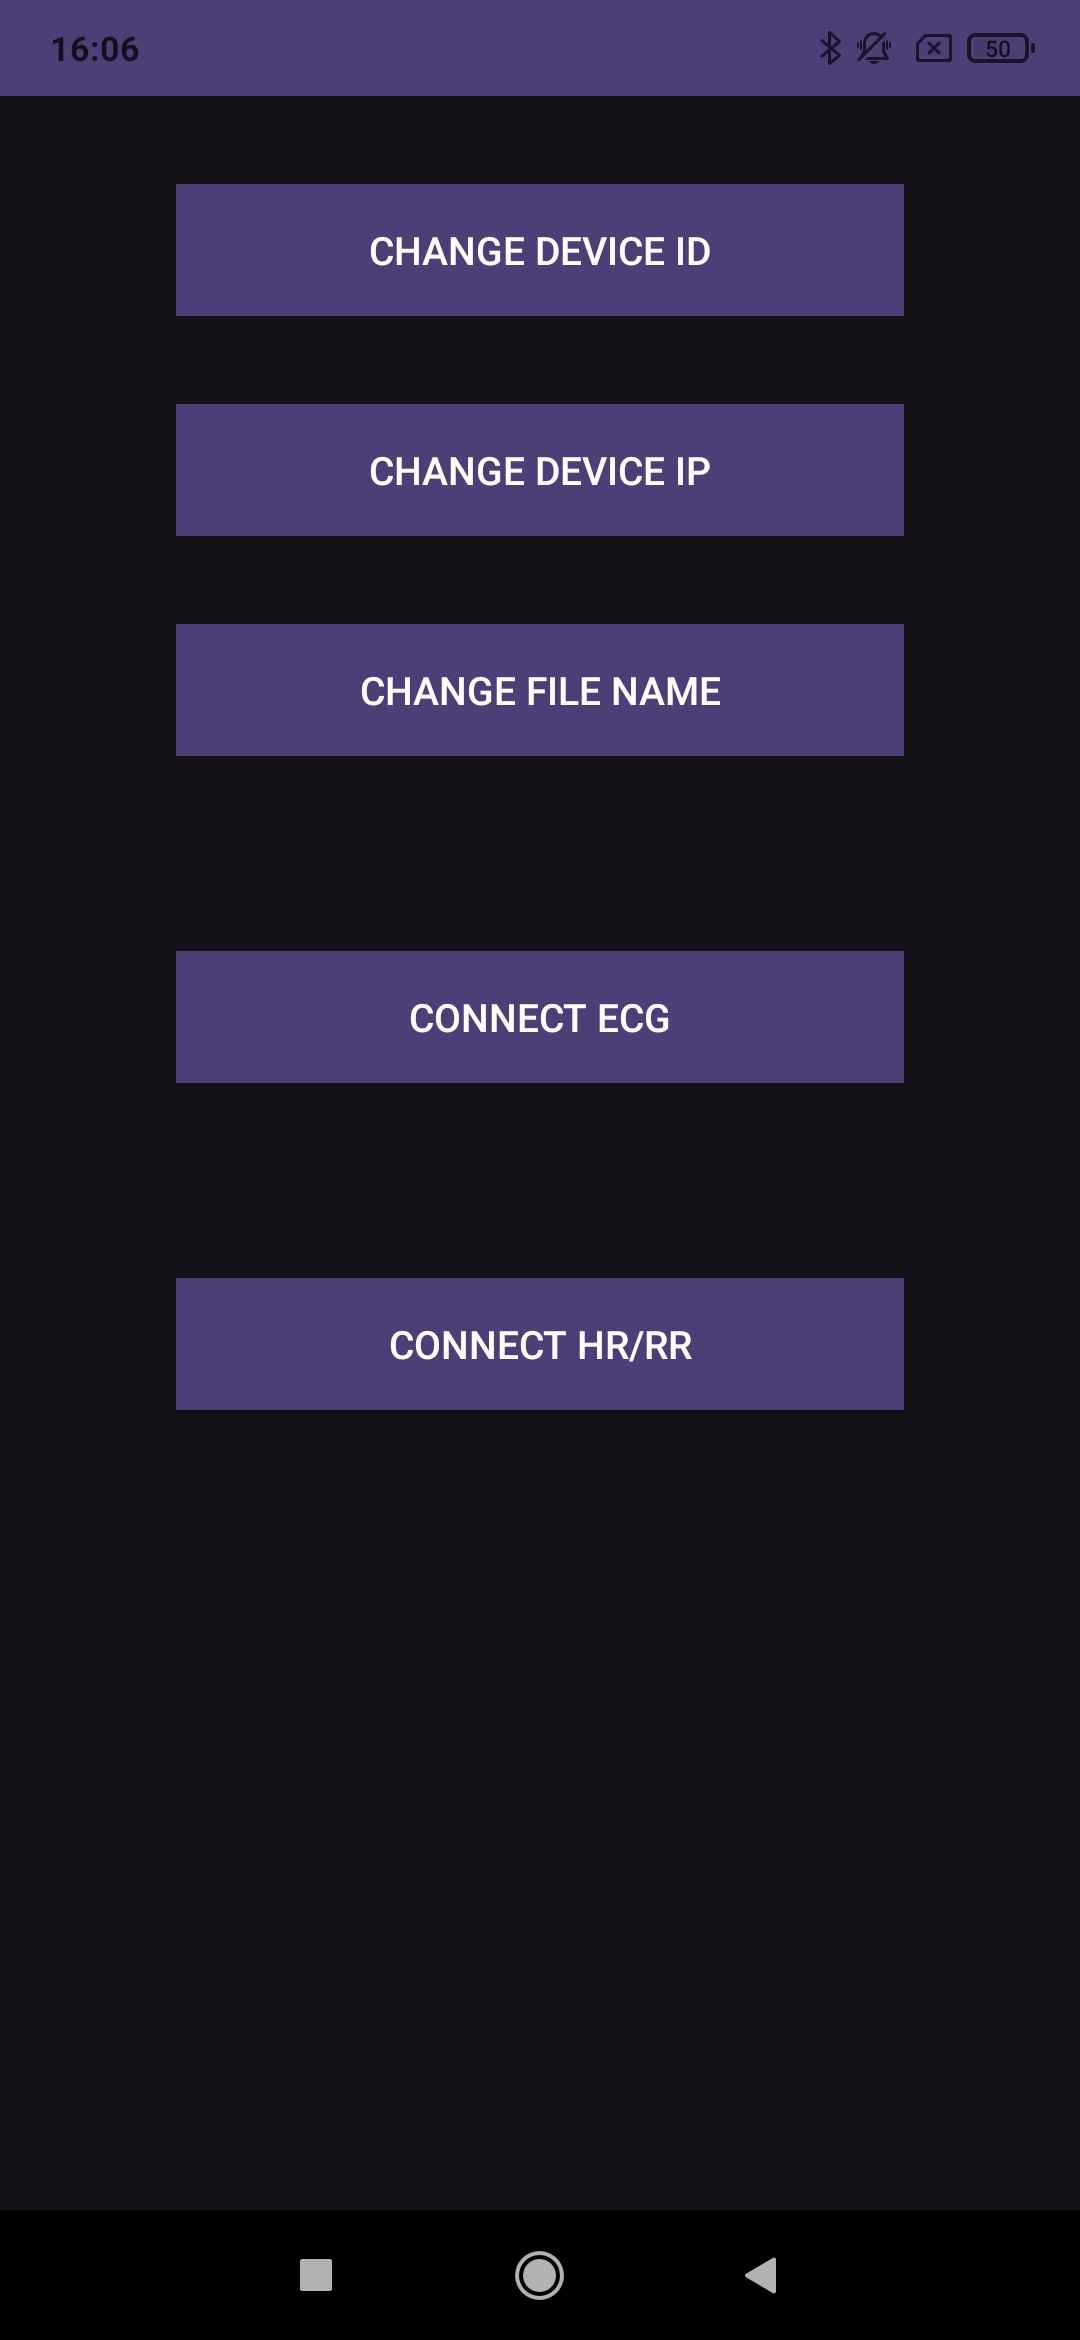
\includegraphics[width=.48\linewidth]{Rysunki/polargraphMENU.jpg}}
    \hspace{0.5cm} % Odst�p poziomy mi�dzy zdj�ciami
    \subfloat[Zak�adka analizy EKG\label{subfig:2}]
    {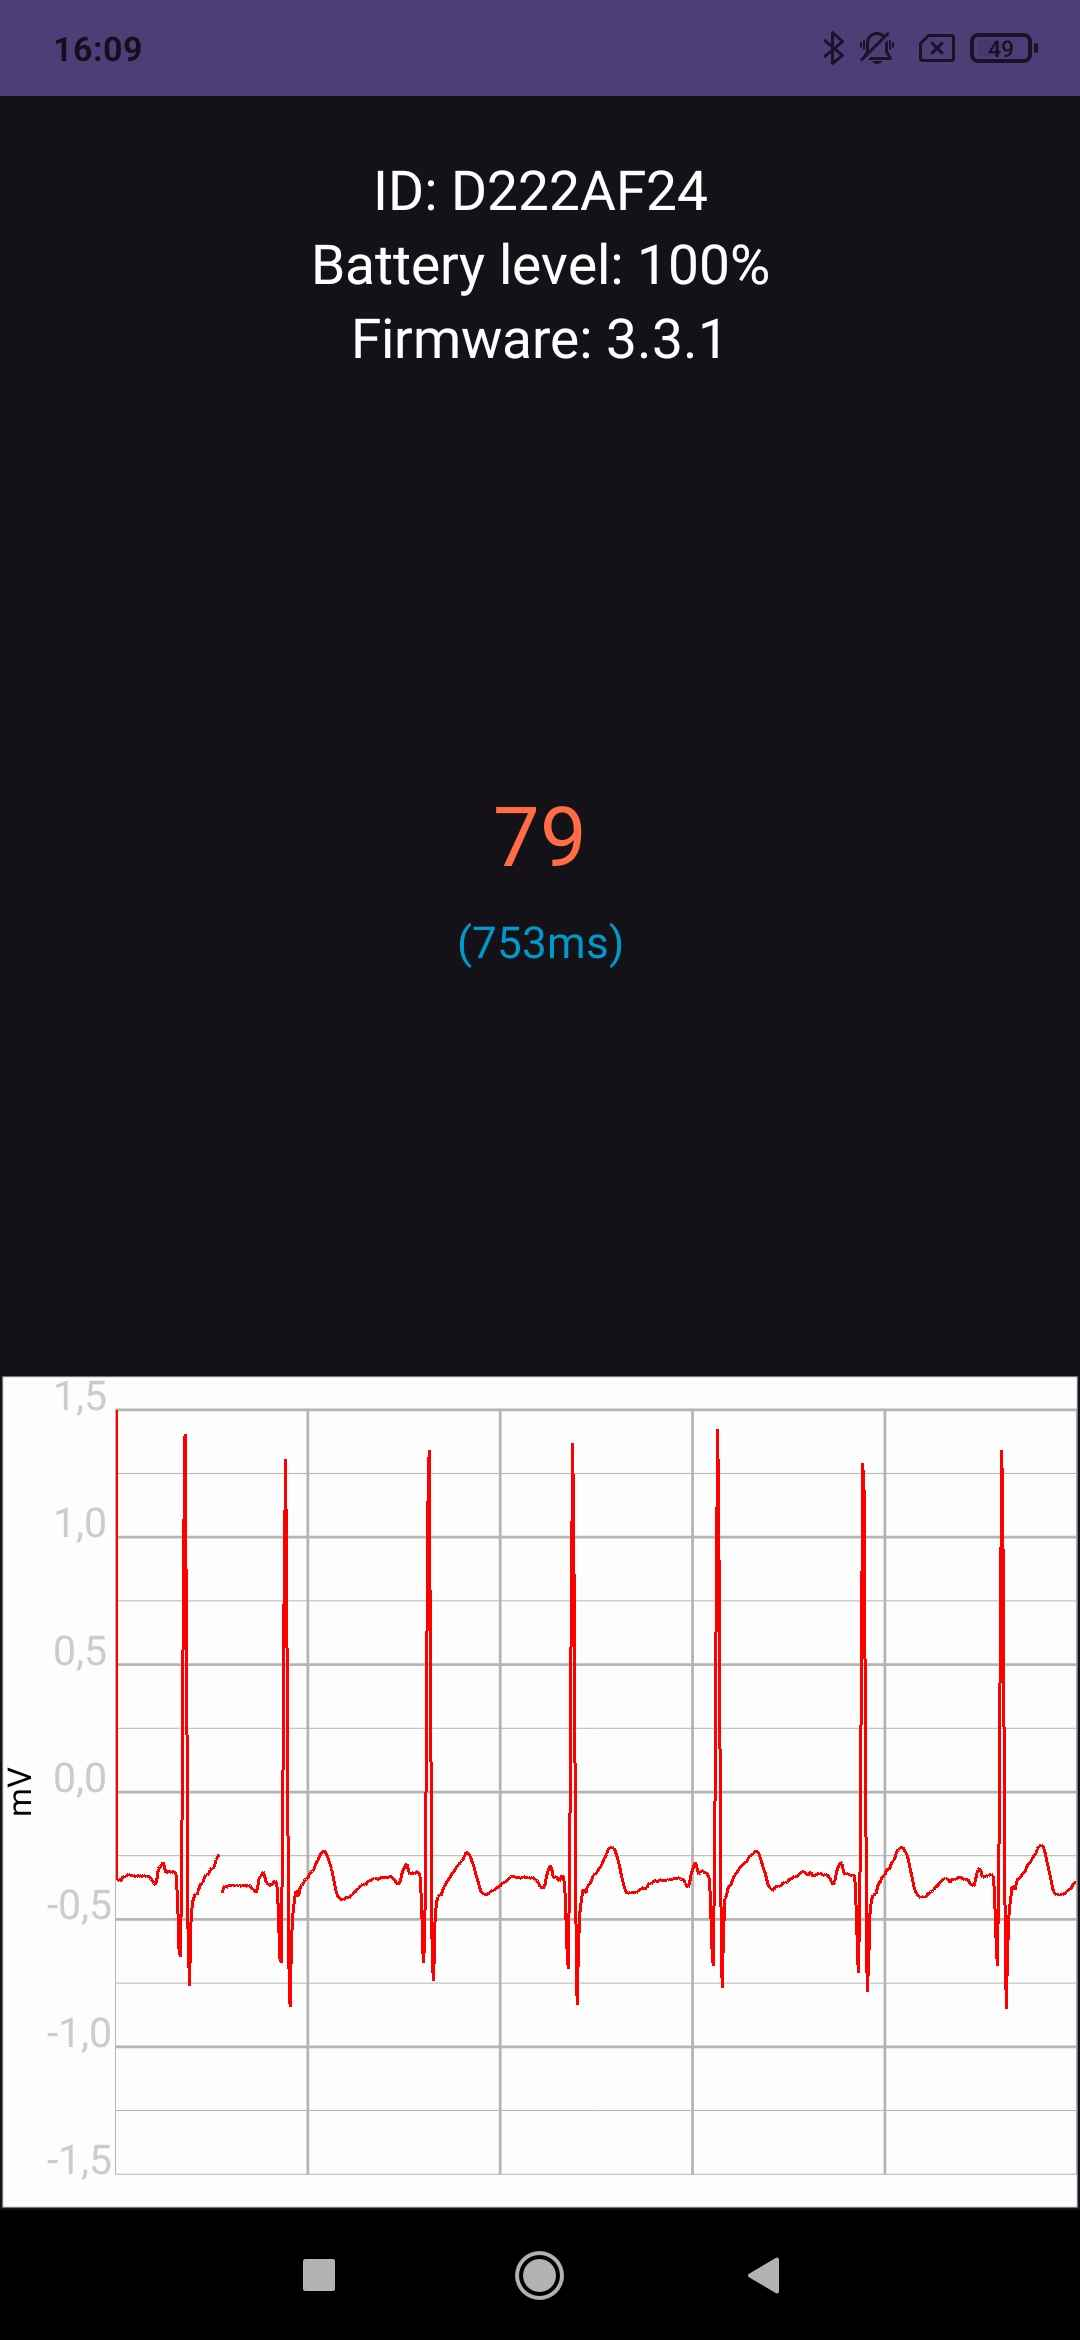
\includegraphics[width=.48\linewidth]{Rysunki/polargraph_ekg.jpg}}
    \vspace{0.5cm} % Odst�p poziomy mi�dzy zdj�ciami
    \caption{Efekt dzia�ania aplikacji do po��czenia z czujnikiem Polar H10.\label{fig:main}}
\end{figure}

\FloatBarrier

\subsection{Funkcjonalno�ci Dedykowanej Aplikacji}
Aplikacja zosta�a opracowana na podstawie przyk�adowego szkieletu dostarczonego przez producenta, kt�ry zawiera� wst�pnie zaimplementowane funkcje, takie jak: wy�wietlanie wykresu sygna�u EKG z automatycznym przesuwaniem w czasie, obliczanie i wy�wietlanie miar, takich jak czas ostatnich interwa��w RR czy t�tno, a tak�e dodatkowe informacje, np. poziom na�adowania baterii. Gotowa by�a r�wnie� logika zarz�dzania po��czeniem z czujnikiem za po�rednictwem BLE oraz odbierania pakiet�w z danymi EKG \cite{Polar-BLE-SDK}. Na potrzeby tej pracy dodano funkcjonalno�� obs�ugi po��czenia z serwerem, na kt�ry przesy�ane by�y dane EKG, przetworzone wcze�niej do postaci bajtowej zgodnie z wymaganiami okre�lonymi w kontrakcie serwera. Dodatkowo stworzono mechanizm zapisywania danych do plik�w, umo�liwiaj�cy utrwalenie zebranych pr�bek w celu ich dalszej analizy. Domy�lnie pr�bki zapisywane s� w plikach obejmuj�cych 5-minutowe interwa�y, kt�re s� oznaczane nazwami zgodnymi z aktualnym czasem. W przypadku d�u�szego pomiaru aplikacja automatycznie generuje kolejne pliki dla kolejnych 5-minutowych okres�w. Takie podej�cie minimalizuje ewentualne straty danych w przypadku utraty po��czenia z czujnikiem lub b��du zapisu do pliku. W celu usprawnienia analizy d�u�szych odcink�w sygna�u zaimplementowano funkcjonalno�� umo�liwiaj�c� po��czenie wybranych plik�w w odpowiedniej kolejno�ci. Kolejno�� ta jest okre�lana na podstawie nazw plik�w, a wynikowy plik CSV zawiera scalone dane w jednolitym formacie.

\section{Opis Paczek Danych \small{(autor: Piotr Weso�owski)}}
Funkcjonalno�ci zaimplementowane w kodzie, korzystaj� z interfejsu API Polar, aby w czasie rzeczywistym pobiera� dane z czujnika EKG. Dane s� przesy�ane w paczkach, z kt�rych ka�da zawiera oko�o 73 pr�bki. Liczba ta wynika z implementacji API producenta i jest optymalizowana pod k�tem efektywno�ci transmisji oraz niskiego op�nienia w technologii BLE. Ka�da pr�bka sk�ada si� z warto�ci potencja�u elektrycznego w mikrovoltach (\textmu{}V) (ang. \textit{Voltage}) oraz znacznika czasowego (ang. \textit{Timestamp}). Czujnik wysy�a dane sk�adaj�ce si� z timestampu, kt�ry mierzy liczb� nanosekund, jakie up�yn�y od pewnego momentu w czasie. Domy�lnie, zgodnie z UNIX, tym momentem jest 1970-01-01T00:00:00Z. Jednak w przypadku tego urz�dzenia punktem odniesienia jest 2019-01-01T00:00:00Z (599616000000000000 nanosekund). Decyzja ta wynika z ogranicze� pami�ci poprzednich modeli oraz ch�ci zachowania sp�jno�ci przez producenta \cite{Polar-BLE-SDK}.

\section{Podsumowanie \small{(autor: Piotr Weso�owski)}}
Czujnik mierzy aktywno�� elektryczn� serca, kt�ra powstaje w wyniku depolaryzacji i repolaryzacji kom�rek mi�nia sercowego podczas jego pracy. Urz�dzenie wykorzystuje dwie elektrody, kt�re rejestruj� r�nice potencja��w mi�dzy punktami na sk�rze. Napi�cia te, zwykle w mikrowoltach (\textmu{}V), s� wzmacniane, filtrowane i digitalizowane, aby stworzy� sygna� EKG. Pozyskane dane s� nast�pnie przesy�ane do serwera dzia�aj�cego na osobnej maszynie poprzez sie� i wykorzystanie protoko�u TCP/IP.


\section{Dodatkowe zbiory danych \small{(autor: Jakub Wojtalewicz)}}
W pracy, poza zbiorem danych zebranym przy u�yciu sensora Polar H10, wykorzystano r�wnie� zbiory danych pochodz�ce z zewn�trznych �r�de�. Pos�u�y�y one jako dodatkowy materia� do nauki modeli oraz weryfikacji ich skuteczno�ci w analizie sygna��w EKG. 
\subsection{MIT-BIH Arrhythmia Database \cite{MIT-BIH}}
MIT-BIH Arrhythmia Database to zbi�r danych zawieraj�cy 48 p�godzinnych zapis�w sygna�u EKG zarejestrowanych w latach 1975-1979 w szpitalu Beth Isreel w Bostonie. Dane pochodz� od 47 pacjent�w, zar�wno hospitalizowanych (oko�o 60\%) jak i ambulatoryjnych (oko�o 40\%). Nagrania zosta�y zdigitalizowane z cz�stotliwo�ci� pr�bkowania 360 Hz, z 11-bitow� rozdzielczo�ci� w zakresie 10 mV. Dla ka�dego sygna�u dost�pne s� adnotacje opracowane przez dw�ch lub wi�cej kardiolog�w, kt�re sumarycznie sk�adaj� sie na oko�o 110 000 oznaczonych uderze� serca.

\subsection{MIT-BIH Noise Stress Test Database \cite{MIT-BIH-Noise}}
MIT-BIH Noise Stress Test Database to zbi�r danych stworzony w celu oceny odporno�ci algorytm�w analizy EKG na r�ne rodzaje zak��ce�. Zawiera 12 p�godzinnych zapis�w sygna�u EKG oraz 3 p�godzinne zapisy zak��ce� typowych dla ambulatoryjnych rejestracji EKG. Zak��cenia te obejmuj� dryft linii bazowej (baseline wander), artefakty mi�niowe (EMG) oraz artefakty ruchu elektrod. Nagrania powsta�y poprzez dodanie zak��ce� do dw�ch czystych zapis�w EKG z pierwotnego zbioru MIT-BIH Arrhythmia Database (nagrania 118 i 119).

Zak��cenia zosta�y wprowadzone w segmentach dwuminutowych, przeplatanych fragmentami czystego sygna�u, z r�nymi stosunkami sygna�u do szumu (SNR). Dla ka�dego nagrania dost�pne s� prawid�owe adnotacje pochodz�ce z oryginalnych czystych zapis�w.
\chapter{Implementacja systemu}


\section{Analiza faz cyklu oddechowego na podstawie wykresu t�tna}

\subsection{Wprowadzenie}
System zaprojektowano do okre�lania faz oddechu na podstawie zmian w t�tnie. Silny efekt RSA powodowa� wzrost mocy sygna�u w tym samym pa�mie cz�stotliwo�ci, co dominuj�ca cz�stotliwo�� rytmu oddechowego w danej pr�bce. Na przyk�ad dla osoby oddychaj�cej w tempie 12 cykli na minut� (0.2 Hz), wysoki poziom mocy sygna�u w tej cz�stotliwo�ci wskazywa� na intensywny efekt RSA. 

Aby precyzyjnie okre�li� fazy oddechu, konieczne by�o wykrywanie lokalnych ekstrem�w w sygnale t�tna. Minima odpowiada�y pocz�tkom wdechu, a maksima pocz�tkom wydechu.

\subsection{Przetwarzanie sygna�u za pomoc� filtru pasmowego}
W celu identyfikacji tych zmian, sygna� t�tna zosta� przetworzony za pomoc� cyfrowego filtru pasmowego w konfiguracji bez przesuni�cia fazowego, wykorzystuj�c funkcj� \texttt{filtfilt} z biblioteki \texttt{scipy.signal}. Filtr pasmowy zosta� zoptymalizowany pod k�tem cz�stotliwo�ci oddechu  osoby badanej. Zastosowano filtr Butterwortha 4. rz�du, zapewniaj�cy odpowiedni� r�wnowag� mi�dzy stromo�ci� charakterystyki a stabilno�ci� przetwarzanego sygna�u. Nale�y jednak zauwa�y�, �e zastosowanie filtra 4. rz�du powoduje znacz�ce op�nienie w przetwarzaniu sygna�u. W konsekwencji prawid�owe dzia�anie algorytmu wymaga uwzgl�dnienia co najmniej 28 pr�bek interwa��w RR, aby unikn�� zniekszta�ce� wynikaj�cych z niewystarczaj�cego buforowania danych.

Filtr Butterwortha w konfiguracji pasmowo-przepustowej przepuszcza� tylko cz�stotliwo�ci w zakresie okre�lonym parametrami \textit{low} i \textit{high}, znormalizowanym wzgl�dem cz�stotliwo�ci Nyquista (65 Hz dla cz�stotliwo�ci pr�bkowania 130 Hz). 

\subsection{Dob�r parametr�w filtru}
Na podstawie literatury oraz analizy heurystycznej ustalono, �e najlepsze wyniki mo�na uzyska�, stosuj�c filtr przepuszczaj�cy cz�stotliwo�ci w zakresie od po�owy cz�stotliwo�ci centralnej do dwukrotno�ci tej cz�stotliwo�ci. Cz�stotliwo�� centraln� definiuje si� jako warto��, dla kt�rej analizowany sygna� wykazuje najwi�ksz� moc.

Przyk�adowo, dla osoby oddychaj�cej z cz�stotliwo�ci� oko�o 6 oddech�w na minut� (co odpowiada 0,1 Hz), optymalne pasmo filtra wynosi od 0,05 Hz do 0,2 Hz. W celu uzyskania takich ustawie�, parametry filtra \textit{low} i \textit{high} nale�y ustawi� odpowiednio na warto�ci 0,05 Hz i 0,2 Hz. Tak dobrany zakres pozwala na uzyskanie wyra�nych lokalnych ekstrem�w w przefiltrowanym sygnale t�tna, co umo�liwia precyzyjne okre�lenie faz cyklu oddechowego.

Filtracja dolnych warto�ci (poni�ej 0,05 Hz) pozwala odfiltrowa� powolne wahania sygna�u, takie jak wp�yw zmian pozycji cia�a, artefakty ruchowe o niskiej cz�stotliwo�ci lub d�ugoterminowe trendy w sygnale. Z kolei odci�cie g�rnych warto�ci (powy�ej 0,2 Hz) eliminuje zak��cenia wynikaj�ce z takich czynnik�w jak szum o wysokiej cz�stotliwo�ci, szybkie artefakty ruchowe lub sk�adowe zwi�zane z wysokocz�stotliwo�ciowymi procesami fizjologicznymi, kt�re nie s� zwi�zane z oddechem.

Opisywany algorytm wykazywa� jednak pewne ograniczenia, szczeg�lnie w przypadku szybszych oddech�w (o cz�stotliwo�ci powy�ej 0,25 Hz). Ponadto, w obecnej implementacji wymaga� on filtrowania ca�ego sygna�u, co w trybie rzeczywistym lub podczas analizy du�ych pr�bek danych, znacz�co zwi�ksza�o obci��enie obliczeniowe.

\subsection{Detekcja szczyt�w lokalnych i analiza faz oddechowych}

Do identyfikacji lokalnych szczyt�w w sygnale wykorzystano funkcj� \texttt{find\_peaks} z biblioteki \texttt{scipy.signal}. W parametrach funkcji zdefiniowano pr�g (\textit{threshold}) jako �redni� warto�� przefiltrowanego sygna�u powi�kszon� o 10\% odchylenia standardowego, co okre�la�o minimalny poziom, powy�ej kt�rego poszukiwano szczyt�w. Dodatkowo, ustawiono minimaln� odleg�o�� (\textit{distance}) mi�dzy kolejnymi szczytami jako liczb� pr�bek odpowiadaj�c� czasowi trwania po�owy jednego cyklu oddechowego. 

W celu detekcji do�k�w sygna� zosta� odwr�cony poprzez zmian� znaku wszystkich pr�bek, a nast�pnie zastosowano te same procedury co w przypadku wykrywania szczyt�w. Proces detekcji uzupe�niono o autorski algorytm korekcji pozycji wykrytych ekstrem�w wzgl�dem sygna�u nieprzefiltrowanego, co opisano szczeg�owo w Rozdziale \ref{P-Tomkins}.

Wyznaczone ekstrema oznaczono na wykresie t�tna kolorami: minima jako zielone punkty, a maksima jako czerwone punkty. Na podstawie wykrytych ekstrem�w zaimplementowano algorytm identyfikuj�cy momenty trwania poszczeg�lnych wdech�w i wydech�w. Wdech zdefiniowano jako fragment sygna�u rozpoczynaj�cy si� w minimum wykresu t�tna i ko�cz�cy si� w kolejnym maksimum, pod warunkiem, �e pomi�dzy tymi punktami nie wyst�powa�y dodatkowe minima. Analogicznie, wydech okre�lono jako fragment rozpoczynaj�cy si� w maksimum i ko�cz�cy w kolejnym minimum.

Przyj�te podej�cie zapewnia odporno�� na sytuacje, w kt�rych algorytm nie wykry�by niekt�rych minim�w lub maksim�w. Na przyk�ad brak detekcji ko�ca fazy oddechowej m�g�by prowadzi� do sztucznego wyd�u�enia czasu jej trwania. Dzi�ki zdefiniowanym regu�om minimalizowano wp�yw takich przypadk�w na wyniki analizy.

Na podstawie wykrytych wdech�w i wydech�w obliczono wska�nik RSA Index � kluczow� miar� opisuj�c� si�� efektu RSA. Wska�nik ten okre�la �redni� r�nic� w d�ugo�ci interwa�u RR pomi�dzy pocz�tkiem a ko�cem zar�wno wdechu, jak i wydechu.



\subsection{Przyk�ad zastosowania algorytmu}
Na Rys. \ref{fig/oddechy} przedstawiono wyniki analizy sygna�u EKG zarejestrowanego na odcinku 118 sekund, podczas kt�rego osoba oddycha�a ze sta�� cz�stotliwo�ci� 0,07 Hz (�rednio 14 sekund na cykl oddechowy). Wykresy zosta�y wygenerowane przy u�yciu opisywanej aplikacji i uporz�dkowane w czterech rz�dach:

\begin{figure}[ht]
    \centering
    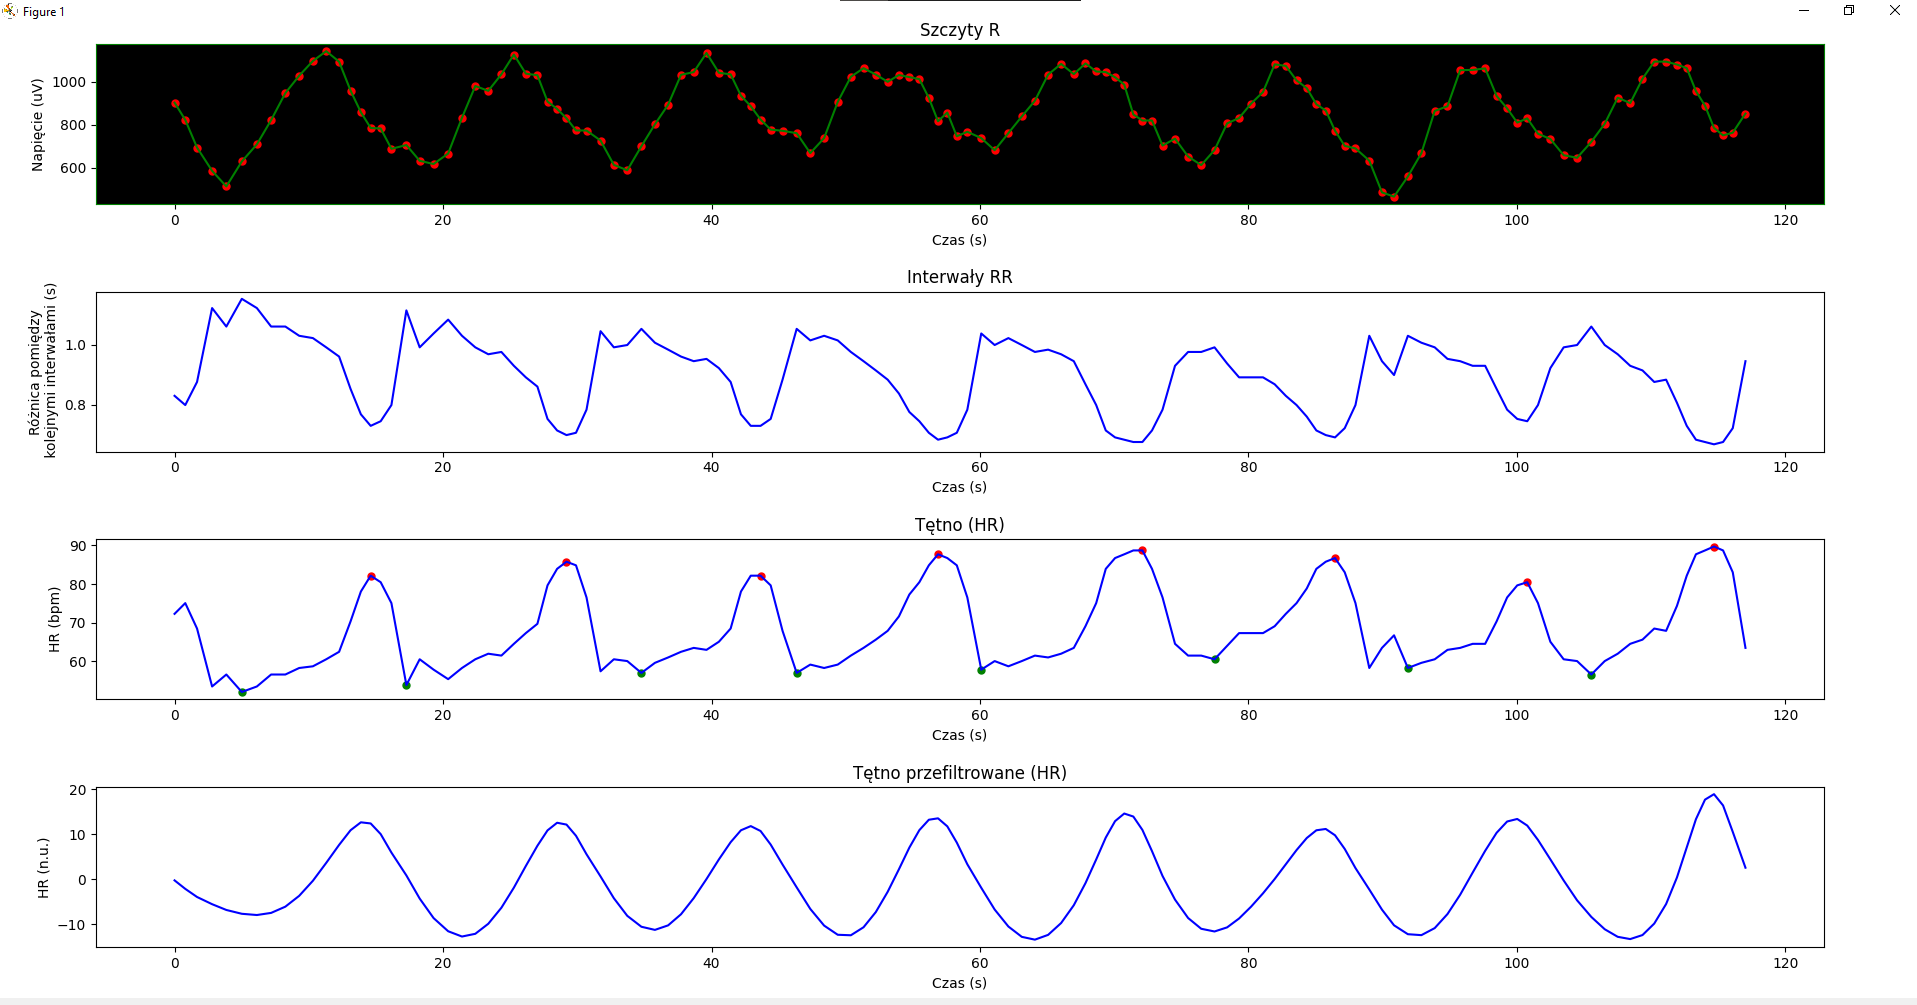
\includegraphics[width=\textwidth]{Rysunki/oddechy.png}
    \caption{Analiza sygna�u EKG: wykryte szczyty R, r�nice interwa��w RR, przebieg t�tna i jego przefiltrowany sygna�.}
    \label{fig/oddechy}
\end{figure}

\FloatBarrier

\begin{itemize}
    \item Pierwszy rz�d: Warto�ci napi�cia (w \textmu{}V) dla wykrytych szczyt�w R w czasie, wyznaczone za pomoc� algorytmu Pan-Tompkinsa.
    \item Drugi rz�d: R�nice mi�dzy kolejnymi interwa�ami RR (w sekundach) w funkcji czasu.
    \item Trzeci rz�d: Przebieg t�tna (w uderzeniach na minut�) z zaznaczonymi minimami i maksimami zgodnie z opisanymi kryteriami.
    \item Czwarty rz�d: Przefiltrowany sygna� t�tna (w jednostkach znormalizowanych) w funkcji czasu.
\end{itemize}


\subsection{Podsumowanie wynik�w}
Na podstawie analizy sygna�u aplikacja wyznaczy�a nast�puj�ce miary charakterystyczne:
\begin{itemize}
    \item �redni czas trwania wdechu: 9,99 s,
    \item �redni czas trwania wydechu: 4,25 s,
    \item {RSA Index}: Maksymalna r�nica d�ugo�ci interwa��w RR w ca�ym sygnale wynosi�a 0,48 s,
    \item {Mean RR Interval Difference}: �rednia r�nica d�ugo�ci interwa��w RR mi�dzy pocz�tkiem a ko�cem faz oddechu wynosi�a 0,35 s,
    \item �rednia d�ugo�� pe�nego cyklu oddechowego: 14,24 s.
\end{itemize}


\section{Analiza sygna�u EKG za pomoc� transformacji Fouriera}

\subsection{Interpolacja i spe�nienie warunku Nyquista}
W celu analizy sygna�u EKG przy u�yciu szybkiej transformacji Fouriera (FFT) obejmuj�cej cz�stotliwo�ci w zakresie 0,04�0,4 Hz, konieczne by�o przekszta�cenie nier�wnomiernie pr�bkowanego sygna�u RR w r�wnomierny. W tym celu zastosowano interpolacj� liniow� interwa��w RR z cz�stotliwo�ci� pr�bkowania 4 Hz. Dzi�ki temu spe�niono warunek Nyquista, poniewa� najwi�ksza analizowana cz�stotliwo�� (0,4 Hz) le�y poni�ej po�owy cz�stotliwo�ci pr�bkowania (2 Hz).

\subsection{Przygotowanie sygna�u do analizy}
Przed wykonaniem transformacji na sygna� na�o�ono okno Hanninga. Okno to redukuje amplitudy na pocz�tku i ko�cu sygna�u, co pozwala na wyg�adzenie danych i minimalizacj� efekt�w nieci�g�o�ci. Nast�pnie wykonano dyskretn� transformacj� Fouriera, kt�ra przekszta�ca sygna� z dziedziny czasu do dziedziny cz�stotliwo�ci. 

W wyniku FFT uzyskano dwa wektory:
\begin{itemize}
    \item \texttt{fft\_result} � zawieraj�cy informacje o amplitudach i fazach sk�adowych cz�stotliwo�ciowych,
    \item \texttt{freqs} � wskazuj�cy cz�stotliwo�ci odpowiadaj�ce poszczeg�lnym warto�ciom w \texttt{fft\_result}.
\end{itemize}

\subsection{Obliczanie mocy w pasmach cz�stotliwo�ci}
Moc sygna�u w okre�lonych pasmach, takich jak LF czy HF, obliczono jako ca�k� z kwadratu modu�u amplitud \(|FFT|^2\) w odpowiednim przedziale cz�stotliwo�ci. W praktyce odpowiada to sumie warto�ci mocy przypisanych do tych cz�stotliwo�ci:
\[
\text{Power} = \int_{f_1}^{f_2} |FFT(f)|^2 df.
\]
Dzi�ki temu mo�liwe by�o zwizualizowanie mocy w ca�ym zakresie cz�stotliwo�ci, jak r�wnie� w wybranych pasmach, a tak�e obliczanie stosunku LF/HF. 

\subsection{Ograniczenia i uwagi dotycz�ce metody FFT}
Transformacja FFT wymaga dost�pu do ca�ego sygna�u, co oznacza, �e analiza w czasie rzeczywistym jest obarczona op�nieniem wynikaj�cym z czasu potrzebnego na zebranie danych i przeprowadzenie oblicze�.

\subsection{Wyniki analizy FFT}
Poni�ej zamieszczono wynik szybkiej transformaty Fouriera kt�ry zosta� wygenerowany przy u�yciu modu�u implementowanego w ramach stworzonej aplikacji. Na wykresie przedstawiono widmow� g�sto�� mocy (Power Spectral Density, PSD), wyra�on� w jednostkach \([ms^2/Hz]\), w dziedzinie cz�stotliwo�ci. Analiza zosta�a wykonana na sygnale z 5-minutowego badania przeprowadzonego podczas snu.


\subsection{Wizualizacja wynik�w}
Na wykresie \ref{fig:fft_psd}, uwidoczniono warto�ci mocy w poszczeg�lnych pasmach cz�stotliwo�ci: LF, HF oraz stosunek LF/HF. Zauwa�alna jest dominuj�ca moc w pa�mie ULF (Ultra-Low Frequency, poni�ej 0,003 Hz).
\begin{figure}[ht]
    \centering
    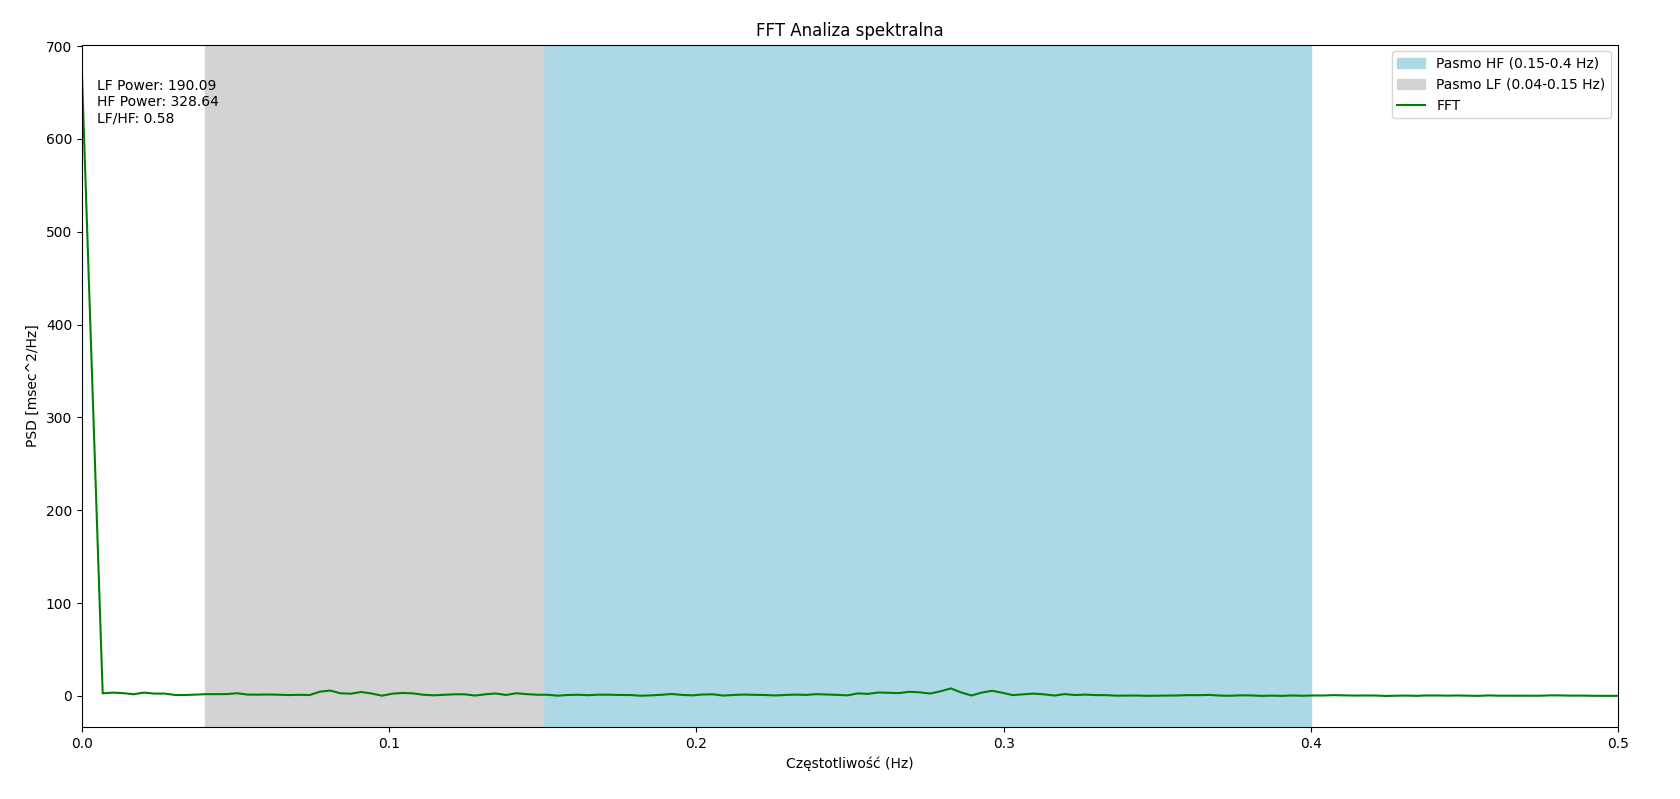
\includegraphics[width=\textwidth]{Rysunki/fftFAR.png}
    \caption{Widmowa g�sto�� mocy (PSD) dla 5-minutowego badania.}
    \label{fig:fft_psd}
\end{figure}

\FloatBarrier

Na wykresie \ref{fig:fft_zoomed}, b�d�cym przybli�eniem rozk�adu g�sto�ci mocy tego samego sygna�u, widoczne s� lokalne wzrosty mocy w pa�mie cz�stotliwo�ci \(0,28\ \text{Hz}\) (HF) oraz mniejszy, ale wyra�ny wzrost dla cz�stotliwo�ci \(0,09\ \text{Hz}\) (LF).
\begin{figure}[ht]
    \centering
    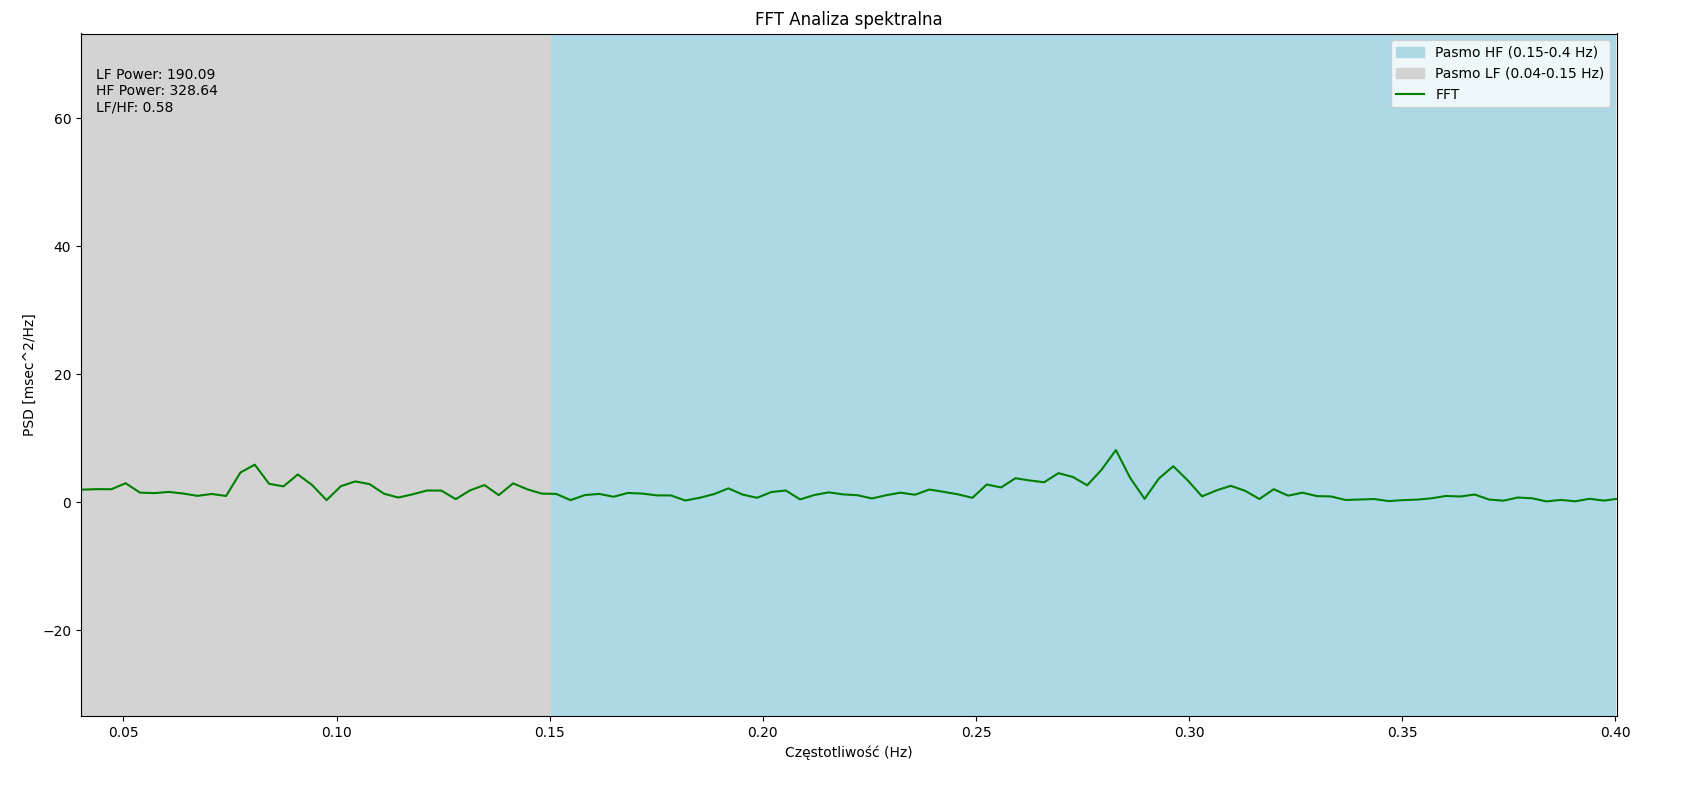
\includegraphics[width=\textwidth]{Rysunki/fftCLOSE.png}
    \caption{Przybli�enie rozk�adu g�sto�ci mocy w pasmach LF i HF.}
    \label{fig:fft_zoomed}
\end{figure}

\FloatBarrier


\section{Analiza czasowo-cz�stotliwo�ciowa}

W analizie czasowo-cz�stotliwo�ciowej, r�wnie� zastosowano interpolacj� interwa��w RR do cz�stotliwo�ci 4 Hz, aby zapewni� r�wnomierne pr�bkowanie sygna�u. Do analizy wykorzystano sinusoidaln� falk� Morleta, kt�ra jest szczeg�lnie dobrze dopasowana do sygna��w harmonicznych, takich jak RSA. 

\subsection{Parametry analizy falkowej}
Falka Morleta, zaimplementowana przy u�yciu biblioteki PyWavelets, umo�liwia precyzyjn� analiz� w interesuj�cym zakresie cz�stotliwo�ci. Kluczowe parametry falki zosta�y dostosowane w nast�puj�cy spos�b:
\begin{itemize}
    \item \textbf{Szeroko�� pasma:} \(B = 15\), co dzi�ki stosunkowo wysokiej warto�ci zwi�ksza precyzj� w dziedzinie cz�stotliwo�ci, jednocze�nie zachowuj�c odpowiedni kompromis z rozdzielczo�ci� czasow�,
    \item \textbf{Cz�stotliwo�� centralna:} \(C = 0.22\), kt�ra skupia energi� falki na kluczowym dla analizy przedziale cz�stotliwo�ci.
\end{itemize}

\subsection{Wyznaczanie mocy sygna�u}
Stworzono funkcj� obliczaj�c� parametr \textit{scales}, czyli poziomy skalowania funkcji falkowej, odpowiadaj�ce analizowanemu zakresowi cz�stotliwo�ci (0,03�0,5 Hz). Parametr ten pozwala� dostosowa� analiz� do wybranych cz�stotliwo�ci, umo�liwiaj�c transformacj� falkow� sygna�u i uzyskanie wsp�czynnik�w (\textit{coefficients}), kt�re wskazuj�, jak mocno sygna� pasuje do falki w danym momencie i dla danej skali. Na tej podstawie liczona by�a moc sygna�u jako suma kwadrat�w amplitud:
\[
|C(a,b)|^2,
\]
co pozwala�o wizualizowa� zmiany mocy na skalogramie.

\subsection{Problemy brzegowe i wizualizacja wynik�w}
Zawy�one warto�ci mocy na kra�cach dziedziny czasowej wynika�y z efekt�w brzegowych � falka cz�ciowo wykracza�a poza sygna�, co prowadzi�o do zniekszta�ce�. W celu poprawy widoczno�ci zmian na skalogramie przedstawiono zlogarytmowan� moc w formie kolorowej mapy w uk�adzie czas-cz�stotliwo��.

Program umo�liwia r�wnie� obliczanie mocy sygna�u w wybranych pasmach cz�stotliwo�ci (np. LF lub HF) oraz wizualizacj� ich zmian, a tak�e ich stosunku \textit{LF/HF} w czasie. Wszystkie te funkcjonalno�ci dzia�aj� zar�wno podczas analizy sygna�u w czasie rzeczywistym, jak i podczas analizy danych wczytywanych z pliku.

Ze wzgl�du na specyfik� dzia�ania transformacji falkowej, kt�ra mo�e generowa� zniekszta�cenia na granicach sygna�u w dziedzinie czasowej, moc obliczana jest dla ca�ego zakresu czasowego jednocze�nie. Mo�e to prowadzi� do op�nie�, zw�aszcza w przypadku analizy w czasie rzeczywistym lub przetwarzania sygna��w o du�ej d�ugo�ci.

\subsection{Wyniki analizy}
Na zamieszczonym obrazie przeanalizowano t� sam� 5-minutow� pr�bk� zarejestrowan� podczas snu, kt�ra by�a om�wiona w rozdziale dotycz�cym implementacji FFT. Przedstawione wykresy, wygenerowane za pomoc� aplikacji stworzonej w ramach niniejszej pracy, obrazuj�:
\begin{itemize}
    \item {Pierwszy rz�d:} Skalogram, na kt�rym logarytmowana moc sygna�u jest zobrazowana kolorami zgodnie z legend�, w zale�no�ci od cz�stotliwo�ci (o� Y) i czasu (o� X).
    \item {Drugi rz�d:} Zmiany mocy w czasie dla pasm HF i LF, oznaczone zgodnie z opisami w legendzie.
    \item {Trzeci rz�d:} Stosunek mocy pasm HF do LF w funkcji czasu.
\end{itemize}

Warto zwr�ci� uwag� na zawy�one warto�ci mocy na kra�cach analizowanego okresu.



\begin{figure}[ht]
    \centering
    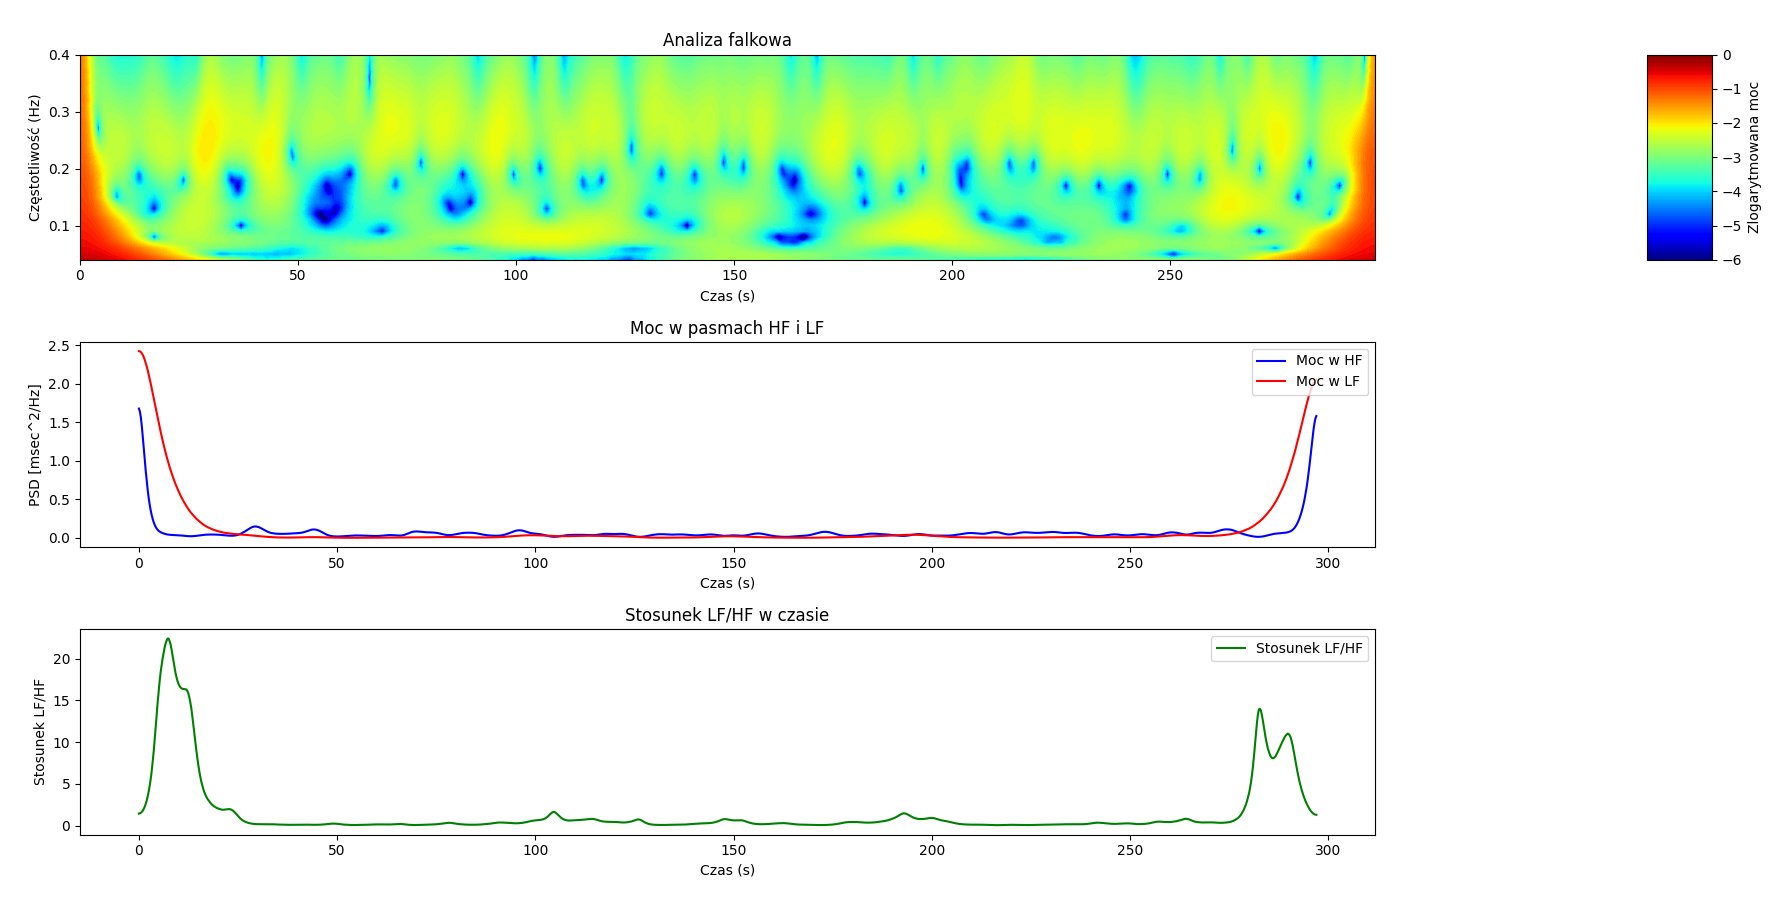
\includegraphics[width=\textwidth]{Rysunki/waveFAR.png}
    \caption{Wyniki analizy czasowo-cz�stotliwo�ciowej dla 5-minutowej pr�bki sygna�u.}

    \label{fig:wave_normal}
\end{figure}

\FloatBarrier

Na kolejnym wycinku zaprezentowano te same wykresy, przybli�one do zakresu od 30. do 270. sekundy. Przybli�enie to pozwala wyeliminowa� zniekszta�cenia spowodowane efektem brzegowym analizy falkowej, co zapewnia bardziej precyzyjn� wizualizacj� danych. W analizowanym zakresie zauwa�alna jest dominacja mocy w przedziale cz�stotliwo�ci \(0,2\text{--}0,3\ \text{Hz}\) (pasmo HF) w stosunku do pasma LF. Zale�no�� t� wyra�nie pokazuj� zar�wno skalogram, jak i wykresy mocy obu pasm oraz ich stosunku \ref{fig:wave_zoomed}.

\begin{figure}[ht]
    \centering
    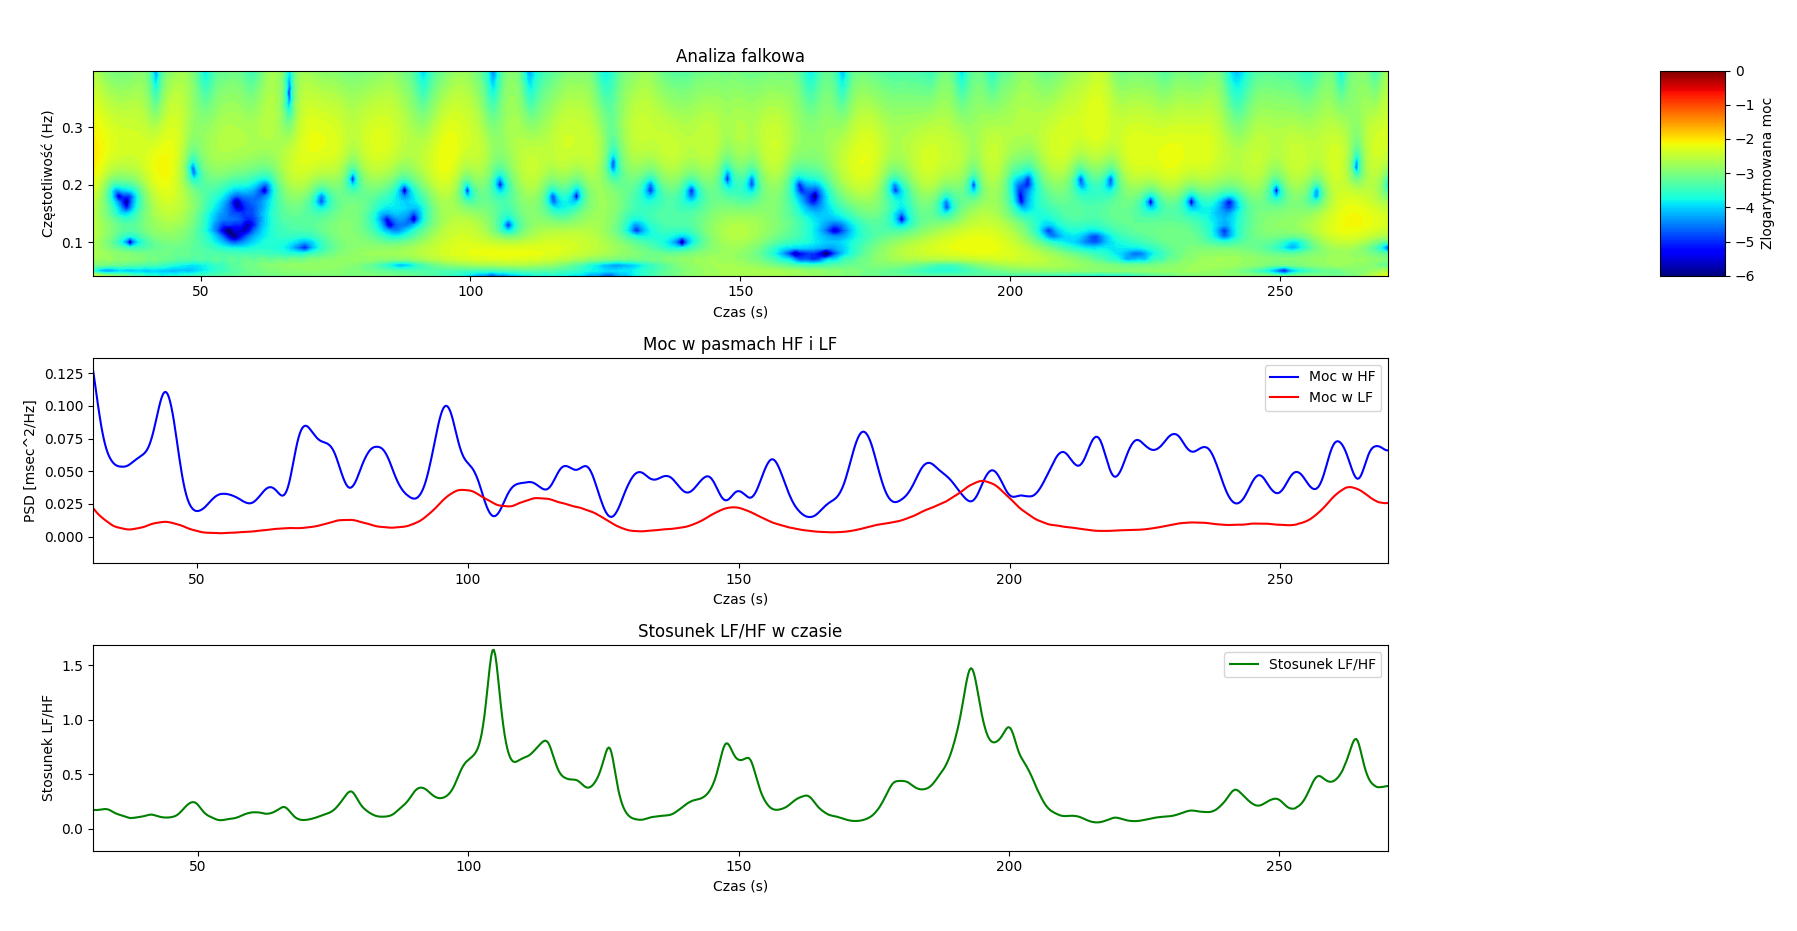
\includegraphics[width=\textwidth]{Rysunki/waveCLOSE.png}
    \caption{Przybli�enie analizy czasowo-cz�stotliwo�ciowej w ograniczonym zakresie czasu, bez widocznych efekt�w brzegowych.}
    \label{fig:wave_zoomed}
\end{figure}

\FloatBarrier

\section{Implementacja i Wizualizacja �redniej Krocz�cej}

Na podstawie wykresu \ref{fig:wavePORANEK}, przedstawiaj�cego rozk�ad mocy w dziedzinie czasu i cz�stotliwo�ci, wyznaczonego na podstawie sygna�u EKG za pomoc� analizy falkowej dla okresu 3,5 godziny, zostanie opisana implementacja i wizualizacja �redniej krocz�cej.

\begin{figure}[ht]
    \centering
    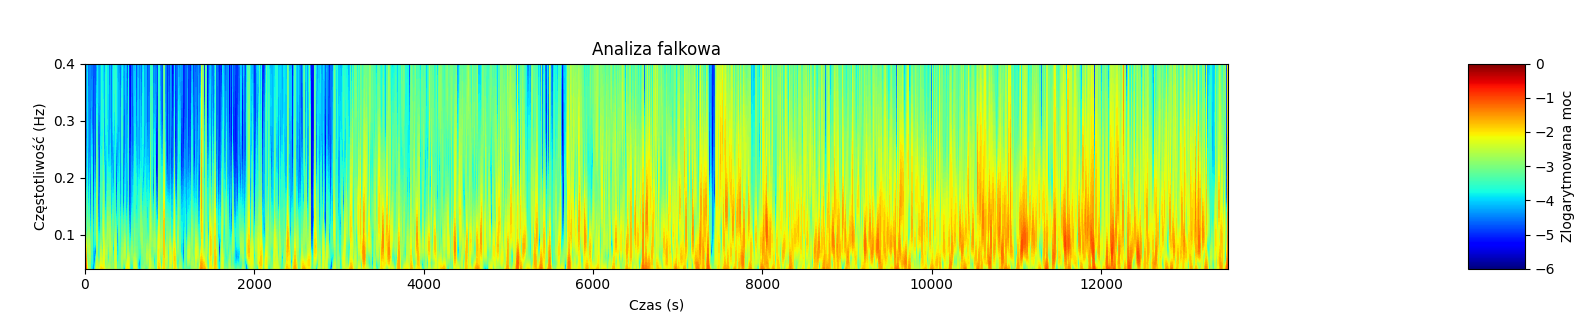
\includegraphics[width=\textwidth]{Rysunki/wavePORANEK.png}
    \caption{Skalogram przedstawiaj�cy rozk�ad mocy w dziedzinie czasu i cz�stotliwo�ci dla sygna�u EKG uzyskany za pomoc� analizy falkowej.}
    \label{fig:wavePORANEK}
\end{figure}

\FloatBarrier

W przypadku analizy mocy w pasmach LF i HF oraz ich stosunku w tak d�ugim przedziale czasowym, wykres tych warto�ci mo�e by� ma�o czytelny z uwagi na du�� zmienno�� mocy w poszczeg�lnych pasmach. W takich sytuacjach, gdy chcemy zobrazowa� globalne trendy, warto zastosowa� metod� statystyczn�, jak� jest �rednia krocz�ca. Na rysunku \ref{fig:lf_avg} przedstawiono moc w pa�mie LF dla analizowanego sygna�u.

\begin{figure}[ht]
    \centering
    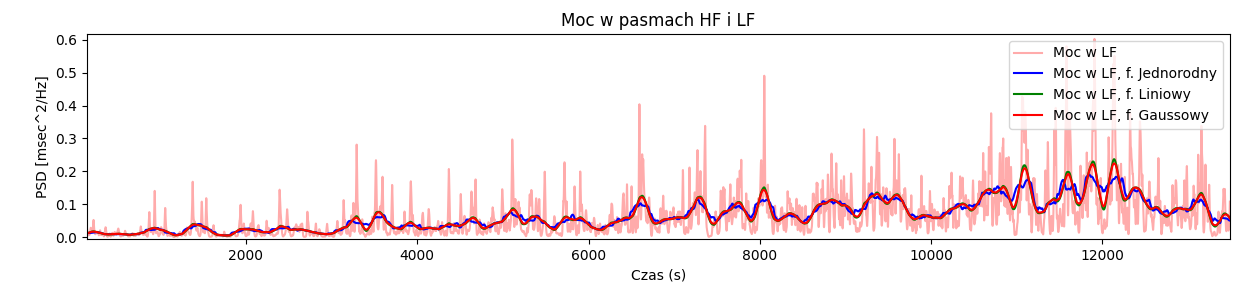
\includegraphics[width=\textwidth]{Rysunki/lf_avg.png}
    \caption{Zastosowanie r�nych metod �redniej krocz�cej do wyg�adzania mocy w pa�mie LF, przedstawiaj�ce ich wp�yw na odwzorowanie trend�w w d�u�szej perspektywie czasowej.}
    \label{fig:lf_avg}
\end{figure}

\FloatBarrier

Subteln�, r�ow� lini� zilustrowano wykres mocy w pa�mie LF z dok�adno�ci� do 0,25 sekundy \ref{fig:lf_avg} . Ze wzgl�du na du�e wahania mocy w kr�tkich odst�pach czasu, analiza tego wykresu w d�u�szej perspektywie jest trudna. Dlatego liniami o r�nych kolorach zaprezentowano zastosowanie centralnej �redniej krocz�cej dla okna o rozmiarze 900 sekund (15 minut). Linie przedstawiaj�:
\begin{itemize}
    \item �redni� jednorodn� (kolor niebieski),
    \item �redni� liniow� (kolor zielony),
    \item �redni� gaussowsk� (kolor czerwony).
\end{itemize}

W d�u�szym przedziale czasowym wszystkie te �rednie wykazuj� zbli�one warto�ci, jednak po zmniejszeniu skali mo�na zaobserwowa� subtelne r�nice, co ilustruje wykres \ref{fig:lf_compare_avg}:

\begin{figure}[ht]
    \centering
    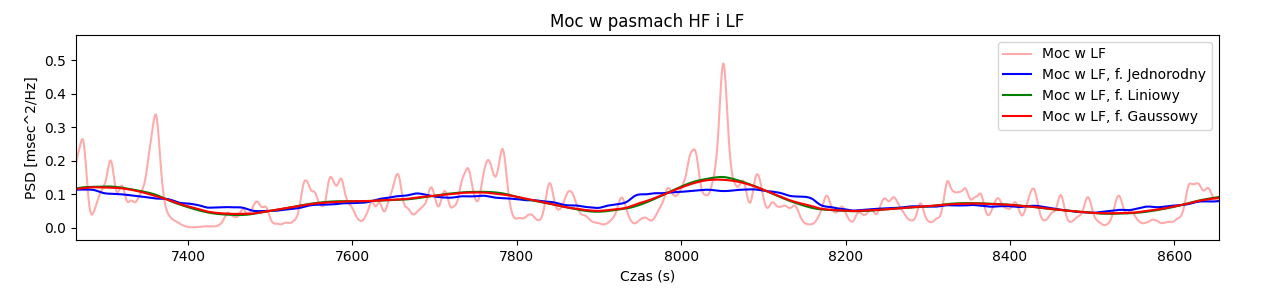
\includegraphics[width=\textwidth]{Rysunki/lf_compare_avg.png}
    \caption{R�nice w wyg�adzaniu mocy w pa�mie LF dla metod jednorodnej, liniowej i gaussowskiej, przy mniejszej skali czasowej.}
    \label{fig:lf_compare_avg}
\end{figure}

\FloatBarrier

W przypadku �redniej jednorodnej (kolor niebieski) lokalne ekstrema s� bardziej wyg�adzone ni� w przypadku �redniej liniowej i gaussowskiej, kt�rych warto�ci niemal si� pokrywaj�. Filtr gaussowski zapewnia jednak bardziej naturalne wyg�adzenie, szczeg�lnie przy analizie dynamicznych sygna��w lub kr�tszych okien czasowych. Na podstawie tego por�wnania oraz teoretycznych przes�anek opisanych we wcze�niejszym rozdziale, wybrano �redni� gaussowsk� jako domy�lny spos�b prezentowania zmian w czasie, z mo�liwo�ci� dostosowania rozmiaru okna przez u�ytkownika w pliku konfiguracyjnym.

Wykres \ref{fig:lf_hf_normal} przedstawia zmiany mocy w pasmach HF i LF w czasie, z zastosowaniem �redniej krocz�cej z filtrem Gaussa:

\begin{figure}[ht]
    \centering
    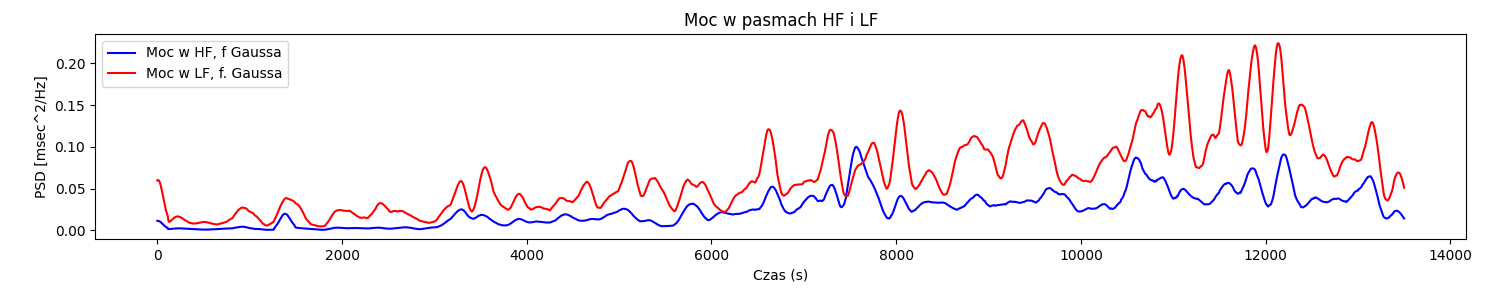
\includegraphics[width=\textwidth]{Rysunki/lf_hf_normal.png}
    \caption{Wykres zmian mocy w pasmach LF i HF w czasie, z zastosowaniem �redniej krocz�cej z filtrem Gaussa.}
    \label{fig:lf_hf_normal}
\end{figure}

\FloatBarrier

W przypadku poprawnego zobrazowania zmienno�ci stosunku mocy w pasmach LF/HF mo�liwe jest zastosowanie r�nych podej��. Na wykresie \ref{fig:lf_hf_avg_ratio} pokazano zmiany tego stosunku w czasie


\begin{figure}[ht]
    \centering
    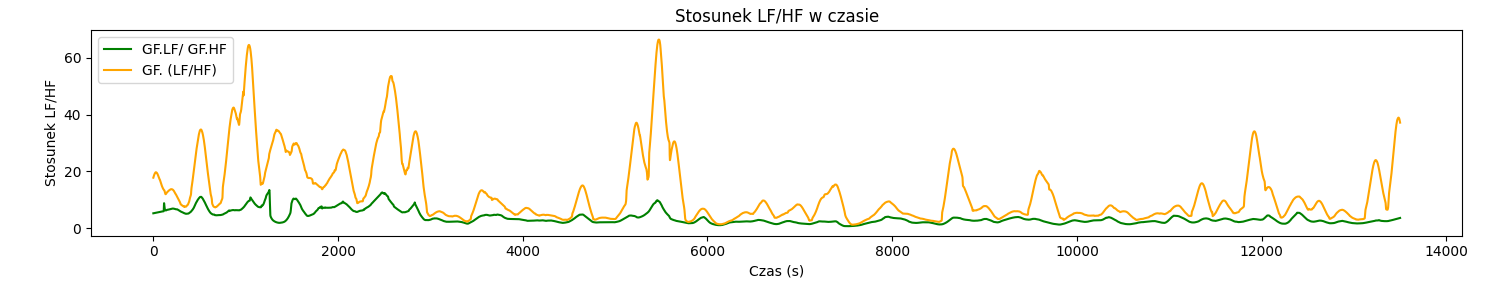
\includegraphics[width=\textwidth]{Rysunki/lf_hf_avg_ratio.png}
    \caption{Por�wnanie dw�ch podej�� do prezentacji stosunku mocy w pasmach LF i HF.}
    \label{fig:lf_hf_avg_ratio}
\end{figure}

\FloatBarrier

gdzie:
\begin{itemize}
    \item Zielon� lini� zilustrowano iloraz warto�ci u�rednionej mocy w pa�mie LF oraz u�rednionej mocy w pa�mie HF dla ka�dego momentu \( t \).
    \item ��t� lini� przedstawiono iloraz rzeczywistej warto�ci mocy w pa�mie LF do warto�ci mocy w pa�mie HF dla chwili \( t \), a nast�pnie wynikow� seri� danych poddano u�rednianiu krocz�cemu.
\end{itemize}

Wida�, �e stosunek tych dw�ch miar jest silniej zale�ny od chwilowych du�ych zmian w warto�ciach w drugim podej�ciu, co utrudnia analiz� trend�w w d�u�szej perspektywie. Dlatego system domy�lnie wykorzystuje pierwsze podej�cie do prezentacji stosunku LF/HF w czasie.

System umo�liwia implementacj� centralnej �redniej krocz�cej wy��cznie dla danych wczytanych w ca�o�ci, np. z pliku CSV. Taka �rednia mo�e by� stosowana jedynie do wykres�w opartych na kompletnych danych, gdzie dla ka�dego analizowanego punktu istnieje odpowiednia liczba pr�bek zar�wno z jego lewej, jak i prawej strony. W przypadku analizy danych w czasie rzeczywistym, gdzie przysz�e warto�ci s� nieznane, tego rodzaju u�rednianie w tej implementacji nie jest wspierane. W takiej sytuacji stosuje si� �rednie oparte wy��cznie na danych historycznych, co powoduje przesuni�cie (tzw. lag) wzgl�dem rzeczywistego sygna�u. W d�u�szym okresie przesuni�cie to ma jednak niewielki wp�yw na og�ln� analiz�.

Funkcjonalno�� obliczania �redniej krocz�cej, zar�wno centralnej, jak i klasycznej, zosta�a r�wnie� zaimplementowana w przypadku wizualizacji trend�w pulsu oraz interwa��w RR, z u�yciem filtra gaussowskiego.



% \section{}
\chapter{Eksperymenty}
���
\section{Por�wnanie zastosowanych metod wykrywania za�amk�w R \small{(autor: Jakub Wojtalewicz)}}\label{sczyty-eksperyment}
\subsection{Wprowadzenie}
Celem niniejszego eksperymentu jest ocena skuteczno�ci zastosowanych w pracy
metod wykrywania za�amk�w R w sygnale EKG w danych pochodz�cych z urz�dzenia
Polar H10. Por�wnania dokonano zar�wno na danych dobrej jako��, o niskim
poziomie zak��ce�, jak i na sygnale mniej czystym, charakteryzuj�cym si�
wi�ksz� nieprzewidywalno�ci�.
\subsection{Definicja miar do analizy wynik�w}
Analiz� wynik�w przeprowadzono na podstawie miar takich jak czu�o�� (recall),
precyzja (precision), oraz ich �rednia harmoniczna, czyli F1. Miary te obliczne
s� na podstawie warto�ci TP (True Positive), FP (False Positive), oraz FN
(False Negative). Spos�b obliczania oraz kr�tki opis wspomnianych metryk
znajduje si� poni�ej:
\begin{itemize}
    \item \textbf{TP (True Positive)} - liczba przypadk�w, w kt�rych model prawid�owo rozpozna� za�amki R
    \item \textbf{FP (False Positive)} - liczba przypadk�w, w kt�rych model b��dnie zaklasyfikowa� fragment sygna�u jako sczyt R
    \item \textbf{FN (False Negative)} - liczba przypadk�w, w kt�rych model nie rozpozna� rzeczywistego za�amka R.
    \item \textbf{Czu�o�� (Recall)} � wskazuje, jaka cz�� rzeczywistych pozytywnych przypadk�w zosta�a poprawnie zidentyfikowana:
          \begin{equation}
              \text{Recall} = \frac{TP}{TP + FN}
          \end{equation}

    \item \textbf{Precyzja (Precision)} � wskazuje, jaka cz�� przewidzianych pozytywnych przypadk�w jest rzeczywi�cie poprawna:
          \begin{equation}
              \text{Precision} = \frac{TP}{TP + FP}
          \end{equation}

    \item \textbf{F1} � �rednia harmoniczna czu�o�ci i precyzji, kt�ra daje zbalansowan� miar� tych dw�ch wska�nik�w:
          \begin{equation}
              F1 = 2 \cdot \frac{\text{Precision} \cdot \text{Recall}}{\text{Precision} + \text{Recall}}
          \end{equation}
\end{itemize}

\subsection{Trening modelu}
Przeprowadzono trening dw�ch wariant�w modelu sieci UNet. Pierwszy wariant
wytrenowano na danych pacjent�w ze zbioru MIT-BIH, a drugi na zbiorze MIT-BIH
Noise Stress, kt�ry zawiera dane wybranych pacjent�w z pierwotnego zbioru,
wzbogacone o szum oraz zjawisko dryftu linii izoelektrycznej (baseline wander).
Oba zbiory zawieraj� adnotacje dotycz�ce lokalizacji szczyt�w R. Do treningu i
oceny wydajno�ci sieci UNet zastosowano okna o d�ugo�ci 10 sekund, poniewa� w
trakcie fazy projektowej taki rozmiar wykazywa� najwy�sz� skuteczno��. Modele
by�y trenowane przez 30 epok, przy u�yciu funkcji straty Binary Crossentropy
oraz optymalizatora Adam do dostosowywania wag modelu.

Po wytrenowaniu modeli przeprowadzono ich ewaluacj� na tych samych zbiorach
danych, na kt�rych by�y trenowane, por�wnuj�c wyniki klasyfikacji z
oznaczeniami wykonanymi przez specjalist�w. Wst�pne rezultaty przedstawiono w
tabeli \ref{wyniki1}.
\begin{table}[ht]
    \captionsetup{justification=centering}
    \caption{Wyniki pierwszego testu modeli na zbiorach treningowych}
    \centering
    \begin{tabular}{|l|c|c|}
        \hline
        \multicolumn{1}{|l|}{} & \multicolumn{1}{l|}{\textbf{MIT-BIH}} & \multicolumn{1}{c|}{\textbf{MIT-BIH Noise Stress}} \\
        \hline
        TP                     & $33436$                               & $5801$                                             \\
        \hline
        FP                     & $76273$                               & $19992$                                            \\
        \hline
        FN                     & $79211$                               & $20569$                                            \\
        \hline
        Recall                 & $0,297$                               & $0,220$                                            \\
        \hline
        Precision              & $0,305$                               & $0,225$                                            \\
        \hline
        F1                     & $0,301$                               & $0,222$                                            \\
        \hline
    \end{tabular}
    \label{wyniki1}
\end{table}
Otrzymane wyniki by�y zaskakuj�ce, co sk�oni�o do dok�adniejszej analizy przyczyn b��d�w w
postaci graficznej. Inspekcja wizualna ujawni�a przesuni�cie wielu etykiet
wzgl�dem rzeczywistych maksim�w sygna�u, co by�o trudne do wyja�nienia.
Przyk�ad tego zjawiska zaprezentowano na Rys. \ref{fig/zleEtykietyMit}. Na wykresie ��te znaczniki reprezentuj� pozycje szczyt�w wed�ug etykiet, niebieskie wskazuj� miejsca, gdzie model rozpozna� szczyty, natomiast czerwone oznaczaj� punkty, w kt�rych etykiety pokrywaj� si� z detekcjami dokonanymi przez model

\begin{figure}[ht]
    \centering
    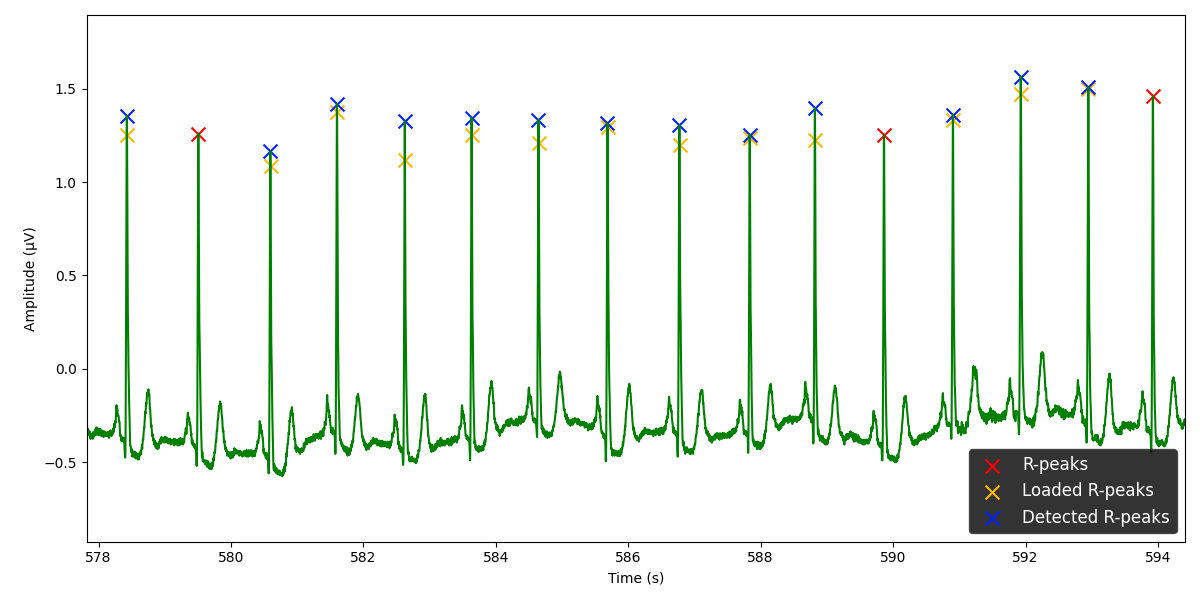
\includegraphics[width=\textwidth]{Rysunki/nieprecyzyjne etykiety.png}
    \caption{Przyk�ad nieprecyzyjnych etykiet w zbiorze MIT-BIH.}
    \label{fig/zleEtykietyMit}
\end{figure}

W wielu przypadkach etykiety by�y nieznacznie przesuni�te wzgl�dem
rzeczywistego szczytu, cz�sto o kilka pr�bek, podczas gdy szczyty przewidywane
przez sie� charakteryzowa�y si� wi�ksz� precyzj�. Aby umo�liwi� bardziej
adekwatn� analiz� wynik�w, uwzgl�dniaj�c� rzeczywist� jako�� przewidywa�,
wprowadzono tolerancj� wynosz�c� 30 ms. Rozpoznanie szczytu w odleg�o�ci do 30
ms od etykiety uznano za prawdziwie pozytywne (TP). Wyniki po zastosowaniu
tolerancji przedstawiono w tabeli \ref{wyniki2}, a tak�e graficznie na Rys.
\ref{fig/poprawioneEtykietyMit}, gdzie bia�y kolor znacznika oznacza punkty
wykryte w granicach przyj�tej tolerancji.

\begin{table}[ht]
    \captionsetup{justification=centering}
    \caption{Wyniki drugiego testu modeli na zbiorach treningowych - po wprowadzeniu tolerancji}
    \centering
    \begin{tabular}{|l|c|c|}
        \hline
        \multicolumn{1}{|l|}{} & \multicolumn{1}{l|}{\textbf{MIT-BIH}} & \multicolumn{1}{c|}{\textbf{MIT-BIH Noise Stress}} \\
        \hline
        TP                     & $105183$                              & $24341$                                            \\
        \hline
        FP                     & $4526$                                & $1453$                                             \\
        \hline
        FN                     & $7464$                                & $2029$                                             \\
        \hline
        Recall                 & $0,934$                               & $0,923$                                            \\
        \hline
        Precision              & $0,959$                               & $0,944$                                            \\
        \hline
        F1                     & $0,946$                               & $0,933$                                            \\
        \hline
    \end{tabular}
    \label{wyniki2}
\end{table}
\begin{figure}[ht]
    \centering
    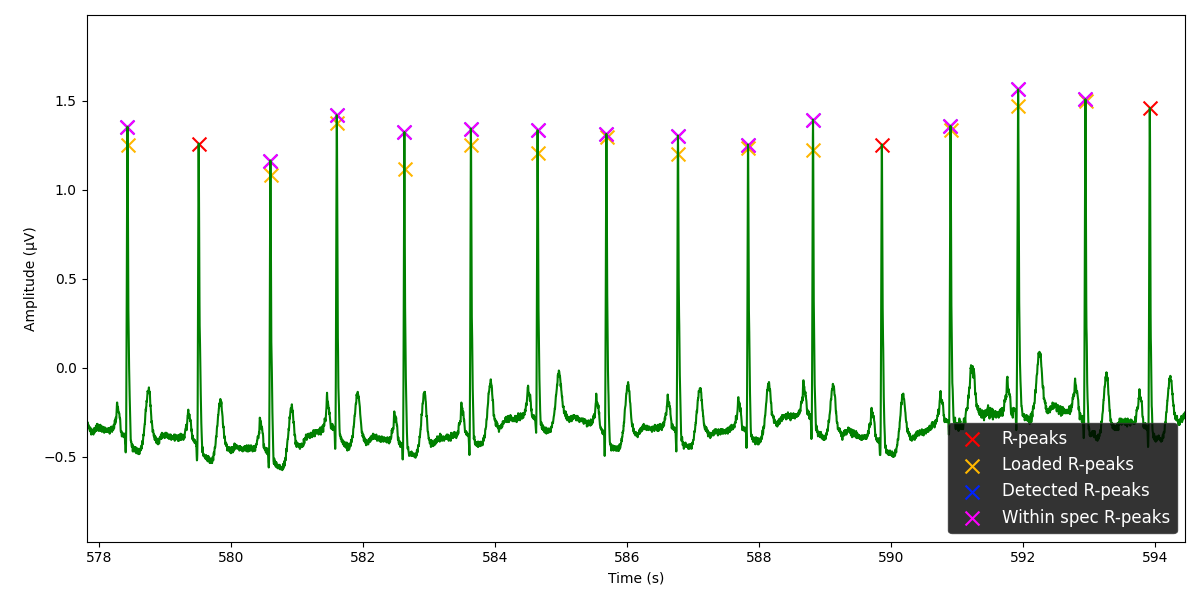
\includegraphics[scale=0.5]{Rysunki/etykiety z tolerancja.png}
    \caption{Wyniki klasyfikacji po wprowadzeniu tolerancji}
    \label{fig/poprawioneEtykietyMit}
\end{figure}

\subsection{Zastosowanie modeli na danych z Polar H10}
Dane w zbiorach MIT-BIH zosta�y zarejestrowane z cz�stotliwo�ci� pr�bkowania
360 Hz, natomiast dane z czujnika Polar H10 s� zbierane z cz�sto�ci� 130 Hz.
Aby umo�liwi� wykorzystanie modeli wytrenowanych na danych o innej
cz�stotliwo�ci pr�bkowania ni� dane testowe, mo�na zastosowa� jedno z dw�ch
podej��. Pierwsze polega na redukcji cz�stotliwo�ci wy�szego pr�bkowania do
ni�szego poprzez decymacj�, co wi��e si� z utrat� cz�ci szczeg�owo�ci danych.
Drugie podej�cie zak�ada zwi�kszenie cz�stotliwo�ci pr�bkowania zbioru o
ni�szej cz�stotliwo�ci, na przyk�ad poprzez interpolacj�. W niniejszym
eksperymencie zastosowano drugie podej�cie � dane z czujnika Polar H10 poddano
interpolacji liniowej do 360 Hz, z wykorzystaniem funkcji \emph{interp1d} z
modu�u \emph{scipy.interpolate}.

\subsection{Analiza danych wysokiej jako�ci}
W trakcie analizy danych pozbawionych zak��ce� przeprowadzono empiryczn� ocen�
algorytmu Pan-Tompkinsa, kt�ry wykaza� si� bardzo wysok� skuteczno�ci�. W
analizowaym 24-godzinnym fragmencie danych zaobserwowano jedynie sporadyczne
przypadki fa�szywie negatywne (FN), co przek�ada sie na ponad 99\% trafnych
klasyfikacji. Z tego wzgl�du algorytm Pan-Tompkinsa zosta� uznany za �z�oty
standard� w tym przypadku, wzgl�dem kt�rego oceniono wydajno�� modeli UNet.
Wyniki por�wnania modeli z wynikami algorytmu Pan-Tompkinsa dla 24 godzinnej
pr�bki z urz�dzenia Polar H10 przedstawiono w tabeli \ref{wynikiClearUnet}. Na
podstawie przeprowadzonej analizy stwierdzono, �e oba algorytmy bardzo dobrze
radz� sobie z sygna�em wysokiej jako�ci.

\begin{table}[ht]
    \captionsetup{justification=centering}
    \caption{Wyniki klasyfikacji wariant�w sieci UNet wzgl�dem warto�ci wyznaczonych przez algorytm Pan-Tompkins dla 24 godzinnego odcinka danych}
    \centering
    \begin{tabular}{|l|c|c|}
        \hline
        \multicolumn{1}{|l|}{} & \multicolumn{1}{l|}{\textbf{MIT-BIH}} & \multicolumn{1}{c|}{\textbf{MIT-BIH Noise Stress}} \\
        \hline
        TP                     & $93903$                               & $93899$                                            \\
        \hline
        FP                     & $16$                                  & $95$                                               \\
        \hline
        FN                     & $83$                                  & $87$                                               \\
        \hline
        Recall                 & $>0.999$                              & $0,999$                                            \\
        \hline
        Precision              & $>0.999$                              & $0,999$                                            \\
        \hline
        F1                     & $>0.999$                              & $0,999$                                            \\
        \hline
    \end{tabular}
    \label{wynikiClearUnet}
\end{table}

\subsection{Analiza danych zaszumionych}
% W przypadku danych zaszumionych empiryczna ocena wykaza�a liczne nieprawid�owo�ci w dzia�aniu algorytmu Pan-Tompkinsa. Przyk�ad b��dnego dzia�ania algorytmu przedstawiono na Rys. ref{rys1}. Z tego powodu, w celu okre�lenia skuteczno�ci algorytm�w przeprowadzono r�czne etykietowanie fragmentu danych z czujnika Polar H10. Nale�y jednak zaznaczy�, �e etykietyzacja nie zosta�a przeprowadzono przez specjalist�, z potwierdzon� wiedz� medyczn�, a przez autor�w niniejszej pracy, tzn. student�w kierunku informatycznego, co mog�o wp�yn�c na jako�� etykiet.

W przypadku danych zaszumionych manualna ocena wykaza�a liczne
nieprawid�owo�ci w dzia�aniu algorytmu Pan-Tompkinsa. Problemy te wynika�y
g��wnie z obecno�ci zak��ce�, takich jak szum czy dryft linii izoelektrycznej
(baseline wander), kt�re znacz�co utrudnia�y prawid�owe wykrywanie za�amk�w R.
Przyk�ad b��dnego dzia�ania algorytmu przedstawiono na Rys.
\ref{fig/zaszumionyTompkins}, gdzie zauwa�alne jest pomijanie istotnych
szczyt�w sygna�u.

\begin{figure}[ht]
    \centering
    % 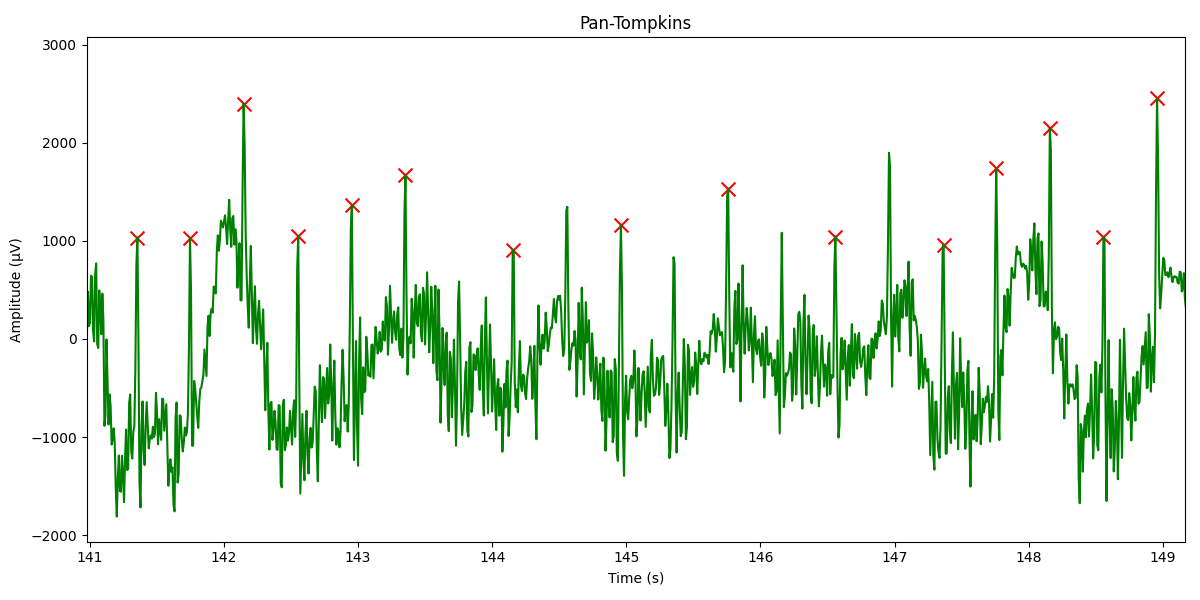
\includegraphics[scale=0.5]{Rysunki/faultyPanTompkins.png}
    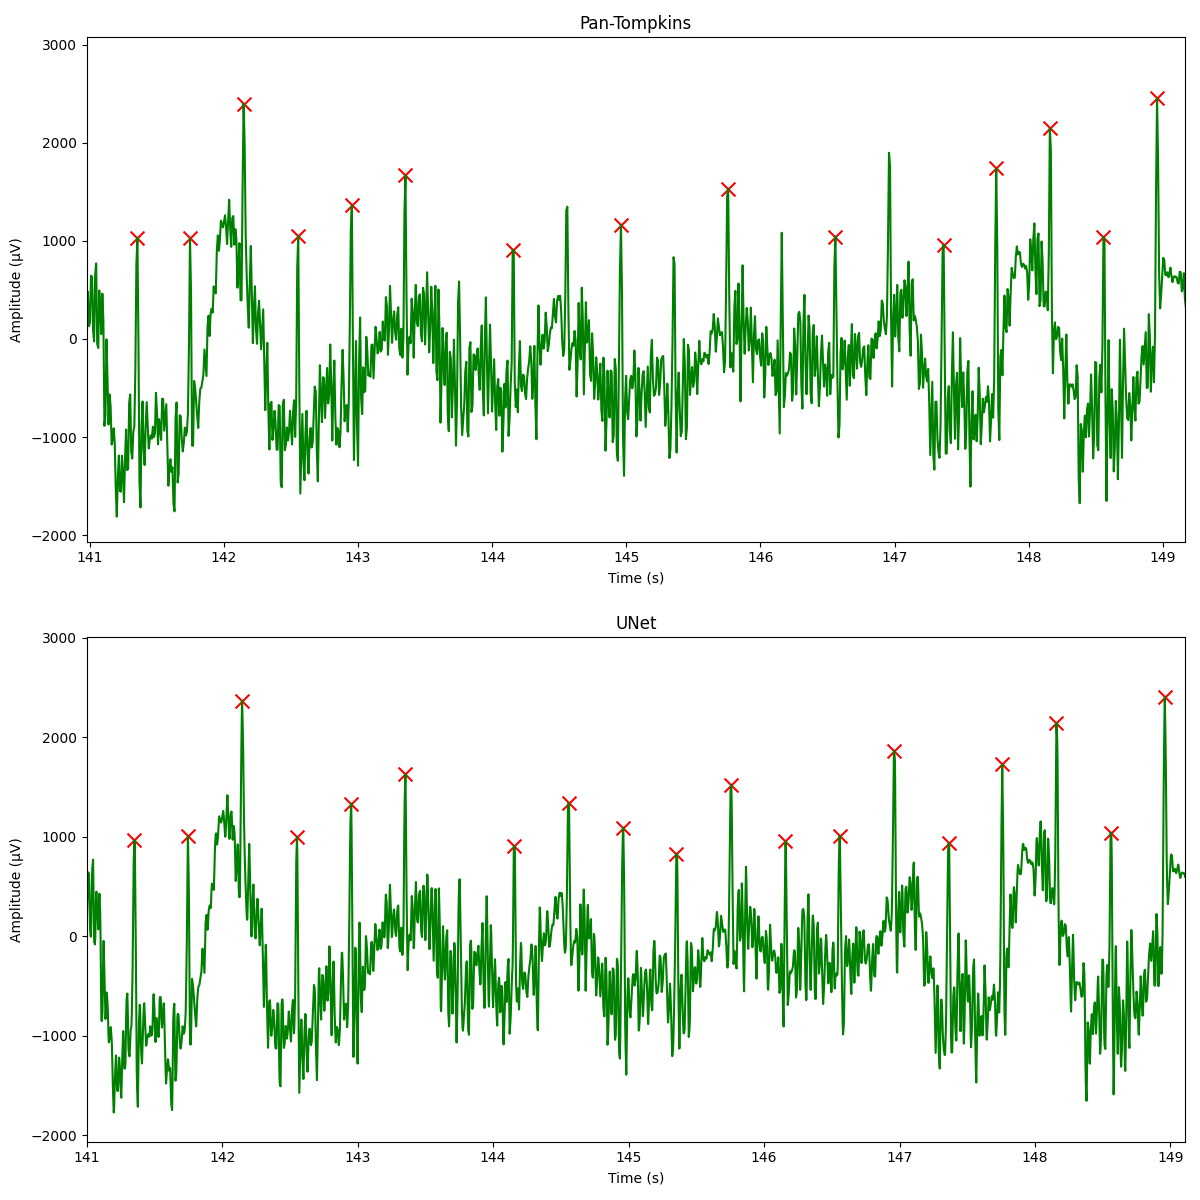
\includegraphics[width=\textwidth]{Rysunki/pt_unet_comparison.png}
    % \caption{Fragment zaszumionego sygna�u EKG, na kt�rym Algorytm Pan-Tompkins nie wykry� wszystkich szczyt�w R}
    \caption{Por�wnanie wykrywania szczyt�w R na przyk�adzie zaszumionego fragmentu sygna�u EKG, z zastosowaniem algorytmu Pan-Tompkinsa oraz wariantu sieci UNet.}
    \label{fig/zaszumionyTompkins}
\end{figure}

W celu przeprowadzenia oceny skuteczno�ci zastosowanych podej��, dokonano
r�cznego oznaczenia fragmentu danych pochodz�cego z czujnika Polar H10. Nale�y
zaznaczy�, �e etykietyzacja nie zosta�a przeprowadzona przez specjalist�, z
potwierdzon� wiedz� medyczn�, a przez autor�w niniejszej pracy, co mog�o
wp�yn�c na jako�� samych etykiet.

Wyniki dzia�ania poszczeg�lnych algorytm�w uzyskane na oznaczonym fragmencie
danych przedstawiono w tabeli \ref{wynikiClearUnet}. Analizuj�c jej zawarto��
mo�na doj�� do wniosku, �e warianty sieci UNet lepiej radz� sobie z
klasyfikacj� sygna��w zaszumionych w por�wnaniu do algorytmu Pan-Tompkinsa.
Modele UNet wykaza�y du�o wi�ksz� ilo�ci� szczyt�w poprawnie zaklasyfikowanych
(TP), mniejsz� liczb� pomini�tych za�amk�w (FN) oraz, w przypadku wariantu
trenowanego na zbiorze zaszumionym, ni�sz� liczb� fa�szywych trafie� (FP).

Uzyskane rezultaty sugeruj� przewag� modeli UNet nad zastosowanym algorytmem
Pan-Tompkinsa w przypadku zaszumionych sygna��w. Na cele tego eksperymentu
zdecydowano si� na ocen� sygna�u zawieraj�cego oko�o 300 szczyt�w, niemniej
jednak, aby uzyka� bardziej kompleksow� ocen� skuteczno�ci zastosowanych metod,
nale�a�oby zebra� oraz r�cznie oznaczy� znacznie wi�ksz� pr�b� danych.

\begin{table}[ht]
    \captionsetup{justification=centering}
    \caption{Wyniki wariant�w sieci UNet oraz algorytmu Pan-Tompkins wzgl�dem r�cznie wyznaczonych etykiet na fragmencie sygna�u}
    \centering
    \begin{tabular}{|l|c|c|c|}
        \hline
        \multicolumn{1}{|l|}{} & \multicolumn{1}{l|}{\textbf{Pan-Tompkins}} & \multicolumn{1}{l|}{\textbf{MIT-BIH}} & \multicolumn{1}{c|}{\textbf{MIT-BIH Noise Stress}} \\
        \hline
        TP                     & $212$                                        & $272$                                   & 276                                                \\
        \hline
        FP                     & $4$                                          & $5$                                     & 2                                                  \\
        \hline
        FN                     & $77$                                         & $17$                                    & 13                                                 \\
        \hline
        Recall                 & $0.734$                                      & $0,941$                                 & 0,955                                              \\
        \hline
        Precision              & $0.981$                                      & $0,982$                                 & 0,993                                              \\
        \hline
        F1                     & $0.840$                                      & $0,961$                                 & 0,974                                              \\
        \hline
    \end{tabular}
    \label{wynikiClearUnet}
\end{table}

\subsection{Wnioski}
Zastosowane warianty sieci UNet oraz algorytm Pan-Tompkinsa uzyska�y �wietn�
skuteczno�� w rozpoznawaniu szczyt�w R w sygna�ach dobrej jako�ci, wykazuj�c
marginalne r�nice miedzy dokonywanymi klasyfikacjami. Wi�ksze odchy�y w
wynikach zauwa�ono podczas analizy sygna��w mniej idealnych, gdzie lepsze
rezultaty uzyska�y oba przetronowane modele sieci neuronowych.

W praktycznych zastosowaniach niemal niemo�liwe jest uzyskanie sygna�u
ca�kowicie pozbawionego szum�w. Na podstawie tej obserwacji oraz uzyskanych
wynik�w mo�na stwierdzi�, �e w przypadku analizy sygna�u EKG pochodz�cego z
czujnika Polar H10 lepszym wyborem jest zastosowanie modelu UNet
przetrenowanego na zaszumionym zbiorze danych. Model ten wykaza� por�wnywaln�
dok�adno�� z innymi metodami w przypadku sygna��w wysokiej jako�ci, a
jednocze�nie znacznie lepsz� skuteczno�� w analizie sygna��w o ni�szej jako�ci.



\section{Przewidywanie parametr�w HRV oraz RSA przy u�yciu sieci neuronowej opartej na interwa�ach RR}\label{RRsiec}

\subsection{Wprowadzenie}
Jako etap po�redni w tworzeniu sieci end-to-end do przewidywania miar HRV i RSA
na podstawie sygna�u z Polara H10 opracowano model, kt�ry przewiduje te miary
na podstawie interwa��w RR. Docelowym zamiarem by�o zintegrowanie tego modelu z
sieci� UNet w jeden kompleksowy system end-to-end. Pr�by stworzenia takiej
sieci jednak nie przynios�y oczekiwanych rezultat�w. Za przyczyn� uznano
z�o�ono�� procesu przetwarzania wynik�w wymaganego przez sie� UNet, kt�rego
implementacji jako wewn�trznej warstwy modelu nie uda�o si� zrealizowa�.

Niniejszy eksperyment stanowi wi�c jedynie �proof of concept� - analizuje on
wyniki dw�ch roz��cznych sieci dzia�aj�cych razem. Stanowi r�wnie� punkt
odniesienia dla modelu end-to-end, omawianego w ramach nast�pnego eksperymentu.

\subsection{Definicja miar oceny modeli}
Do analizy uzyskanych wynik�w zastosowano nast�puj�ce miary:

\begin{itemize}
    \item �redni b��d bezwzgl�dny (Mean Absolute Error, MAE): �rednia arytmetyczna warto�ci bezwzgl�dnych r�nic mi�dzy warto�ciami rzeczywistymi a przewidywanymi.
          \begin{equation}
              \text{MAE} = \frac{1}{n} \sum_{i=1}^n |y_i - \hat{y}_i|
          \end{equation}

    \item B��d �redniokwadratowy (Mean Squared Error, MSE): �rednia arytmetyczna
          kwadrat�w r�nic mi�dzy warto�ciami rzeczywistymi a przewidywanymi,
          podkre�laj�ca wi�ksze b��dy.
          \begin{equation}
              \text{MSE} = \frac{1}{n} \sum_{i=1}^n (y_i - \hat{y}_i)^2
          \end{equation}

    \item Pierwiastek ze �redniego b��du kwadratowego (Root Mean Squared Error, RMSE):
          Pierwiastek kwadratowy z MSE, interpretowany w tych samych jednostkach, co dane
          wej�ciowe.
          \begin{equation}
              \text{RMSE} = \sqrt{\frac{1}{n} \sum_{i=1}^n (y_i - \hat{y}_i)^2}
          \end{equation}

    \item Wsp�czynnik determinacji ($R^2$): Miara jako�ci dopasowania modelu do danych.
          Reprezentuje jaka cz�� zmienno��i warto�ci w danych jest wyja�niana przez
          model. Warto�� $R^2$ przyjmuje warto�ci z zakresu od $-\infty$ do 1, gdzie 1
          oznacza idealne dopasowanie, a warto�ci poni�ej 0 �wiadcz�, �e lepiej
          poradzi�aby sobie zwyk�a �rednia.

          \begin{equation}
              R^2 = 1 - \frac{\sum_{i=1}^{n} (y_i - \hat{y}_i)^2}{\sum_{i=1}^{n} (y_i - \bar{y})^2}
          \end{equation}
          gdzie:
          \begin{itemize}
              \item \( n \) � liczba analizowanych warto�ci,
              \item \( y_i \) � warto�� rzeczywista dla i-tej obserwacji,
              \item \( \hat{y}_i \) � warto�� przewidywana przez model dla i-tej obserwacji,
              \item \( \bar{y} \) � �rednia warto�� rzeczywistych obserwacji.
          \end{itemize}
\end{itemize}

\subsection{Metodologia}
W ramach tego eksperymentu obie sieci funkcjonuj� w uk�adzie kaskadowym. W
pierwszym etapie wariant sieci UNet, wytrenowany na zaszumionym zbiorze danych
(kt�rego skuteczno�� by�a oceniana w poprzednim eksperymencie), wykrywa szczyty
R w sygnale EKG. Na podstawie tych detekcji obliczane s� interwa�y RR, kt�re
nast�pnie dzielone s� na okna czasowe. Te okna stanowi� wej�cie do drugiej
sieci, odpowiedzialnej za obliczanie miar HRV i RSA. D�ugo�� ka�dego okna
ustalono na 300 pr�bek interwa��w RR, co odpowiada oko�o 5 minutom pracy serca
przy �rednim pulsie wynosz�cym 60 uderze� na minut�. Jako�� przewidywa�
drugiego modelu by�a oceniana wzgl�dem metryk wyliczonych w spos�b tradycyjny,
podstawiaj�c warto�ci do wzor�w przedstawionych w podrozdziale \ref{MiaryHRV}.
Do oblicze� wykorzystano r�wnie� szczyty R zidentyfikowane przez sie� UNet.

\subsection{Warianty modeli oraz ich trening}
W ramach eksperymentu rozwa�ano r�ne konfiguracje i zakresy miar HRV oraz RSA
przewidywanych przez sie�. Analizowane warianty obejmowa�y mi�dzy innymi:
przewidywanie wy��cznie SDNN, wy��cznie RMSSD, jednoczesne przewidywanie SDNN i
RMSSD, a tak�e przewidywanie znormalizowanych miar LF i HF.

Do ewaluacji modelu wykorzystano zbi�r w�asny, zawieraj�cy sumarycznie ok. 48h
zapisu sygna�u EKG oraz metod� 5-krotnej walidacji krzy�owej, s�u��cej
wiarygodnej ocenie jako�ci przewidywa�

\subsection{Wyniki}
�rednie wyniki uzyskane w ramach walidacji krzy�owej dla wybranych modeli przedstawiono w tabelach \ref{wyniki_hrv_pojedyncze_rr}, \ref{wyniki_hrv_wiele_rr} oraz \ref{wyniki_hrv_wiele_rr2}.
\begin{table}[ht]
    \captionsetup{justification=centering}
    \caption{�rednie wyniki walidacji krzy�owej dla modeli przewiduj�cych pojedyncze miary.}
    \centering
    \begin{tabular}{|l|c|c|c|c|c|c|}
        \hline
        \textbf{Wariant} & \textbf{SDNN}     & \textbf{RMSSD}    \\ \hline
        MAE              & $6,02 \pm 0,38$   & $6,74 \pm 1,83$   \\ \hline
        MSE              & $65,07 \pm 16,21$ & $96,73 \pm 62,92$ \\ \hline
        RMSE             & $8,01 \pm 0,94$   & $9,32 \pm 3,15$   \\ \hline
        R2               & $0,93 \pm 0,02$   & $0,74 \pm 0,15$   \\ \hline
    \end{tabular}
    \label{wyniki_hrv_pojedyncze_rr}
\end{table}

\begin{table}[ht]
    \captionsetup{justification=centering}
    \caption{�rednie wyniki walidacji krzy�owej dla modeli przewiduj�cych wiele miar.}
    \centering
    \begin{tabular}{|l|c|c|c|c|c|c|}
        \hline
        \textbf{Wariant} & \multicolumn{2}{|c|}{\textbf{SDNN i RMSSD}} & \multicolumn{2}{|c|}{\textbf{LF norm i HF norm}}                                       \\ \hline
        \textbf{Miara}   & \textbf{SDNN}                               & \textbf{RMSSD}                                   & \textbf{LF norm} & \textbf{HF norm} \\ \hline
        MAE              & $7,43 \pm 1,38$                             & $5,09 \pm 1,55$                                  & $\sim0,06$       & $\sim0,06$       \\ \hline
        MSE              & $92,12 \pm 31,91$                           & $63,32 \pm 62,83$                                & $\sim0,01$       & $\sim0,01$       \\ \hline
        RMSE             & $9,46 \pm 1,65$                             & $7,22 \pm 3,35$                                  & $0,08 \pm 0,01$  & $0,08 \pm 0,01$  \\ \hline
        R2               & $0,91 \pm 0,03$                             & $0,84 \pm 0,12$                                  & $0,52 \pm 0,10$  & $0,52 \pm 0,10$  \\ \hline
    \end{tabular}
    \label{wyniki_hrv_wiele_rr}
\end{table}

\begin{table}[ht]
    \captionsetup{justification=centering}
    \caption{�rednie wyniki walidacji krzy�owej dla modeli przewiduj�cych wiele miar.}
    \centering
    \begin{tabular}{|l|c|c|c|c|c|c|}
        \hline
        \textbf{Wariant} & \multicolumn{4}{|c|}{\textbf{SDNN, RMSSD, LF, HF}}                                                                       \\ \hline
        \textbf{Miara}   & \textbf{SDNN}                                      & \textbf{RMSSD}    & \textbf{LF}             & \textbf{HF}           \\ \hline
        MAE              & $15,01 \pm 2,22$                                   & $6,85 \pm 0,99$   & $159,79 \pm 22.47$      & $63,08 \pm 5,95$      \\ \hline
        MSE              & $407,33 \pm 115,64$                                & $89,15 \pm 46,72$ & $60515,62 \pm 24793,08$ & $8725,61 \pm 1682,30$ \\ \hline
        RMSE             & $19,99 \pm 2,80$                                   & $9,19 \pm 2,18$   & $240,89 \pm 49,86$      & $92,96 \pm 9,16$      \\ \hline
        R2               & $0,60 \pm 0,08$                                    & $0,76 \pm 0,10$   & $0,78 \pm 0,08$         & $0,68 \pm 0,05$       \\ \hline
    \end{tabular}
    \label{wyniki_hrv_wiele_rr2}
\end{table}

Spo�r�d modeli przewiduj�cych pojedyncze miary najlepsze wyniki uzyskano dla
SDNN ($R^2 = 0,93 \pm 0,02$), co wskazuje na wysokie pokrycie z
rzeczywisto�cia. RMSSD uzyska�o ni�sze lecz dalej wysokie $R^2 = 0,74 \pm
    0,15$. R�nica mi�dzy dopasowaniem tych metryk, mo�e wynika� z wy�szej
zmienno��i RMSSD w kr�tszych okresach czasowych. Wariant modelu przewiduj�cy
obie te miary jednocze�nie wykaza� podobnymi lub lepszymi wynikami wzgl�dem
wariant�w z j�dna cech� - dla SDNN uzyskano zblizony wynik dopasowania, a dla
RMSSD lepszy ($R^2 = 0,84 \pm 0,12$). Pomimo dobrego og�lnego dopasowania,
zaobserwowano pogorszenie jako�ci przewidywa� w poszczeg�lnych przypadkach, co
potwierdzaj� wy�sze warto�ci MAE i MSE.

Model przewiduj�cy cztery miary jednocze�nie osi�gn�� mieszane wyniki. Dla
warto�ci LF i RMSSD uzyska� wsp�czynnik determinacji na poziomie oko�o 0,75,
natomiast dla pozosta�ych metryk rezultaty by�y mniej zadowalaj�ce.

\subsection{Wnioski}
Wiele z analizowanych wariant�w modeli wykaza�o dobre dopasowanie do
rzeczywistych warto�ci. Jednak, maj�c na uwadze fakt, �e modele otrzymywa�y na
wej�ciu interwa�y RR, z kt�rych te miary mo�na obliczy� w spos�b bezpo�redni,
uzyskane wyniki nie spe�ni�y w pe�ni oczekiwa�. Gdyby jednak uda�o si�
zintegrowa� przedstawiony model z sieci� UNet w ramach systemu end-to-end,
uzyskane rezultaty mog�yby zosta� uznane za satysfakcjonuj�ce.

\FloatBarrier
\section{Przewidywanie miar HRV oraz RSA za pomoc� sieci typu end-to-end}

\subsection{Wprowadzenie}
Celem niniejszego eksperymentu by�o zbadanie mo�liwo�ci zaprojektowanej sieci
typu end-to-end do przewidywania miar HRV oraz RSA, opisanej szczeg�owo w
podrozdziale \ref{siec-end-to-end}. Przegl�d literatury nie wykaza� istnienia
podobnych rozwi�za� dzia�aj�cych w ten spos�b, co podkre�la innowacyjny
charakter proponowanego podej�cia. Jednocze�nie brak takich rozwi�za�
uniemo�liwia bezpo�rednie por�wnanie wynik�w z innymi badaniami. Eksperyment
mia� na celu ukazanie potencjalnych mo�liwo�ci tego modelu oraz jego
skuteczno�ci w przewidywaniu wybranych miar, na podstawie danych EKG
pochodz�cych z rejestratora Polar H10.

\subsection{Warianty modeli}
W eksperymencie przeanalizowano r�ne warianty zaproponowanej sieci, r�ni�ce
si� ilo�cia oraz rodzajem przewidywanych miar HRV i RSA. Rozwa�ano podobne
konfiguracje jak w przypadku eksperymentu przedstawionego w podrodziale
\ref{RRsiec}. Obejmowa�y one m. in. przewidywanie pojedynczych miar takich jak
SDNN czy RMSSD oraz przewidywanie wielu miar na raz, na przyk�ad jednoczesne
przewidywanie SDNN i RMSSD oraz znormalizowanych warto�ci LF i HF.

\subsection{Przygotowanie danych}
Dane do eksperymentu pochodzi�y z w�asnych nagra� EKG zarejestrowanych za
pomoc� Polar H10, obejmuj�cych ��cznie oko�o 48 godzin. Do treningu i
przewidywa� wykorzystano 5-minutowe fragmenty sygna�u, kt�re wcze�niej
znormalizowano do zakresu od -1 do 1. Warto�ci referencyjne miar by�y obliczane
na podstawie oznacze� za�amk�w R, wytworzonych przez sie� UNet oraz wzor�w
przedstawionych w podrodziale \ref{MiaryHRV}. Wykorzystano wariant sieci
przetrenowany na zaszumionym zbiorze, kt�ry by� przedmiotem szerszej analizy w
poprzednim eksperymencie.

\subsection{Trening oraz metoda ewaluacji skuteczno�ci}
Trening ka�dego modelu przeprowadzono w jednolitych warunkach: przez 150 epok z
u�yciem funkcji straty MSE oraz optymalizatora Adam.

Skuteczno�� ka�dego wariantu sieci oceniono za pomoc� 5-krotnej walidacji
krzy�owej, co zapewni�o wiarygodn� ocen� jako�ci przewidywa� oraz umo�liwi�o
por�wnanie wynik�w mi�dzy r�nymi konfiguracjami modeli.

\subsection{Wyniki}
�rednie wyniki uzyskane w ramach walidacji krzy�owej dla wybranych modeli przedstawiono w tabelach \ref{wyniki_hrv_pojedyncze} oraz \ref{wyniki_hrv_wiele}.

\begin{table}[ht]
    \captionsetup{justification=centering}
    \caption{�rednie wyniki walidacji krzy�owej dla modeli przewiduj�cych pojedyncze miary.}
    \centering
    \begin{tabular}{|l|c|c|c|c|c|c|}
        \hline
        \textbf{Wariant} & \textbf{SDNN}       & \textbf{RMSSD}      \\ \hline
        MAE              & $11,22 \pm 2,15$    & $12,06 \pm 7,26$    \\ \hline
        MSE              & $319,90 \pm 185,50$ & $486,95 \pm 488,95$ \\ \hline
        RMSE             & $17,70 \pm 5,00$    & $19,48 \pm 10,37$   \\ \hline
        R2               & $0,7 \pm 0,17$      & $-0,61 \pm 1,74$    \\ \hline
    \end{tabular}
    \label{wyniki_hrv_pojedyncze}
\end{table}

\begin{table}[ht]
    \captionsetup{justification=centering}
    \caption{�rednie wyniki walidacji krzy�owej dla modeli przewiduj�cych wiele miar.}
    \centering
    \begin{tabular}{|l|c|c|c|c|c|c|}
        \hline
        \textbf{Wariant} & \multicolumn{2}{|c|}{SDNN i RMSSD} & \multicolumn{2}{|c|}{\textbf{LF norm i HF norm}}                                       \\ \hline
        \textbf{Miara}   & \textbf{SDNN}                      & \textbf{RMSSD}                                   & \textbf{LF norm} & \textbf{HF norm} \\ \hline
        MAE              & $9,69 \pm 0,56$                    & $8,32 \pm 1,84$                                  & $0,07 \pm 0,01$  & $0,07 \pm 0,01$  \\ \hline
        MSE              & $191,71 \pm 31,69$                 & $141,93 \pm 49,51$                               & $\sim0,01$       & $\sim0,01$       \\ \hline
        RMSE             & $13,80 \pm 1,17$                   & $11,70 \pm 2,23$                                 & $0,09 \pm 0,01$  & $0,09 \pm 0,01$  \\ \hline
        R2               & $0,81 \pm 0,04$                    & $0,58 \pm 0,13$                                  & $0,42 \pm 0,07$  & $0,42 \pm 0,07$  \\ \hline
    \end{tabular}
    \label{wyniki_hrv_wiele}
\end{table}

Ku zaskoczeniu, najlepsz� jako�� przewidywa� osi�gn�� model jednocze�nie
przewiduj�cy SDNN i RMSSD. Uzyska� on �redni wynik wsp�czynnika $R^2$ na
poziomie ok. 0,8 dla SDNN oraz ok. 0,58 dla RMSSD, co przewy�sza�o rezultaty
uzyskane przez modele przewiduj�ce te miary oddzielnie. Moze to wynika� z
wyst�puj�cej mi�dzy tymi miarami korelacji, kt�ra u�atwia modelowi rozpoznanie
bardziej z�o�onych zale�no�ci. Wyniki tego wariantu dla jednego z fold�w
walidacji krzy�owej przedstawiono na Rys \ref{fig/SDNN_RMSSD}

\begin{figure}[ht]
    \centering
    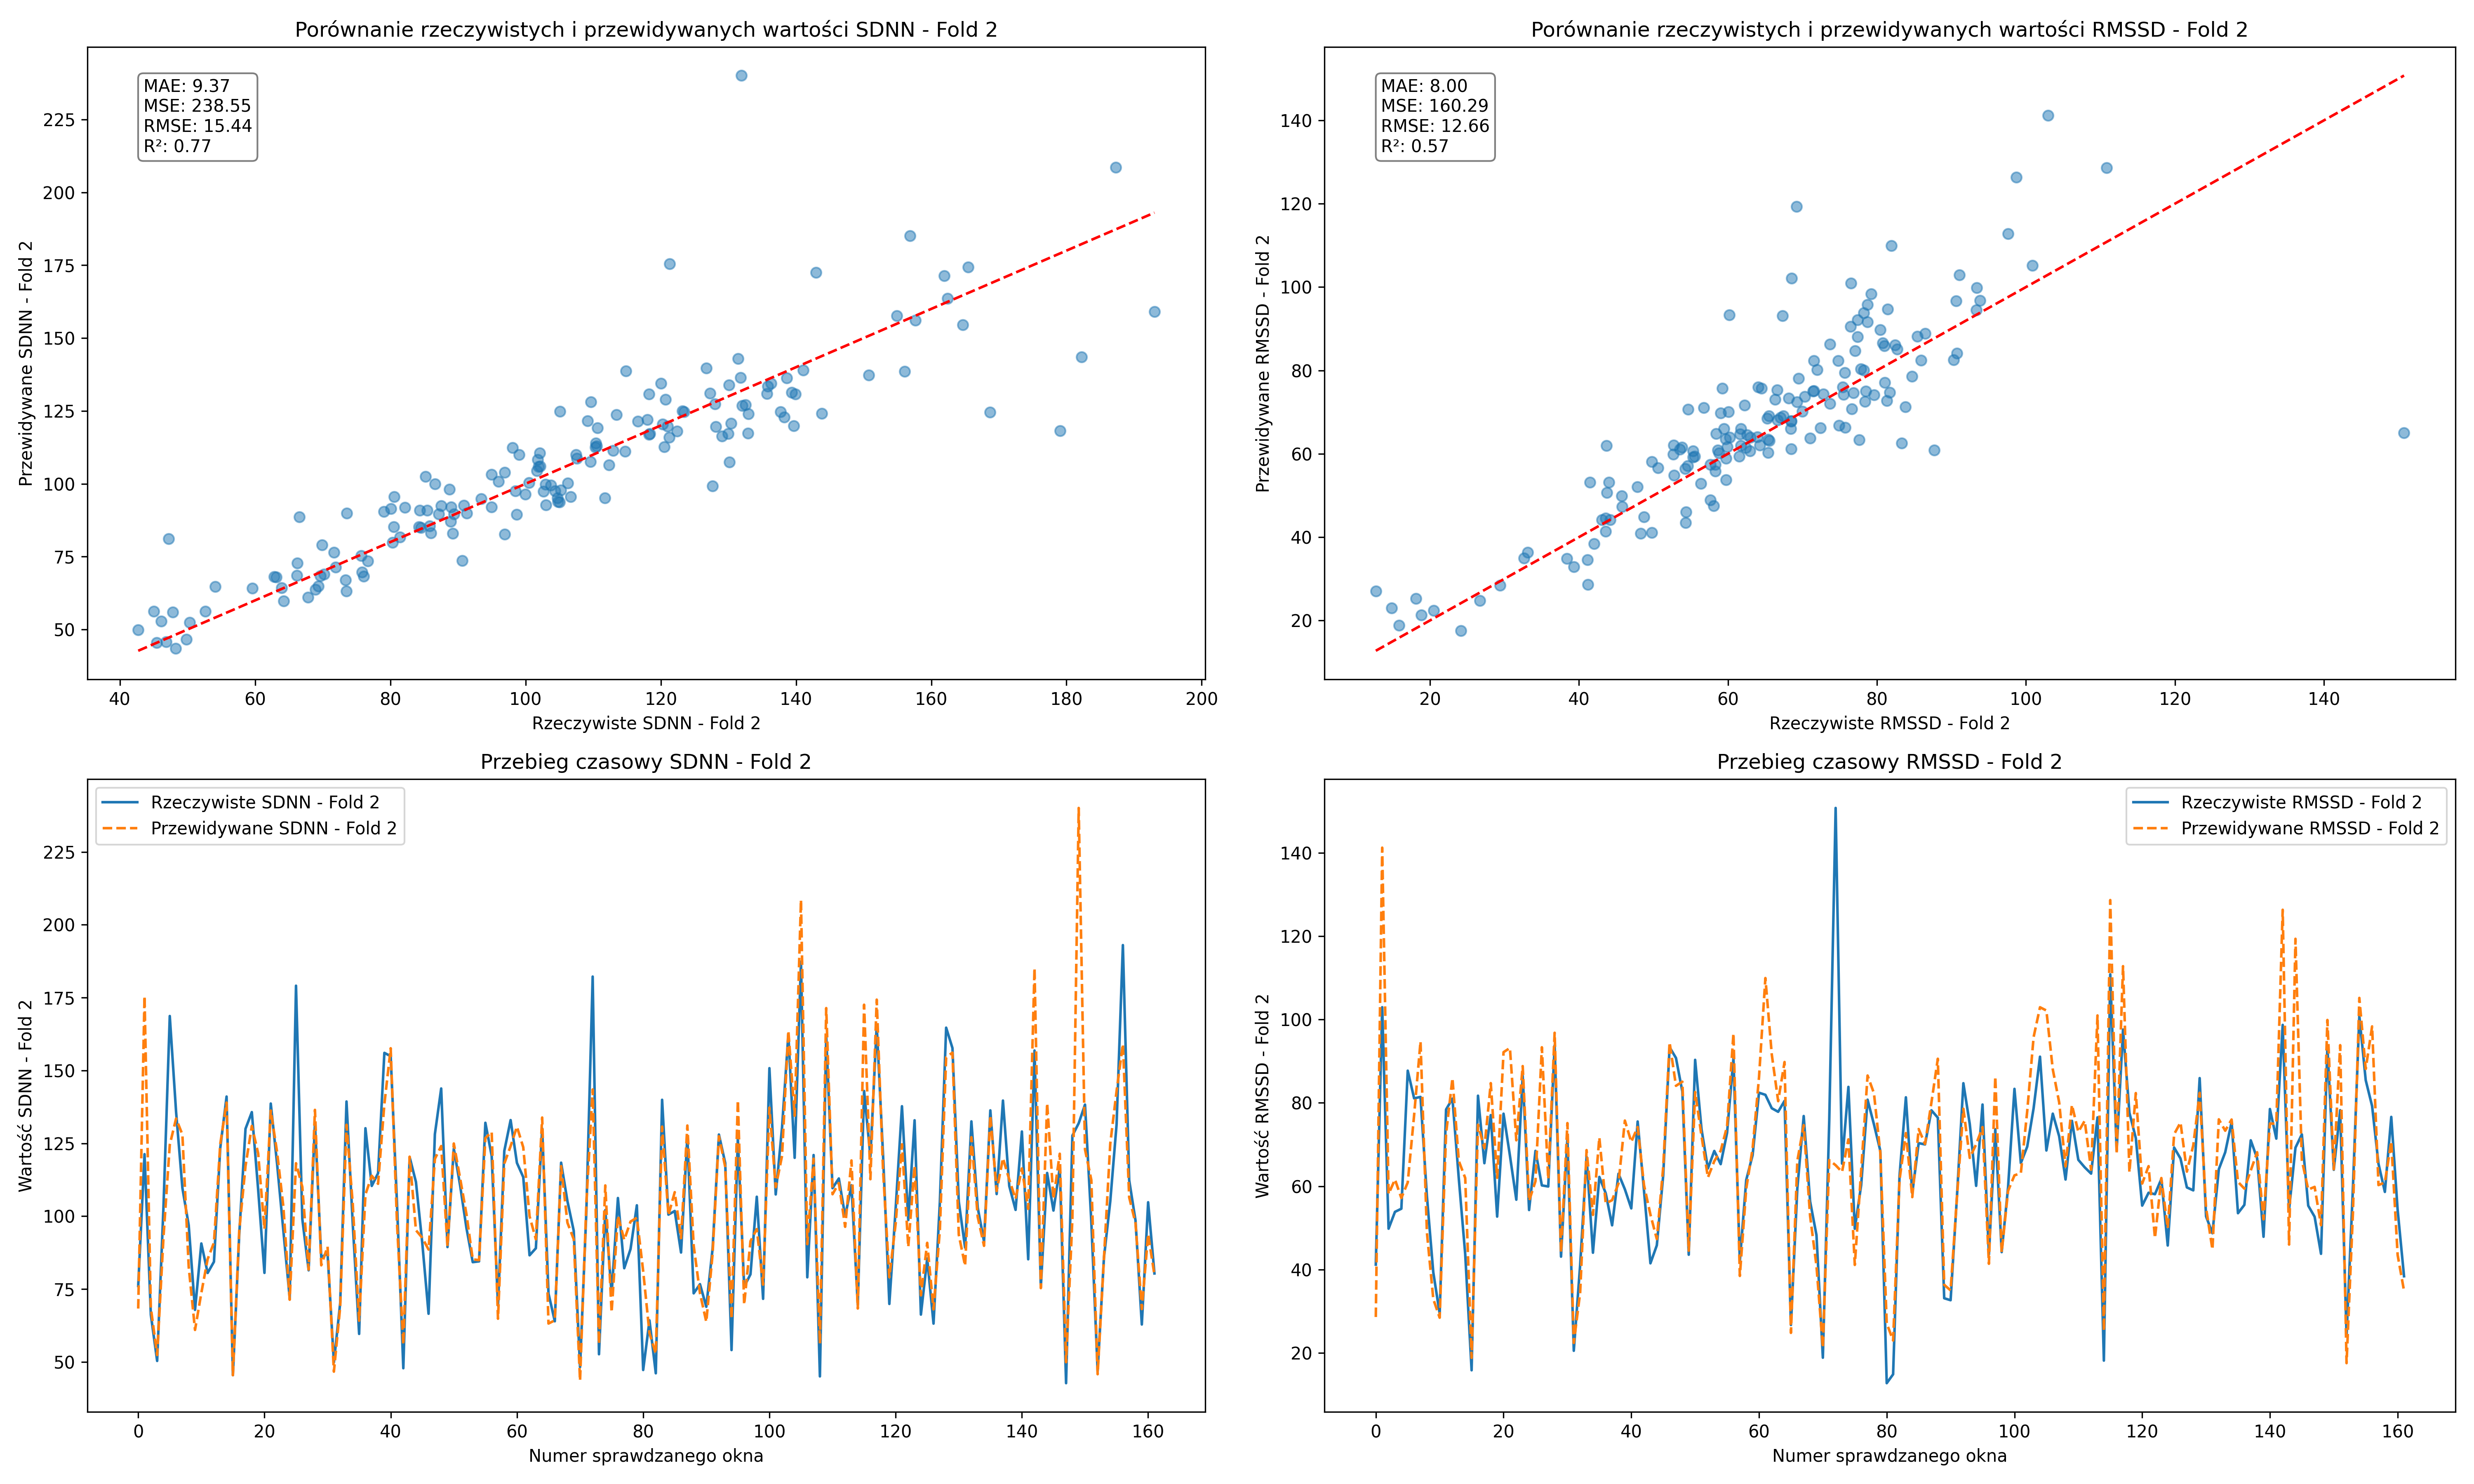
\includegraphics[scale=0.25]{Rysunki/SDNN i RMSSD.png}
    \caption{Wyniki przewidywa� SDNN oraz RMSSD dla jednego z fold�w}
    \label{fig/SDNN_RMSSD}
\end{figure}

Ni�szy wynik wsp�czynnika determinacj RMSSD, wzgl�dem SDNN w tym modelu mo�e
by� zwi�zany z r�nic� w ich typowych warto�ciach. Zastosowana funkcja straty
MSE, faworyzuje redukcj� b��d�w dla miar o wy�szych warto�ciach, co mo�e
prowadzi� do niedoszczacowania warto�ci o mniejszym zakresie.

Wynikiem akceptowalnym wykaza� sie wariant przewiduj�cy jedynie SDNN, kt�ry
uzyska� wsp�czynnik $R^2$ na poziomie $0,7\pm0.17$. Pozosta�e warianty
wykaza�y nisk� zgodno�� przewidywa� z rzeczywisto�ci�, co wskazuje na trudno�ci
modelu w nauce tych miar i ogranicza ich praktyczn� u�yteczno��.

Najwi�kszym zaskoczeniem w trakcie przeprowadzania badania okaza�a sie bardzo
wysoka niesp�jno�� wynik�w mi�dzy foldami w walidacji krzy�owej dla RMSSD. By�a
ona znacznie wi�ksza ni� w przypadku innych sprawdzanych wariant�w. Podczas
analizy fold�w stwierdzono, �e pomimo dobrych rokowa� na niekt�rych zbiorach,
model nie generalizuje si� zbyt dobrze i osi�ga mocno skrajne wyniki w
zale�no�ci od testowanych danych. Przyk�ad ogromnej r�nicy mi�dzy dwoma
foldami przedstawiono na Rys. \ref{fig/RMSSD_2_folds}

W ramach ekperymentu, testowano r�wnie� warianty sieci przewiduj�ce wi�ksz�
liczb� miar ni� dwie, jednak �aden z tych modeli nie osi�gn�� zadowalaj�cych
wynik�w.

\begin{figure}[ht]
    \centering
    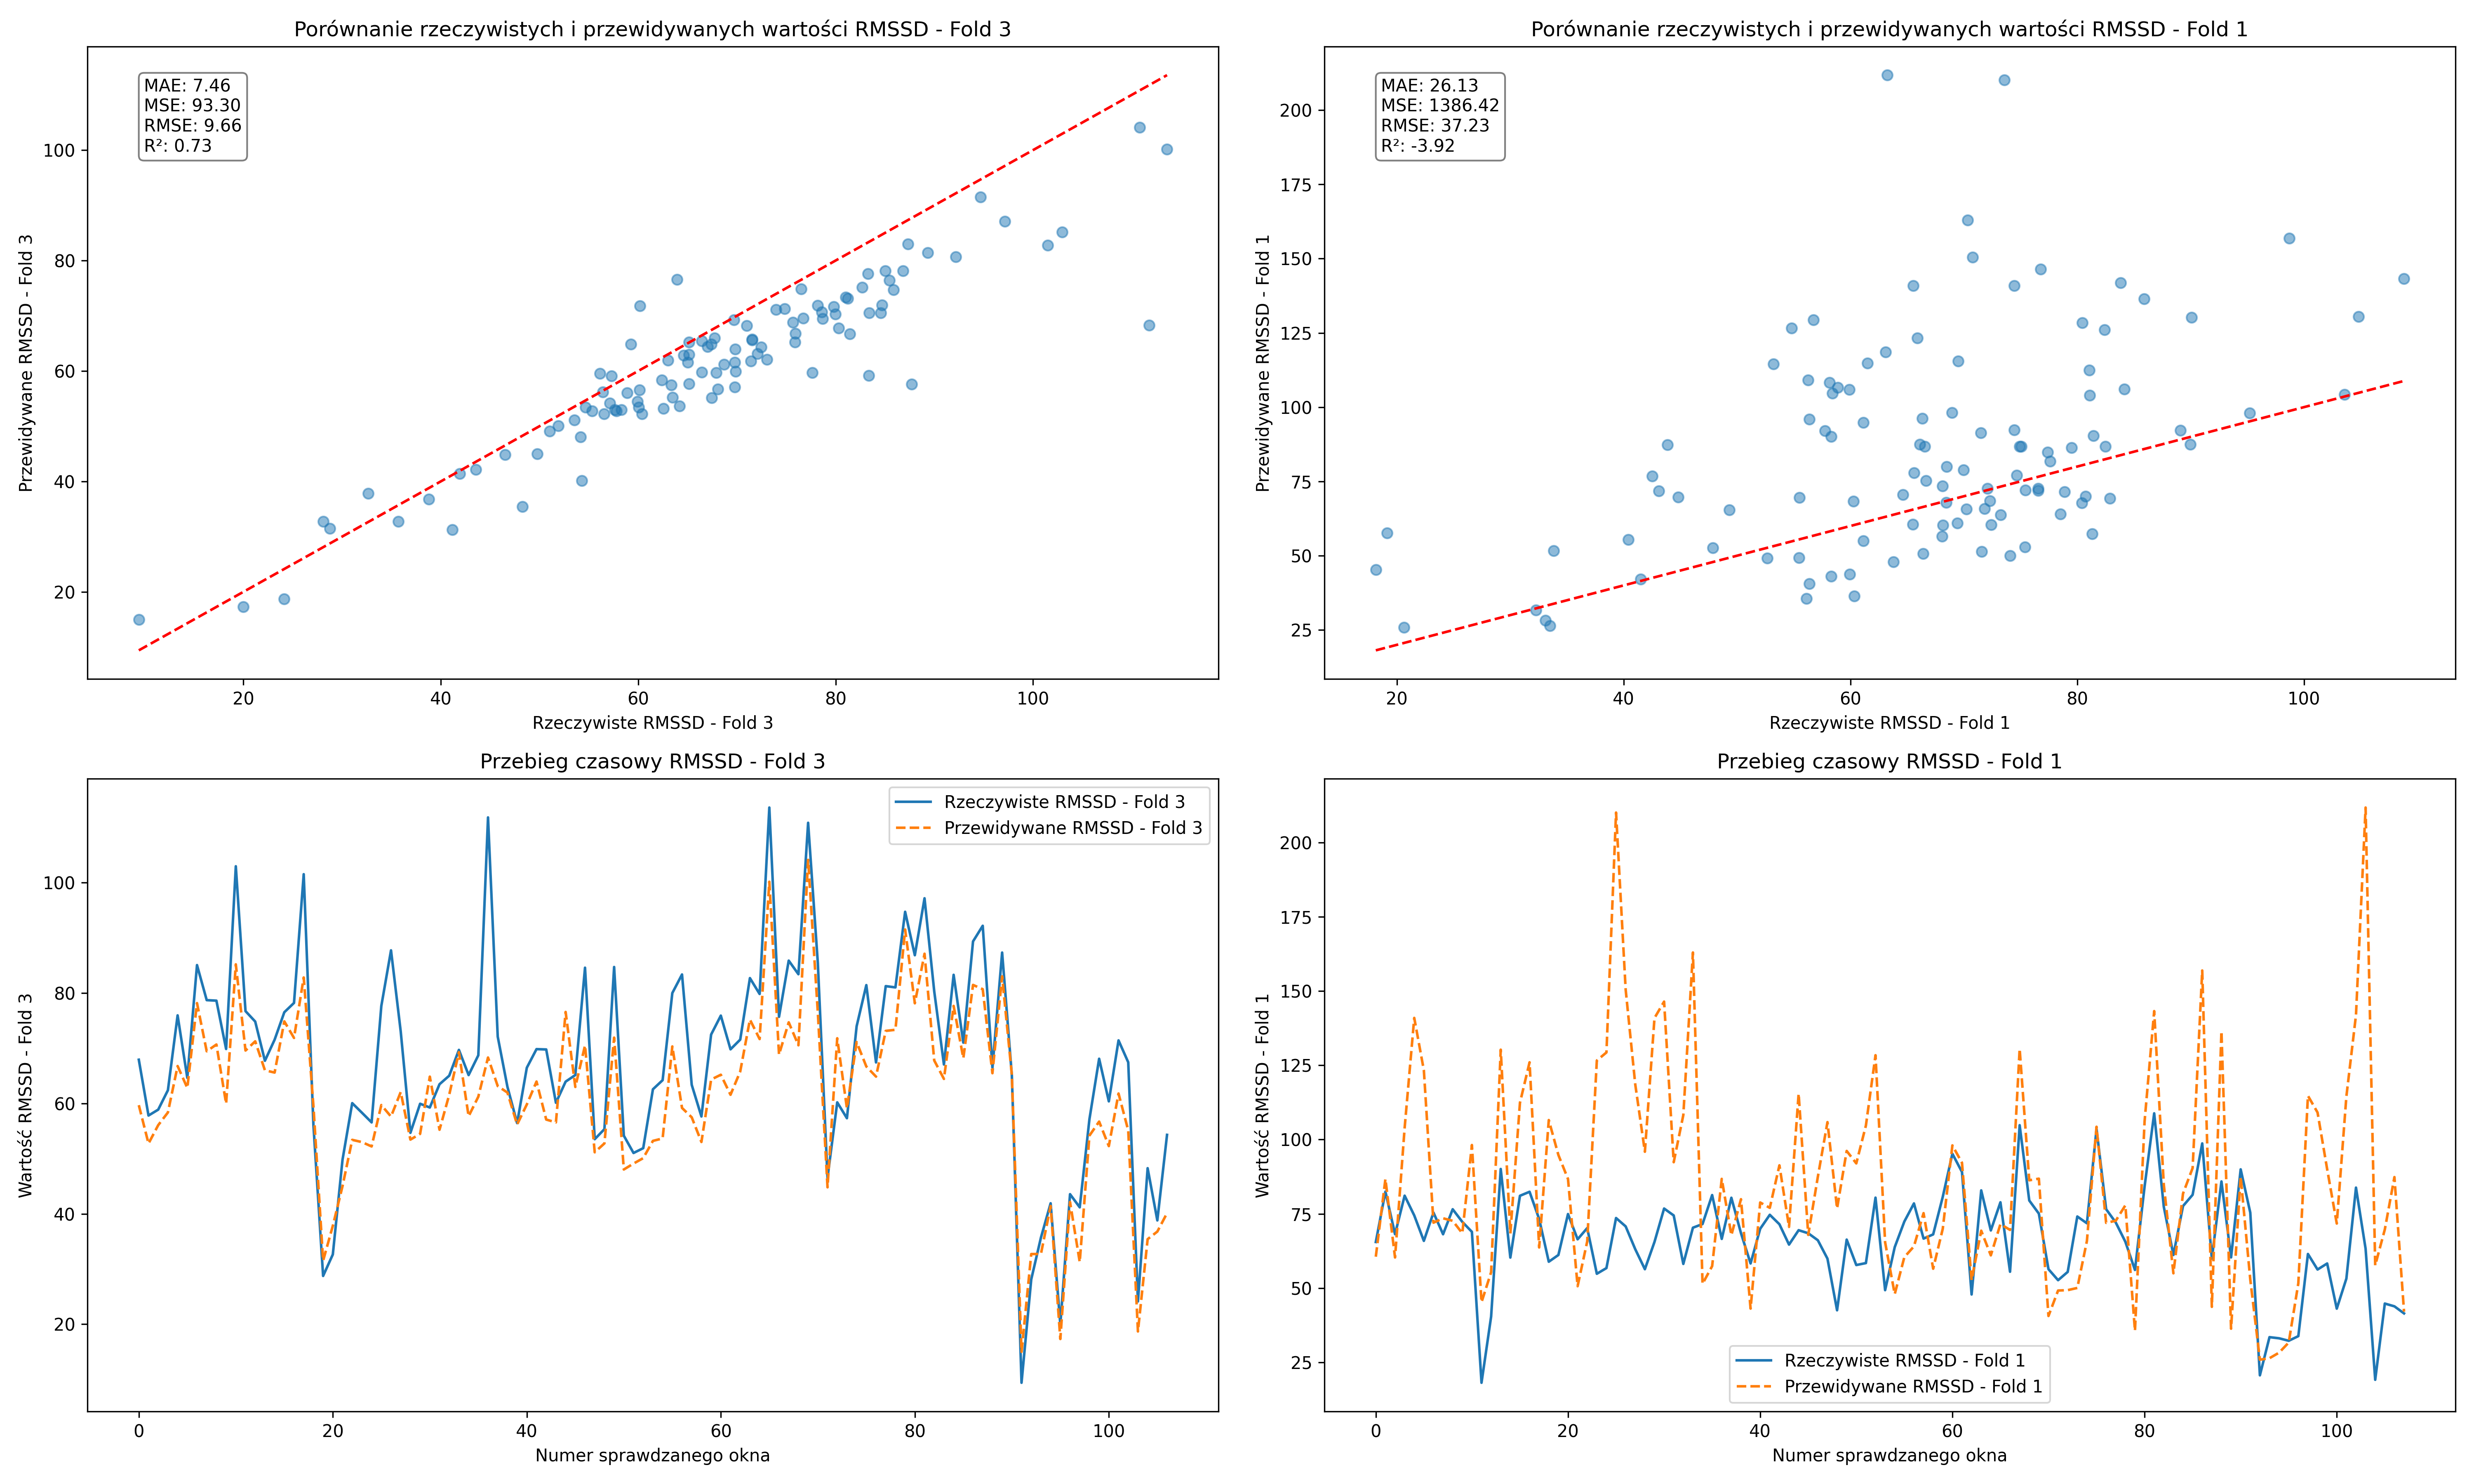
\includegraphics[scale=0.25]{Rysunki/RMSSD_2_folds.png}
    \caption{Wyniki przewidywa� RMSSD dla dw�ch fold�w}
    \label{fig/RMSSD_2_folds}
\end{figure}

\subsection{Wnioski}
Zaproponowany model end-to-end wykaza� si� przyzwoit� dok�adno�cia w wariancie,
w kt�rym przewidywano jednocze�nie warto�ci SDNN oraz RMSSD. Wyniki te nie by�y
jednak na tyle dok�adne, aby uzasadni� u�ycie tego modelu zamiast tradycyjnych
podej��, opartych g��wnie na wcze�niejszym wyznaczeniu za�amk�w R i ich
analizie za pomoc� klasycznych wzor�w. Mimo to warto podkre�li�, �e
zastosowanie modelu end-to-end niesie za sob� istotne zalety, takie jak
prostota u�ycia, ograniczenie liczby etap�w przetwarzania czy kr�tszy czas
analizy. Co wi�cej mo�liwe, �e wytrenowanie tego typu modelu na du�ej ilo�ci,
dobrze oznaczonych danych mog�oby zwi�kszy� jego skuteczno��, umo�liwiaj�c
dok�adne dzia�anie nawet w przypadkach, gdzie wykrywanie za�amk�w R mo�e by�
utrudnione lub niemo�liwe.

Warto przypomnie�, �e przegl�d literatury nie wykaza� wcze�niejszego
zastosowania podej�cia end-to-end do przewidywania metryk HRV oraz RSA
bezpo�rednio z sygna�u EKG. Prezentowane w niniejszej pracy rozwi�zanie ma
zatem charakter nowatorski, a ocena jego skuteczno�ci jest relatywnie trudna ze
wzgl�du na brak wcze�niejszych bada� w tej dziedzinie. Fakt ten w po��czeniu z
dobrze rokuj�cymi wynikami, wskazuje na potencja� rozwojowy tej metody. Dalsze
prace nad jej udoskonaleniem mog� prowadzi� do stworzenia bardziej
uniwersalnego oraz dok�adnego narz�dzia analizy tych metryk.



\chapter{Podsumowanie oraz dyskusja \small{(autor: Jakub Wojtalewicz)}}

Celem niniejszej pracy by�o stworzenie frameworka do odbioru i przetwarzania danych z czujnika Polar H10 oraz opracowanie modelu typu end-to-end, umo�liwiaj�cego wykrywanie okre�lonych wzorc�w w sygnale EKG.
W ramach pracy stworzono aplikacj� po�rednicz�c�, pozwalaj�c� na odbi�r danych z czujnika Polar H10, oraz aplikacj� odpowiedzialn� za analiz� i wy�wietlanie sygna�u EKG oraz jego parametr�w. Do tego zastosowano trzy modele sieci neuronowych, z kt�rych jedna dzia�a�a w modelu end-to-end. W szczeg�lno�ci wykorzystano sie� U-Net, kt�ra w testach wykaza�a si� podobnym poziomem dok�adno�ci na sygnale dobrej jako�ci oraz lepszym w przypadku bardziej realnej sytuacji, tj. sygna�u zaszumionego. Dzi�ki temu posiada wi�kszy potencja� na zastosowanie w praktyce.

Drugi z modeli, maj�cy na celu przewidywanie miar HRV na podstawie interwa��w RR, uzyska� najlepsze rezultaty spo�r�d testowanych metod, jednak w obecnej formie nie znajduje bezpo�redniego zastosowania praktycznego, bior�c pod uwag� fakt, �e dostawa� na wej�cie interwa�y RR, z kt�rych mo�na wyliczy� te miary wprost. Niemniej jednak spos�b dzia�ania tej sieci mo�e okaza� si� kluczowy przy opracowywaniu bardziej zaawansowanego modelu end-to-end.

Najbardziej nowatorskim podej�ciem by�a sie� end-to-end, kt�rej celem by�o bezpo�rednie przewidywanie miar HRV na podstawie surowego sygna�u EKG. Model ten osi�gn�� bardzo dobre wyniki: wsp�czynnik determinacji $R^2$ wynosi� 0,88 dla SDNN oraz 0,58 dla RMSSD. Chocia� trudno por�wna� te wyniki z literatur� naukow� z powodu braku podobnych implementacji, s� one obiecuj�ce i pokazuj� potencja� tego podej�cia w dalszym rozwoju analizy sygna��w EKG.

Warto jednak podkre�li�, �e obecna forma modeli przewiduj�cych miary HRV nie jest jeszcze gotowa do zastosowa� praktycznych. Jedyn� sieci�, kt�ra mo�e znale�� zastosowanie w praktyce ju� teraz, jest U-Net, kt�ry bardzo dobrze radzi sobie z detekcj� za�amk�w R.

Dodatkowo, wszystkie modele by�y testowane g��wnie na danych pochodz�cych od jednego pacjenta oraz z jednego urz�dzenia. Mimo ograniczonego zbioru danych � oko�o 50 godzin nagra� � uda�o si� uzyska� satysfakcjonuj�ce rezultaty. W przysz�ych pracach warto skupi� si� na rozszerzeniu zbioru danych, uwzgl�dniaj�c r�norodnych pacjent�w i urz�dzenia pomiarowe, co pozwoli na zwi�kszenie uniwersalno�ci modeli. Cho� uzyskane wyniki dla SDNN s� zadowalaj�ce, konieczne jest dalsze doskonalenie architektury sieci i jej parametr�w w celu poprawy przewidywania RMSSD. Dodatkowo, integracja analizy sygna�u EKG z innymi biomarkerami, takimi jak sygna�y oddechowe, mog�aby dostarczy� bardziej kompleksowego obrazu stanu zdrowia i otworzy� nowe mo�liwo�ci zastosowa�.

Podsumowuj�c, przeprowadzone badania wykaza�y, �e metody uczenia maszynowego w analizie sygna��w EKG maj� znacz�cy potencja�, cho� wymagaj� dalszego rozwoju. Szczeg�lnie modelowanie typu end-to-end wydaje si� przysz�o�ciowym kierunkiem, kt�ry mo�e znacz�co wp�yn�� na spos�b analizy danych kardiologicznych. Niniejsza praca stanowi solidny punkt wyj�cia dla kolejnych bada�, wskazuj�c zar�wno na zalety, jak i na wyzwania zwi�zane z wykorzystaniem nowoczesnych metod w analizie sygna��w biomedycznych.


\bibliographystyle{plain}
\begin{thebibliography}{99}
    \addcontentsline{toc}{chapter}{Wykaz literatury}
    \small

    %------------------------------------------
    %Lilly, Leonard S. (2016). Pathophysiology of Heart Disease: A Collaborative Project of Medical Students and Faculty, 6th Edition. Lippincott Williams & Wilkins. pp. 70�78. ISBN 978-1-4698-9758-5. OCLC 1229852550.

    \bibitem{Lilly-Pathophysiology}
    Leonard S. Lilly \emph{Pathophysiology of Heart Disease: A Collaborative Project of Medical Students and Faculty, 6th Edition.} Lippincott Williams \& Wilkins. pp. 70�78. ISBN 978-1-4698-9758-5. OCLC 1229852550.
    %------------------------------------------

    %------------------------------------------
    \bibitem{Malik-HRV}
    Task Force of the European Society of Cardiology, \& North American Society of Pacing and Electrophysiology \emph{Heart rate variability: Standards of measurement, physiological interpretation, and clinical use.} In: Circulation. 1996, pp. 1043-1065. doi:10.1161/01.CIR.93.5.1043.
    %PDF
    %https://www.ahajournals.org/doi/10.1161/01.CIR.93.5.1043
    %https://www.researchgate.net/publication/279548912_Heart_rate_variability_Standards_of_measurement_physiological_interpretation_and_clinical_use
    %------------------------------------------

    %------------------------------------------
    \bibitem{Fariha-PanTompkins}
    M. A. Z. Fariha et al. \emph{Analysis of Pan-Tompkins Algorithm Performance with Noisy ECG Signals}, J. Phys.: Conf. Ser., vol. 1532, p. 012022, 2020. Available at: \href{https://iopscience.iop.org/article/10.1088/1742-6596/1532/1/012022/pdf}{https://iopscience.iop.org/article/10.1088/1742-6596/1532/1/012022/pdf.} [Accessed 08.11.2024]
    %https://iopscience.iop.org/article/10.1088/1742-6596/1532/1/012022/pdf}{https://iopscience.iop.org/article/10.1088/1742-6596/1532/1/012022/pdf
    %------------------------------------------

    %TO DO: dopasowa� strony glownie rozdzial 2
    \bibitem{Romano-ECG}
    M. Roman{\`o} and R. Bertona. \emph{Text Atlas of Practical Electrocardiography: A Basic Guide to ECG Interpretation.} Springer Milan, 2015. ISBN: 9788847057418. %Available at: \href{https://books.google.pl/books?id=qH8QBwAAQBAJ}{https://books.google.pl/books?id=qH8QBwAAQBAJ}. [Accessed 12.11.2024]

    % https://books.google.pl/books?hl=pl&lr=&id=qH8QBwAAQBAJ&oi=fnd&pg=PP17&dq=The+Practical+Guide+to+ECG+Interpretation&ots=xtUWsyms0z&sig=GFw3_NCeNPsIWaDzl1LhZNcJ4pY&redir_esc=y#v=onepage&q=The%20Practical%20Guide%20to%20ECG%20Interpretation&f=false
    %https://books.google.pl/books?id=qH8QBwAAQBAJ&printsec=frontcover&hl=pl&source=gbs_atb#v=onepage&q&f=false

    \bibitem{Goodfellow-DeepLearning}
    I. Goodfellow, Y. Bengio, and A. Courville, \emph{Deep Learning}. Cambridge, MA, USA: MIT Press, 2016. [Online]. Available: \url{http://www.deeplearningbook.org}[Accessed 25.11.2024]

    %------------------------------------------
    \bibitem{Bartsch-PhaseTransitions}
    R. P. Bartsch, A. Y. Schumann, J. W. Kantelhardt, T. Penzel, and P. Ch. Ivanov,
    \emph{Phase transitions in physiologic coupling},
    Proc. Natl. Acad. Sci. U. S. A., vol. 109, no. 26, pp. 10181�10186, Jun. 2012.
    Available at: \href{https://doi.org/10.1073/pnas.1204568109}{https://doi.org/10.1073/pnas.1204568109}. [Accessed 08.11.2024]
    %------------------------------------------

    \bibitem{MUzairZahid-UNET}
    M. U. Zahid, S. Kiranyaz, T. Ince, O. C. Devecioglu, M. E. H. Chowdhury, A. Khandakar, A. Tahir, and M. Gabbouj,
    \emph{Robust R-Peak Detection in Low-Quality Holter ECGs Using 1D Convolutional Neural Network},
    *IEEE Transactions on Biomedical Engineering*, vol. 69, no. 1, pp. 119--128, Jan. 2021.

    \bibitem{FDA_KardiaAI_2018}
    U.S. Food and Drug Administration, \emph{Kardia AI Clearance - K181823}, 2018. [Online]. Available: \url{https://www.accessdata.fda.gov/cdrh_docs/pdf18/K181823.pdf}. [Accessed: Dec. 1, 2024].

    % Bumgarner, J. M., Lambert, C. T., Hussein, A. A., et al. (2018). Smartwatch Algorithm for Automated Detection of Atrial Fibrillation. Journal of the American College of Cardiology, 71(21), 2381-2388. DOI: 10.1016/j.jacc.2018.03.003.
    \bibitem{Bumgarner2018}
    J.~M. Bumgarner, C.~T. Lambert, A.~A. Hussein, \textit{et al.}, ``Smartwatch Algorithm for Automated Detection of Atrial Fibrillation,'' \textit{Journal of the American College of Cardiology}, vol. 71, no. 21, pp. 2381--2388, 2018, doi: \url{10.1016/j.jacc.2018.03.003}.

    % https://pmc.ncbi.nlm.nih.gov/articles/PMC9971999/
    \bibitem{Raghunath2023}
    A. Raghunath, D.~D. Nguyen, M. Schram, D. Albert, S. Gollakota, L. Shapiro, and A.~R. Sridhar, ``Artificial intelligence-enabled mobile electrocardiograms for event prediction in paroxysmal atrial fibrillation,'' \textit{Cardiovascular Digital Health Journal}, vol. 4, no. 1, pp. 21--28, Jan. 2023, doi: \url{10.1016/j.cvdhj.2023.01.002}. PMID: 36865584; PMCID: PMC9971999.

    \bibitem{ribeiro2020automatic}
    Ribeiro, A.H., Ribeiro, M.H., Paix?o, G.M.M. \emph{et al.}, \emph{Automatic diagnosis of the 12-lead ECG using a deep neural network}, \emph{Nature Communications}, vol. 11, p. 1760, 2020, doi: 10.1038/s41467-020-15432-4.
    % Ribeiro, A.H., Ribeiro, M.H., Paix?o, G.M.M. et al. Automatic diagnosis of the 12-lead ECG using a deep neural network. Nat Commun 11, 1760 (2020). https://doi.org/10.1038/s41467-020-15432-4

    \bibitem{NAROTAMO-deepLearning}
    Deep learning for ECG classification: A comparative study of 1D and 2D representations and multimodal fusion approaches
    %     @article{NAROTAMO2024106141,
    % title = {Deep learning for ECG classification: A comparative study of 1D and 2D representations and multimodal fusion approaches},
    % journal = {Biomedical Signal Processing and Control},
    % volume = {93},
    % pages = {106141},
    % year = {2024},
    % issn = {1746-8094},
    % doi = {https://doi.org/10.1016/j.bspc.2024.106141},
    % url = {https://www.sciencedirect.com/science/article/pii/S174680942400199X},
    % author = {Hemaxi Narotamo and Mariana Dias and Ricardo Santos and Andr� V. Carreiro and Hugo Gamboa and Margarida Silveira},
    % keywords = {Electrocardiogram classification, Cardiovascular diseases, Deep learning, Recurrent neural networks, Convolutional neural networks, Multimodal artificial intelligence},
    % abstract = {The improved diagnosis of cardiovascular diseases (CVD) from electrocardiograms (ECG) may help prevent their severity. Since Deep Learning (DL) became popular, several DL methods have been developed for ECG classification. In this work, we compare how different methods for ECG signal representation perform in the multi-label classification of CVDs, including recent attention-based strategies. Furthermore, multimodal fusion strategies are employed to improve the prediction capacity of individual representation networks. The publicly available PTB-XL ECG dataset, which contains 21,837 records and labels for the diagnosis of 4 CVDs, was used for the task. Two DL strategies using different processing approaches were compared. Recurrent Neural Network-based models take advantage of the temporal dependence between raw signal values, namely through Gated Recurrent Unit (GRU), Long Short Term Memory (LSTM) and 1D-Convolutional Neural Network models. Additionally, the raw ECG was converted into image representations, based on recent work, and the classification was performed using distinct 2D-Convolutional Neural Networks. The potential of multimodal DL was then studied through early, late and joint data fusion strategies, to evaluate the benefit of resorting to multiple representations. Results based on the 1D ECG representation outperform image-based approaches and multimodal models. The best model, GRU, achieved sensitivity and specificity of 79.67% and 81.04%, respectively.}
    % }

    \bibitem{Morteza-RandomForest}
    Morteza Zabihi1*
    , Ali Bahrami Rad2*
    , Aggelos K. Katsaggelos3
    ,
    Serkan Kiranyaz4
    , Susanna Narkilahti2
    , and Moncef Gabbouj Detection of Atrial Fibrillation in ECG Hand-held Devices Using a Random
    Forest Classifier
    % https://physionet.org/files/challenge-2017/1.0.0/papers/069-336.pdf

    \bibitem{Bachmann-electrolyte_prediction}
    von Bachmann, P., Gedon, D., Gustafsson, F.K. et al. \emph{Evaluating regression and probabilistic methods for ECG-based electrolyte prediction.} Sci Rep 14, 15273 (2024). https://doi.org/10.1038/s41598-024-65223-w
    % von Bachmann, P., Gedon, D., Gustafsson, F.K. et al. Evaluating regression and probabilistic methods for ECG-based electrolyte prediction. Sci Rep 14, 15273 (2024). https://doi.org/10.1038/s41598-024-65223-w

    \bibitem{JUHO-LSTM}
    Laitala J., Jiang M., Haulivuori E., Kasaeyan Naeini E., Airola A., Rahmani A. M., Dutt N., Liljeberg P.:
    Robust ECG R-peak detection using LSTM, 2020, doi: 10.1145/3341105.3373945.
    %https://dl.acm.org/doi/pdf/10.1145/3341105.3373945

    \bibitem{PhysioNet-Challange2017}
    Clifford GD, Liu C, Moody B, Li-wei HL, Silva I, Li Q, Johnson AE, Mark RG. AF classification from a short single lead ECG recording: The PhysioNet/computing in cardiology challenge 2017. In 2017 Computing in Cardiology (CinC) 2017 Sep 24 (pp. 1-4). IEEE. https://doi.org/10.22489/CinC.2017.065-469

    \bibitem{Kavya-shockableArthytmiaDetection}
    Lakkakula Kavya, Karuna Yepuganti, Saladi Saritha, Allam Jaya Prakash, Kiran Kumar Patro, Suraj Prakash Sahoo, Ryszard Tadeusiewicz, Pawel Plawiak:
    A review of shockable arrhythmia detection of ECG signals using machine and deep learning techniques. Int. J. Appl. Math. Comput. Sci. 34
    % https://sciendo.com/article/10.61822/amcs-2024-0034


    \bibitem{Irungu-EcgCovid}
    J. Irungu, T. Oladunni, A. C. Grizzle, M. Denis, M. Savadkoohi, and E. Ososanya, "ML-ECG-COVID: A Machine Learning-Electrocardiogram Signal Processing Technique for COVID-19 Predictive Modeling," \textit{IEEE Access}, vol. 11, pp. 135994--136014, 2023, doi: 10.1109/ACCESS.2023.3335384.


%     @ARTICLE{10325461,
%   author={Irungu, John and Oladunni, Timothy and Grizzle, Andrew C. and Denis, Max and Savadkoohi, Marzieh and Ososanya, Esther},
%   journal={IEEE Access}, 
%   title={ML-ECG-COVID: A Machine Learning-Electrocardiogram Signal Processing Technique for COVID-19 Predictive Modeling}, 
%   year={2023},
%   volume={11},
%   number={},
%   pages={135994-136014},
%   keywords={Electrocardiography;Feature extraction;Support vector machines;Machine learning;Classification algorithms;Time-frequency analysis;Random forests;Nearest neighbor methods;Support vector machine (SVM);random forest;QRS complex;K-nearest neighbor (KNN);electrocardiogram (ECG)},
%   doi={10.1109/ACCESS.2023.3335384}}




    \bibitem{SAKR2023324}
    A.~S.~Sakr, P.~P�awiak, R.~Tadeusiewicz, J.~P�awiak, M.~Sakr, and M.~Hammad, "ECG-COVID: An end-to-end deep model based on electrocardiogram for COVID-19 detection," *Information Sciences*, vol. 619, pp. 324�339, 2023, doi: https://doi.org/10.1016/j.ins.2022.11.069

    %     @article{SAKR2023324,
    % title = {ECG-COVID: An end-to-end deep model based on electrocardiogram for COVID-19 detection},
    % journal = {Information Sciences},
    % volume = {619},
    % pages = {324-339},
    % year = {2023},
    % issn = {0020-0255},
    % doi = {https://doi.org/10.1016/j.ins.2022.11.069},
    % url = {https://www.sciencedirect.com/science/article/pii/S0020025522013585},
    % author = {Ahmed S. Sakr and Pawe� P�awiak and Ryszard Tadeusiewicz and Joanna P�awiak and Mohamed Sakr and Mohamed Hammad},
    % keywords = {COVID-19, ECG, CNN, End-to-end, Deep learning}

    \bibitem{Coutts-HRV}
    L. V. Coutts, D. Plans, A. W. Brown, and J. Collomosse, "Deep learning with wearable based heart rate variability for prediction of mental and general health," Journal of Biomedical Informatics, vol. 112, p. 103610, 2020. doi: 10.1016/j.jbi.2020.103610.

    % @article{COUTTS2020103610,
    % title = {Deep learning with wearable based heart rate variability for prediction of mental and general health},
    % journal = {Journal of Biomedical Informatics},
    % volume = {112},
    % pages = {103610},
    % year = {2020},
    % issn = {1532-0464},
    % doi = {https://doi.org/10.1016/j.jbi.2020.103610},
    % url = {https://www.sciencedirect.com/science/article/pii/S1532046420302380},
    % author = {Louise V. Coutts and David Plans and Alan W. Brown and John Collomosse},
    % keywords = {Machine learning, LSTM, Heart rate variability, Mental health, Wearables},
    % abstract = {The ubiquity and commoditisation of wearable biosensors (fitness bands) has led to a deluge of personal healthcare data, but with limited analytics typically fed back to the user. The feasibility of feeding back more complex, seemingly unrelated measures to users was investigated, by assessing whether increased levels of stress, anxiety and depression (factors known to affect cardiac function) and general health measures could be accurately predicted using heart rate variability (HRV) data from wrist wearables alone. Levels of stress, anxiety, depression and general health were evaluated from subjective questionnaires completed on a weekly or twice-weekly basis by 652 participants. These scores were then converted into binary levels (either above or below a set threshold) for each health measure and used as tags to train Deep Neural Networks (LSTMs) to classify each health measure using HRV data alone. Three data input types were investigated: time domain, frequency domain and typical HRV measures. For mental health measures, classification accuracies of up to 83% and 73% were achieved, with five and two minute HRV data streams respectively, showing improved predictive capability and potential future wearable use for tracking stress and well-being.}
    % }


    \bibitem{andrea-termo}
    Estimation of Heart Rate Variability Parameters by Machine Learning Approaches Applied to Facial Infrared Thermal Imaging
    %https://www.frontiersin.org/journals/cardiovascular-medicine/articles/10.3389/fcvm.2022.893374/full


    \bibitem{Gudny-ppgHRV}
    Gudny Bjork Odinsdottir, Jesper Larsson Deep Learning Approach for Extracting Heart Rate Variability from a Photoplethysmographic Signal

   
    \bibitem{Morales-RSASVM}
    Morales J, Borz�e P, Testelmans D, Buyse B, Van Huffel S, Varon C. Linear and Non-linear Quantification of the Respiratory Sinus Arrhythmia Using Support Vector Machines. Front Physiol. 2021 Feb 5;12:623781. doi: 10.3389/fphys.2021.623781. PMID: 33633586; PMCID: PMC7901929.
    % https://pmc.ncbi.nlm.nih.gov/articles/PMC7901929/

    \bibitem{Lahr-RSA}
    Peyton Lahr 1,2,Chloe Carling 1,Joseph Nauer 1,Ryan McGrath 1,* andJames W. Grier
    James W. Grier,  Supervised Machine Learning to Examine Factors Associated with Respiratory Sinus Arrhythmias and Ectopic Heart Beats in Adults: A Pilot Study
 
% https://www.mdpi.com/2673-3846/5/3/20

% https://iris.unipa.it/retrieve/handle/10447/483248/1119979/112-Morales-IEEE_TBME_2020-preprint.pdf

\end{thebibliography}

\renewcommand{\baselinestretch}{1.0}\normalsize	
\addcontentsline{toc}{chapter}{\listfigurename}
\listoffigures			

\chapter*{Dodatek A}
\addcontentsline{toc}{chapter}{Dodatek A}
\noindent Kod �rod�owy wytworzony w trakcie tworzenia pracy dyplomowej dost�pny jest pod adresem: \href{https://github.com/PiotrexOG/ECG}{https://github.com/PiotrexOG/ECG}

\end{document}